\documentclass[11pt]{article}

\usepackage{apacite}
\usepackage{amsmath,amssymb}
\usepackage{graphicx}
\usepackage{color}
\usepackage{url}
\usepackage{fullpage}
\usepackage{setspace}
\usepackage{booktabs}
\usepackage{multirow}
\usepackage{lingmacros}
\usepackage{caption}
\usepackage{subcaption}
\usepackage{tablefootnote}
\usepackage{fancyvrb}

%\newcommand{\url}[1]{$#1$}

\definecolor{Blue}{RGB}{50,50,200}
\newcommand{\blue}[1]{\textcolor{Blue}{#1}}

\definecolor{Red}{RGB}{255,0,0}
\newcommand{\red}[1]{\textcolor{Red}{#1}}
\newcommand{\jd}[1]{\textcolor{Red}{[jd: #1]}} 

\definecolor{Green}{RGB}{50,200,50}
\newcommand{\ndg}[1]{\textcolor{Green}{[ndg: #1]}}  

\definecolor{Purple}{RGB}{128,0,128}
\newcommand{\cg}[1]{\textcolor{Purple}{[cg: #1]}} 

\newcommand{\denote}[1]{\mbox{ $[\![ #1 ]\!]$}}

\newcommand{\subsubsubsection}[1]{{\em #1}}
\newcommand{\eref}[1]{(\ref{#1})}
\newcommand{\tableref}[1]{Table \ref{#1}}
\newcommand{\figref}[1]{Figure \ref{#1}}
\newcommand{\appref}[1]{Appendix \ref{#1}}
\newcommand{\sectionref}[1]{Section \ref{#1}}

\VerbatimFootnotes

\title{Over overinformativeness: rationally redundant referring expressions}

 
\author{{\large \bf Judith Degen, Caroline Graf, Robert X.D.~Hawkins, Elisa Kreiss, \& Noah D.~Goodman} \\
  \{jdegen\}@stanford.edu\\
  Department of Psychology, 450 Serra Mall \\
  Stanford, CA 94305 USA}

\begin{document}

\maketitle


\begin{abstract}
Referring is one of the most basic and prevalent uses of language. How do speakers choose from the wealth of referring expressions at their disposal? Rational theories of language use have come under attack for decades for not being able to account for the seemingly irrational overinformativeness ubiquitous in referring expressions. Here we present a novel production model of referring expressions within the Rational Speech Act framework that treats speakers as agents that rationally trade off cost and informativeness of utterances. Crucially, the assumption of deterministic meanings is relaxed. This allows us to capture a large number of seemingly disparate phenomena within one unified framework: the basic asymmetry in speakers' propensity to overmodify with color rather than size; the increase in overmodification in complex scenes; the increase in overmodification with atypical features; and the preference for basic level reference in nominal reference. The findings cast a new light on the production of referring expressions: rather than being wastefully overinformative, reference is rationally redundant. This implicates a production system geared towards communicative efficiency.

\textbf{Keywords:} 
reference; referring expressions; informativeness; probabilistic pragmatics; experimental pragmatics
\end{abstract}

\tableofcontents

\section{Introduction}
\label{sec:intro}

Reference to objects is one of the most basic and prevalent uses of language. This requires speakers to choose from amongst a wealth of referring expressions they have at their disposal. How does a speaker choose whether to refer to an object as \emph{the animal}, \emph{the dog}, \emph{the dalmatian}, or \emph{the big mostly white dalmatian}? The context within which the object occurs (other non-dogs, other dogs, other dalmatians) plays a large part in determining which features the speaker chooses to include in their utterance -- speakers aim to be sufficiently informative to uniquely establish reference to the intended object. However, speakers' utterances often exhibit what has been claimed to be \emph{overinformativeness}: referring expressions are often more specific than necessary for establishing unique reference, and they are so in systematic ways. Providing a unified theory for speakers' systematic patterns of overinformativeness has so far proved elusive.

This paper is concerned with accounting for these systematic patterns in overinformative referring expressions (REs). We restrict ourselves to definite descriptions of the form \emph{the (ADJ}?\emph{)}+ \emph{NOUN}, that is, noun phrases that minimally contain the definite determiner \emph{the} followed by a head noun, with any number of adjectives occurring between the determiner and the noun.\footnote{In contrast, we will \emph{not} provide a treatment of pronominal referring expressions, indefinite descriptions, names, or definite descriptions with post-nominal modification, though we offer some speculative remarks on how the approach outlined here can be applied to these cases. \jd{make sure to pick this back up in the discussion}} A model of these REs will allow us to unify two domains in language production that have been typically treated as separate, and that have typically been treated as interesting for different reasons: the production of so-called overmodified referring expressions on the one hand, which a lot of literature in language production has been devoted to \cite{herrmann1976, Pechmann1989, nadig2002, Maes2004, Engelhardt2006, Arts2011, Koolen2011, rubiofernandez2016}; and the production of simple nominal expressions, which has so far mostly received attention in the concepts and categorization literature \cite{Rosch1973, Rosch1976} \cg{@jd: "Adele Goldberg?" Do you mean to cite her book "Constructions at Work. The Nature of Generalization"? If yes, you can use the citation key goldberg2006constructions. Among others, Beach (1964), Reed (1972), Murphy \& Smith (1982), and Cruse (1977) also did work on this, perhaps we want to cite them also? reed1972pattern, beach1964cue, murphy1982basic, cruse1977pragmatics}. In the following, we review some of the key phenomena and puzzles in each of these literatures. We then present a model of RE production within the Rational Speech Act framework \cite{frank2012, goodman2016}, which treats speakers as boundedly rational agents who optimize the tradeoff between utterance cost and informativeness. Our key innovation is to relax the assumption that semantic truth functions are deterministic. Treating speakers as boundedly rational agents operating on a continuous semantics captures that adding seemingly overinformative modifiers or using seemingly too specific nouns can be useful and informative, to the extent that not doing so would be too likely to lead a listener to incorrectly infer the speaker's intention (or to invest too much processing effort in inferring the speaker's correct intention) \jd{make this cleaner?}. We thus for the first time provide a unified explanation for a number of seemingly disparate phenomena from the modified and nominal RE literature. 

We spend the remainder of the paper demonstrating how the account applies to various phenomena. In \sectionref{sec:intro} we spell out the problem and introduce the overinformativeness phenomena to capture. In \sectionref{sec:models} we introduce the basic (deterministic semantics) and modified (continuous semantics) Rational Speech Act framework. In Sections 3 - 5 we evaluate the continuous semantics RSA model on data from interactive online reference game experiments that exhibit the phenomena introduced in \sectionref{sec:intro}: size and color modifier choice under varying conditions of scene complexity; typicality effects in the choice of color modifier; and choice of nominal level of reference. We wrap up in \sectionref{sec:gd} by summarizing our findings and discussing the far-reaching implications of and further challenges for this line of work.

\subsection{Production of referring expressions: a case against rational language use?}

How should a cooperative choose between competing referring expressions? Grice, in his seminal work, provided some guidance by formulating his famous conversational maxims, intended as a guide to listeners' expectations about good speaker behavior \cite{grice1975}. His maxim of Quantity, consisting of two parts, requires of speakers to:

\begin{enumerate}
	\item \emph{Quantity-1:} Make your contribution as informative as is required (for the purposes of the exchange).
	\item \emph{Quantity-2:} Do not make your contribution more informative than is required.
\end{enumerate}

That is, speakers should aim to produce neither under- nor overinformative utterances. While much support has been found for the former \cite{brennan1996, brown1958words, olson1970language, levinson1983pragmatics}, speakers seem remarkably happy to systematically violate Quantity-2. In modified referring expressions, they routinely produce modifiers that are not necessary for uniquely establishing reference (e.g., \emph{the small blue pin} instead of \emph{the small pin} in contexts like \figref{fig:sizesufficient} \cite{gatt2011, Gatt2014, Arts2011, Koolen2011}). In simple nominal expressions, speakers routinely choose to refer to an object with a basic level term even when a superordinate level term would have been sufficient for establishing reference (e.g., \emph{the dog} instead of \emph{the animal} in contexts like \figref{fig:dogcontexts} \cite{Rosch1976, hoffmann1983objektidentifikation, TanakaTaylor91_BasicLevelAndExpertise, Johnson1997, brown1958words}).

These observations have posed a challenge for theories of language production, especially those positing rational language use (including the Gricean one): why this extra expenditure of useless effort? Why this seeming blindness to the level of informativeness requirement? Many have argued from these observations that speakers are in fact not economical \cite{Engelhardt2006, Pechmann1989}. Some have derived a built-in preference for referring at the basic level from considerations of perceptual factors such as shape \cite{Rosch1976, Rosch1973, murphy1982basic}. Others have argued for salience-driven effects on willingness to overmodify \cite{Gatt2014, Westerbeek2015}. In all cases, it is argued that informativeness cannot be the key factor in determining the content of speakers' referring expressions. 

Here we revisit this claim and show that systematically relaxing the requirement of a deterministic semantics for referring expressions also systematically changes the informativeness of utterances. This results in a reconceptualization of what have been termed \emph{overinformative referring expressions} as \emph{rationally redundant referring expressions}. We begin by reviewing the phenomena of interest that a revised theory of definite referring expressions should be able to account for. 

\subsection{Modified referring expressions}
\label{sec:modified}


Most of the literature on overinformative referring expressions has been devoted to the use of overinformative modifiers in modified referring expressions. The prevalent observation is that speakers frequently do not include only the minimal modifiers required for establishing reference, but often also include redundant modifiers \cite{Pechmann1989, nadig2002, Maes2004, Engelhardt2006, Arts2011, Koolen2011}. However, not all modifiers are created equal: there are systematic differences in the overmodification patterns observed for size adjectives (e.g., \emph{big, small}), color adjectives (e.g., \emph{blue, red}), material adjectives (e.g., \emph{plastic, wooden}), and others \cite{sedivy2003a}. Here we review some key patterns of overmodification that have plagued that literature, before spelling out our account of these phenomena in \sectionref{sec:models}.



\begin{figure}
\begin{subfigure}{.5\textwidth}
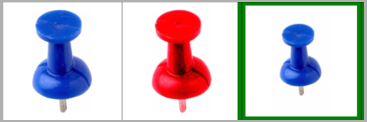
\includegraphics[width=\textwidth]{pics/size-sufficient.png}
\caption{Size sufficient.}
\label{fig:sizesufficient}
\end{subfigure}
\begin{subfigure}{.5\textwidth}
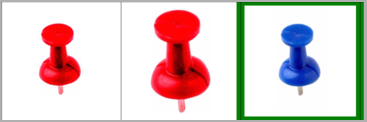
\includegraphics[width=\textwidth]{pics/color-sufficient.png}
\caption{Color sufficient.}
\label{fig:colorsufficient}
\end{subfigure}
\caption{Example contexts where (a) size only or (b) color only is sufficient for unique reference. A green border marks the intended referent.}
\label{fig:pin}
\end{figure}

\begin{figure}
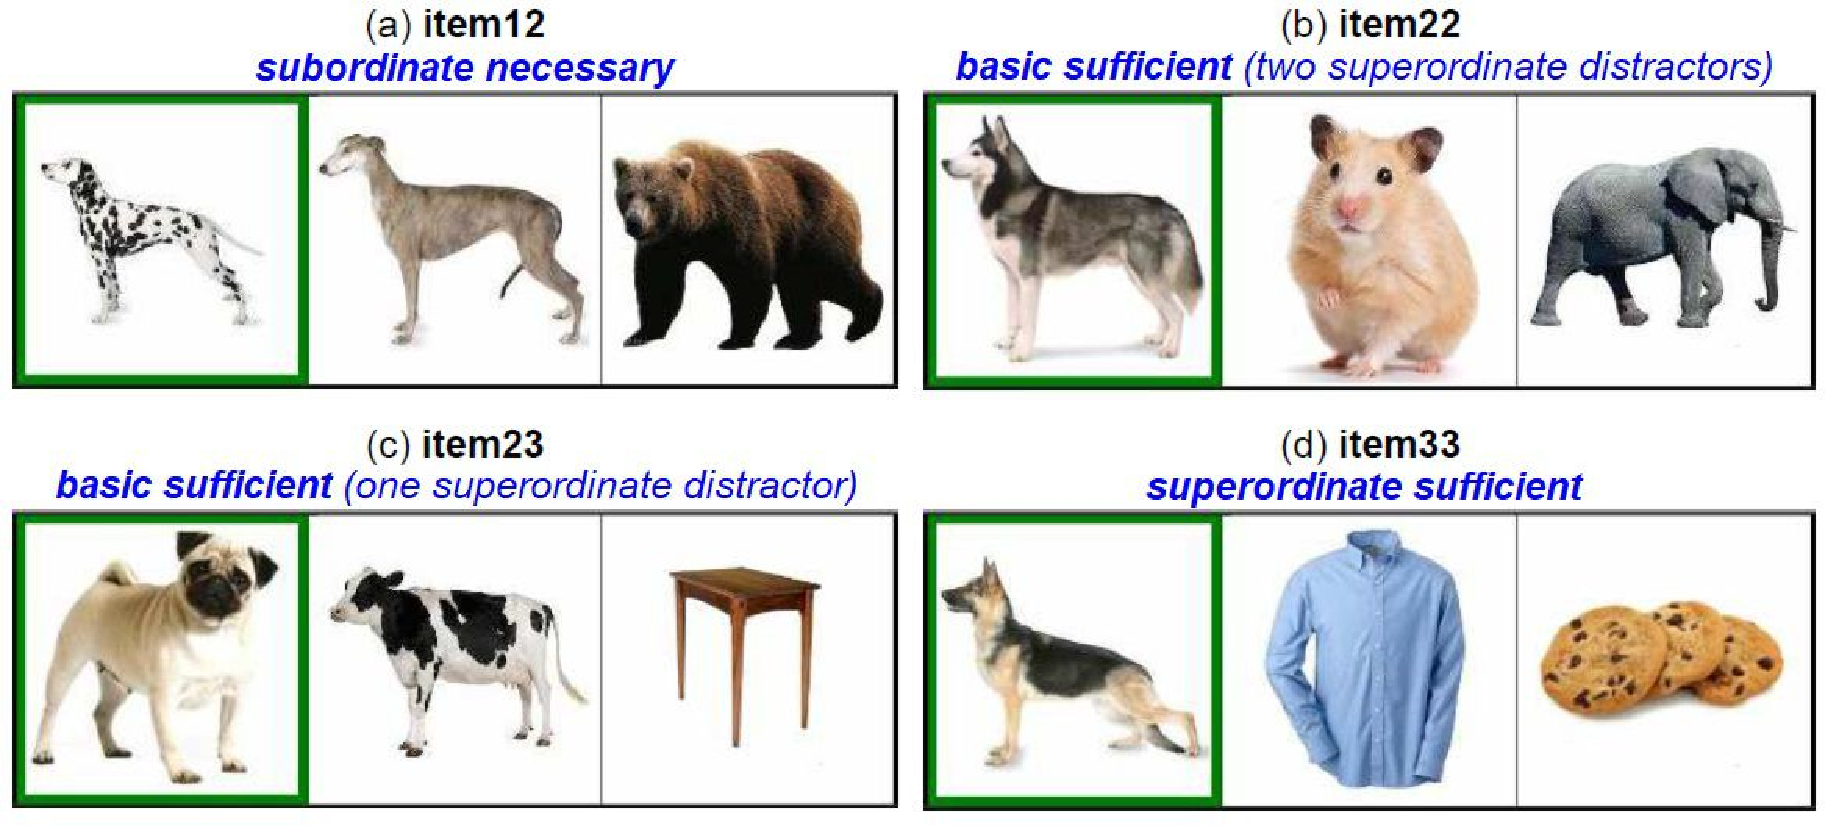
\includegraphics[width=\textwidth]{pics/design}
\caption{Example contexts in which different levels of reference are necessary for establishing unique reference to the target marked with a green border: (a) sub (\emph{dalmatian}), (b, c) basic (\emph{dog}), or (d) super (\emph{animal}).}
\label{fig:dogcontexts}
\end{figure}

\subsubsection{Asymmetry in redundant use of color and size adjectives}
\label{sec:asymmetry}

 In \figref{fig:sizesufficient}, singling out the object highlighted by the green border requires only mentioning its size (\emph{the small pin}). But it is now well-documented that speakers routinely include redundant color adjectives (\emph{the small blue pin}) which are not necessary for uniquely singling out the intended referent in these kinds of contexts \cite{Pechmann1989, Belke2002, gatt2011}. However, the same is not true for size: in contexts like \figref{fig:colorsufficient}, where color is sufficient for unique reference (\emph{the blue pin}), speakers overmodify much more rarely. \tableref{tab:colorsizeasymmetry} shows proportions of color, size, and (overinformative) color-and-size mentions in conditions like those depicted in \figref{fig:pin} across different experiments. In all cases there is a preference for overmodifying with color but not with size.\footnote{There is quite a bit of variation in the actual numbers. We will discuss this variation in the Discussion of \sectionref{sec:rsaevaluationbasicscene}.\jd{correct section ref? do we even discuss this?}}
 
 \begin{table}
 \caption{Proportions of minimally informative \emph{color} (only) or \emph{size} (only) and overinformative \emph{color\_size} mentions in color-sufficient vs.~size-sufficient conditions across experiments.\jd{keep filling in. this is just here for us -- can throw out for the purpose of paper submission}}
 	\begin{tabular}{l l l l l l l l}
	\toprule
	 & & \multicolumn{3}{c}{Color sufficient} & \multicolumn{3}{c}{Size sufficient} \\
	Study & Language & \emph{color} & \emph{size} & \emph{color\_size} & \emph{color} & \emph{size} & \emph{color\_size} \\
	\midrule
	\citeA{Pechmann1989} & Dutch & 99 & 0 & 1 & 9 & 36 & 55 \\
	\citeA{gatt2011} & English & 92 & 0 & 8 & 3 & 17 & 80\\
 	\citeA{gatt2011} & Dutch & 90 & 0 & 10 & 0 & 21 & 79 \\	
 Our baseline study & English & 94 & 0 & 6 & 2 & 52 & 46 \\ 
	\bottomrule
	\end{tabular}
	\label{tab:colorsizeasymmetry}
 \end{table}

Explanations for this asymmetry have varied. \citeA{Pechmann1989} was the first to take the asymmetry as evidence for speakers following an incremental strategy of object naming: speakers initially start to articulate an adjective denoting a feature that listeners can quickly and easily recognize (i.e., color) before they have fully inspected the display and extracted the sufficient dimension. However, this would predict that speakers routinely should produce expressions like \emph{the blue small pin}, which violate the preference for size adjectives to occur before color adjectives in English \cite{bloomfield1933, sproat1991}. While Pechmann did observe such violations in his dataset, most cases of overmodification did not constitute such violations, and he himself concluded that incrementality cannot (on its own) account for the asymmetry in speakers' propensity for overmodifying with color vs.~size. 


Another explanation for the asymmetry is that speakers try to produce modifiers that denote features that are reasonably easy for the listener to perceive, so that, even when a feature is not fully distinguishing in context, it at least serves to restrict the number of objects that could plausibly be considered the target. Indeed, there has been some support for the idea that overmodification can be beneficial to listeners by facilitating target identification \cite{Arts2011, rubiofernandez2016, Paraboni2007}. We return to this idea in \sectionref{sec:models} \jd{make sure you do -- continuous semantics as a way of implicitly encoding this kind of knowledge of listener difficulty \textbf{out of context}}.

\jd{try to find a quote from someone who says it's all just a matter of cost?}

There have been various attempts to capture the color-size asymmetry in computational natural language generation models. The earliest contenders for models of definite referring expressions like the Full Brevity algorithm \cite{Dale1989} or the Greedy algorithm \cite{Dale1989} focused only on discriminatory value -- that is, an utterance's informativeness -- in generating referring expressions. This is equivalent to the very simple interpretation of Grice laid out above, and consequently these models demonstrated the same inability to capture the color-size asymmetry: they only produced the minimally specified expressions. Subsequently, the Incremental algorithm \cite{dale1995} incorporated a preference order on features, with color ranked higher than size. The order is traversed and each encountered feature included in the expression if it serves to exclude at least one further distractor. This results in the production of overinformative color but not size adjectives. However, the resulting asymmetry is much greater than that evident in human speakers, and is deterministic rather than exhibiting the probabilistic production patterns that human speakers exhibit. More recently, the PRO model \cite{GattEtAl2013, XXX newer reference now?} \cg{There seems not to be  anewer reference.} has sought to integrate the observation that speakers seem to have a preference for including color terms with the observation that a preference does not imply the deterministic inclusion of said color term. The model is specifically designed to capture the color-size asymmetry: in a first step, the uniquely distinguishing property (if there is one) is first selected deterministically. In a second step, an additional property is added probabilistically, depending on both a salience parameter associated with the additional property and a parameter capturing speakers' eagerness to overmodify. If both properties are uniquely distinguishing, a property is selected probabilistically depending on its associated salience parameter. The second step proceeds as before.

However, while the PRO model -- the most state-of-the-art computational model of human production of modified referring expressions -- can capture the color-size asymmetry in and of itself, it is neither flexible enough to be extended straightforwardly to other modifiers beyond color and size, nor can it straightforwardly be extended to capture the more subtle systematicity with which the preference to overmodify with color changes based on various features of context. We delve into these more subtle patterns in the next two sections before presenting our alternative model within the Rational Speech Act framework.

\subsubsection{Scene variation}
\label{sec:scenevariation}

So far we have portrayed speakers' propensity to overmodify with color as a fixed quantity (though varying by experiment). However, this propensity is highly dependent on features of the distractor objects in the context. In particular, as the variation present in the scene increases, so does the probability of overmodifying with color \cite{Davies2013, Koolen2013}. How exactly scene variation is quantified differs across experiments. One very clear demonstration of the scene variation effect was given by \citeA{Koolen2013}, who quantified scene variation as the number of feature dimensions along which objects in a scene vary. Over the course of three experiments, they compared a low-variation condition in which objects never differed in color with a high-variation condition in which objects differed in type, color, orientation, and size. They consistently found higher rates of overmodification with color in the high-variation (28-27\%) than in the low-variation (4-10\%) conditions.

The effect of scene variation on propensity to overmodify has typically been explained as the result of the demands imposed on visual search: in low-variation scenes, it is easier to discern the discriminating dimensions than in high-variation scenes, where it may be easier to simply start naming features of the target that are salient \cite{Koolen2013}. 

The PRO model does not have a straightforward way of capturing the effect of scene variation on probability of overmodification. One way of doing so is to make the salience and overmodification parameters directly dependent on the amount of variation in the scene. However, this requires additional free parameters and makes the model prone to overfitting. \jd{elaborate? throw out?}

We show in \sectionref{sec:models} how scene variation effects fall straightforwardly out of our proposed model by capturing the intuition that color becomes an increasingly good property for speakers to mention as it becomes contextually more informative.

\subsubsection{Feature typicality}
\label{sec:colortypicalityintro}

Modifier type and amount of scene variation are not the only factors determining overmodification. Overmodification with color has been shown to be systematically related to the typicality of the color for the object. Building on work by \citeA{sedivy2003a}, \citeA{Westerbeek2015} (and more recently, \citeA{rubiofernandez2016}) have shown that the more typical a color is for an object, the less likely it is to be mentioned when not necessary for unique reference. For example, speakers never refer to a yellow banana in the absence of other bananas as \emph{the yellow banana}, but they sometimes refer to a brown banana as \emph{the brown banana}, and they almost always refer to a blue banana as \emph{the blue banana}. Similar typicality effects have been shown for other (non-color) properties. For example, \citeA{Mitchell2013} showed that speakers are more likely to include an atypical than a typical property (either shape or material) when referring to everyday objects like boxes when mentioning at least one property was necessary for unique reference. %, when the shape and material was atypical (e.g., heart-shaped, made of clay) than when it was typical (e.g., square, made of cardboard). 

Whether speakers are more likely to mention atypical properties over typical properties because they are more salient to \emph{them} or because they are trying to make reference resolution easier for the listener, for whom presumably these properties are also salient, is an open question \cite{Westerbeek2015}. Some support for the audience design account comes from a study by \citeA{Huettig2011}, who found that listeners, after hearing a noun with a diagnostic color (e.g., \emph{frog}), are more likely to fixate objects of that diagnostic color (green), indicating that typical object features are rapidly activated and aid visual search. \jd{isnt' there also something that paula did, and maybe a study by arts et al 2011?} \cg{arts2011 showed that overspecified expressions lead to faster identification, is this relevant?} Nevertheless, the benefit for listeners and the salience for speakers might simply be a happy coincidence and speakers might not, in fact, be designing their utterances for their addressees. We will remain agnostic about the underlying reason for typicality effects for the time being and will return to this issue in the General Discussion. % \jd{will we, though? the model assumes that typicality affects the literal listener, who speakers reason about, so in a sense we're making a strong audience design claim.}

Irrespective of the source of typicality effects, it is unclear how the PRO model could accommodate them. In addition, one is left with the task of explaining how scene variation and typicality should interact. We show in \sectionref{sec:colortypicality} that the production model we propose straightforwardly accounts for these typicality effects in a principled way \jd{and it gets away from the target object's typicality and integrates the other objects in the context's properties as well}.

\subsection{Nominal referring expressions}
\label{sec:nominal}

A problem related to the issue of how many additional features to include in a modified referring expression, but which has received much less attention in the language production literature, is that of deciding at which taxonomic level to refer to an object in a simple nominal expression. That is, even in the absence of adjectives, a referring expression can be more or less informative: \emph{the dalmatian} communicates more information about the object in question than \emph{the dog} (being a dalmatian entails being a dog), which in turn is globally more informative than \emph{the animal}. Thus, this choice can be considered analogous to the choice of adding more modifiers -- in both cases, the speaker has a choice of being more or less specific about the intended referent. However, the choice of reference level in simple nominal referring expressions is also interestingly different from that of adding modifiers in that there is no additional word-level cost associated with being more specific -- the choice is between different one-word utterances, not between utterances that differ in word length. 

Nevertheless, cost affects the choice of reference level: in particular, speakers prefer more frequent nouns over less frequent ones \cite{oldfield1965response}, and they prefer shorter ones over longer ones \cite{degen2013cost}. This may go part of the way towards explaining the well-documented effect from the concepts and categorization literature that speakers prefer to refer at the \emph{basic level} \cite{Rosch1976, Tanaka1991}. That is, in the absence of other constraints, even when a superordinate level term would be sufficient for establishing reference (as in \figref{fig:dogcontexts}), speakers prefer to say \emph{the dog} rather than \emph{the animal}. 

However, there are nevertheless cases of contexts where either the superordinate (\figref{fig:dogcontexts}d) or the basic level (\figref{fig:dogcontexts}b and \figref{fig:dogcontexts}c) term would be sufficient for unique reference, where speakers prefer to use the subordinate level term \emph{the dalmatian}. This is the case when the object is a particularly good instance of the subordinate level term or a particularly bad instance of the basic level term, compared to the other objects in the context. For example, penguins, which are rated as particularly atypical birds, are often referred to at the subordinate level \emph{penguin} rather than at the basic level \emph{bird}, despite the general preference for the basic level \cite{Jolicoeur1984}.

\subsection{Summary}
\label{sec:introsummary}

In sum, the production of modified and simple nominal referring expressions is governed by a rich interplay of many factors, including an utterance's informativeness, its cost relative to alternative utterances, and the typicality of an object or its features. In the next section, we provide an explicit computational account of how these different factors interact, with a focus on cases where speakers appear to be overinformative -- either by adding more modifiers or by referring at a more specific level than necessary for establishing unique reference. A summary of the effects we will focus on in the remainder of the paper is provided in \tableref{tab:effects}.

\begin{table}
\caption{List of effects a theory of referring expression production should account for and paper section(s) in which they are treated.}
\begin{tabular}{l l l } %p{5.5cm} }
\toprule
Section & Effect & Description \\ %& Reported by \\
\midrule
2 \& 3 & Color/size asymmetry & More redundant use of color than size \tablefootnote{Reported by many \cite<e.g.,>{Pechmann1989, Engelhardt2006, gatt2011, rubiofernandez2016}}\\ %&  \citeA{Pechmann1989, Engelhardt2006, gatt2011} \red{others}\\
%Number of distractors & More redundant use of color with increasing number of distractors & ?? \red{deutsch} \\
2 \& 3 & Scene variation & More redundant use of color with increasing scene variation \tablefootnote{Multiple replications reported \cite<e.g.,>{Davies2013, Koolen2013}}\\ %& \citeA{davies2009, Koolen2013}\\
\midrule
4 & Color typicality & More redundant use of color with decreasing color typicality \tablefootnote{Multiple replications reported \cite<e.g.>{sedivy2003a, Westerbeek2015, rubiofernandez2016}}\\ %& \citeA{sedivy2003aa, Westerbeek2015, rubiofernandez2016}\\
\midrule
5 & Basic level preference & Preference for basic level term when superordinate  sufficient \tablefootnote{Originally reported by \citeA{Rosch1976}, dozens of replications.}\\ %& \citeA{Rosch1976}\\
5 & Subordinate level use & Unnecessary use of subordinate level term  \tablefootnote{Reported by \citeA{Jolicoeur1984}}\\ %& \citeA{Jolicoeur1984}\\
\bottomrule
\end{tabular}
\label{tab:effects}
\end{table}


To date, there is no theory to account for all of these different phenomena; and no model has attempted to unify overinformativeness in the domain of modified and nominal referring expressions. We touched on some of the explanations that have been proposed for these phenomena. We also highlighted where computational models have been proposed for individual phenomena, and how they fall short. In the next section, we present the Rational Speech Act modeling framework, within which we will provide precisely the kind of theory that can account for at least all of the phenomena listed here and holds great promise for scaling up to many other overinformativeness phenomena.  


\section{Modeling speakers' choice of referring expression}
\label{sec:models}

Here we propose a computational model of referring expression production that  accounts for the phenomena introduced above. The model is formulated within the Rational Speech Act (RSA) framework \cite{frank2012, goodman2016}.\footnote{All RSA models and Bayesian Data Analyses reported in this paper were implemented in the probabilistic programming language WebPPL \cite{GoodmanStuhlmuller14_DIPPL} and can be viewed at XXX.} It provides a principled explanation for the phenomena reviewed in the previous section and  holds promise for being generalizable to many further production phenomena related to overinformativeness, which we discuss in \sectionref{sec:gd}. We proceed by first presenting the general framework in \sectionref{sec:basicrsa}, and show why the most basic model, as formulated by \citeNP{frank2012}, does not produce the phenomena outlined above due to its strong focus on speakers maximizing the informativeness of one-word expressions under a deterministic semantics. In \sectionref{sec:modifiedmodel} we introduce the crucial innovation: relaxing the assumption of a deterministic semantics. We show that the model can qualitatively account both for speakers' asymmetric propensity to overmodify with color rather than with size and (in \sectionref{sec:modelkoolen}) for speakers' propensity to overmodify more with increasing scene variation. In \sectionref{sec:rsaevaluationbasicscene} we report an interactive  reference game experiment which functions as a quantitative test of the model. In \sectionref{sec:colortypicality} we explore how the model captures color typicality effects. In \sectionref{sec:nominal} we apply the model to the choice of simple nominal referring expressions. 

\subsection{Basic RSA}
\label{sec:basicrsa}

As has been pointed out by \citeA{GattEtAl2013}, the basic Rational Speech Act model as formulated by \citeA{frank2012} does not generate overinformative referring expressions for two reasons: first, it trivially cannot do so because it is limited to one-word utterances \cite<see also>{Baumann2014}. But even when allowing two-word (or $n$-word) utterances, the speaker's utility function does not allow for producing redundant referring expressions as long as additional words contribute non-negative costs to the overall utterance cost. To see this, and as a basis for the innovation introduced in \sectionref{sec:modifiedmodel} it is useful to reiterate the basic form of the model.

The production component of RSA aims to soft-maximize the utility of utterances, where utility is defined in terms of the contextual informativeness of an utterance, given each utterance's literal semantics. Formally, this is treated as a pragmatic speaker $S_1$ reasoning about a literal listener $L_0$, who can be described by the following formula:

\begin{equation}
P_{L_0}(o | u) \propto \mathcal{L}(u,o).
%P_{L_0}(o | u) \propto \denote{u}(o).
%P_{L_0}(o | u) \propto \mathcal{U}(o|\{u \textrm{ is true of } o\}).
\end{equation}

%\begin{equation*}
%P_{L_0}(o | u) \propto \left\{
% \begin{array}{rl}
%  1 & \text{if } \denote{u}(o) = \text{true}\\
%   0 & \text{otherwise}
% \end{array} \right.
%\end{equation*}

The literal listener $L_0$ observes an utterance $u$ from the set of  utterances $U$, consisting of single adjectives denoting features available in the context of a set of objects  $O$, and returns a distribution over objects $o \in O$. Here, $\mathcal{L}(u,o)$ is the lexicon that encodes deterministic lexical meanings such that:

\begin{equation}
\mathcal{L}(u,o) = \left\{
 \begin{array}{rl}
  1 & \text{if } u \text{ is true of } o\\
   0 & \text{otherwise}.
 \end{array} \right.
\end{equation}

%\begin{equation*}
%\denote{u}:O \rightarrow \{\text{true, false}\} 
%\end{equation*}
 Thus, $P_{L_0}(o | u)$ returns a uniform distribution over all contextually available $o$ in the extension of $u$. For example, in the size-sufficient context shown in \figref{fig:sizesufficient}, $U = \{\textrm{\emph{big}}, \textrm{\emph{small}}, \textrm{\emph{blue}}, \textrm{\emph{red}}\}$ and $O = \{o_{\textrm{big\_blue}}, o_{\textrm{big\_red}}, o_{\textrm{small\_blue}}\}$. Upon observing \emph{blue}, the literal listener therefore assigns equal probability to  $o_{\textrm{big\_blue}}$ and $o_{\textrm{small\_blue}}$. Values of $P_{L_0}(o | u)$ for each $u$ are shown on the left in \tableref{tab:detliteral}.

\begin{table}
%\centering
\caption{Row-wise literal listener distributions $P_{L_0}(o | u)$ for each utterance $u$ in the size-sufficient context depicted in \figref{fig:sizesufficient}, allowing only simple one-word utterances (left) or one- and two-word utterances (middle, right) under a deterministic semantics (left, middle) or under a non-deterministic semantics (right) with $\alpha = 1$, $x_{\text{size}} = .8$, $x_{\text{color}} = .99$, $\beta_c = 0$. Bolded numbers indicate crucial comparisons between literal listener probabilities in correctly selecting the intended referent $o_{\text{small\_blue}}$ in response to observing the sufficient \emph{small} and the redundant \emph{small blue} utterances.}
%\begin{tabular}{l r r r}
%\toprule
%& $o_{\textrm{big\_blue}}$ & $o_{\textrm{big\_red}}$ & $o_{\textrm{small\_blue}}$ \\
%\midrule
%\emph{big} & .5 & .5 & 0\\
%\emph{small} & 0 & 0 & 1\\
%\emph{blue} & .5 & 0 & .5\\
%\emph{red} & 0 & 1 & 0\\
%\bottomrule
%\end{tabular}
\small
\begin{tabular}{l r r r r r r r r r}
\toprule
& \multicolumn{3}{c}{deterministic (simple)} & \multicolumn{3}{c}{deterministic (complex)} & \multicolumn{3}{c}{non-deterministic}\\
& $o_{\textrm{big\_blue}}$ & $o_{\textrm{big\_red}}$ & $o_{\textrm{small\_blue}}$ & $o_{\textrm{big\_blue}}$ & $o_{\textrm{big\_red}}$ & $o_{\textrm{small\_blue}}$
& $o_{\textrm{big\_blue}}$ & $o_{\textrm{big\_red}}$ & $o_{\textrm{small\_blue}}$ \\
\midrule
\emph{big} & .5 & .5 & 0 & .5 & .5 & 0 & .44 & .44 & .11 \\
\emph{small} & 0 & 0 & 1 & 0 & 0 & \textbf{1} & .17 & .17 & \textbf{.67} \\
\emph{blue} & .5 & 0 & .5 & .5 & 0 & .5 & .50 & .01 & .50 \\
\emph{red} & 0 & 1 & 0 & 0 & 1 & 0 & .01 & .99 & .01 \\
\emph{big blue} & NA & NA & NA & 1 & 0 & 0 & .79 & .01 & .20 \\
\emph{big red} & NA & NA & NA & 0 & 1 & 0 & .01 & .99 & .00 \\
\emph{small blue} & NA & NA & NA & 0 & 0 & \textbf{1} & .20 & .00 & \textbf{.80} \\
\bottomrule
\end{tabular}
\label{tab:detliteral}
\end{table}

The pragmatic speaker in turn produces an utterance with probability proportional to the utility of that utterance:

\begin{equation}
P_{S_1}(u | o) \propto e^{\alpha U(u,o)}
%P_{S_1}(u | o) \propto e^{\alpha \ln P_{L_0}(o | u) - \beta_c c(u)}
\end{equation}

The speaker's utility $U(u,o)$ is a function of both the utterance's \emph{informativeness}  with respect to the literal listener $P_{L_0}(o | u)$ and the utterance's \emph{cost} $c(u)$:

\begin{equation}
U(u,o) = \ln P_{L_0}(o | u) - \beta_c c(u)
\end{equation}


Two free parameters enter the computation: the speaker's overall utility is weighted by parameter $\alpha$ and utterance cost is weighted by parameter $\beta_c$.\footnote{\citeA{frank2012} did not include cost in their formulation because they assumed equal costs for all utterances. Subsequent work has demonstrated the importance of taking into account utterance cost in modeling  interpretation phenomena like cost-based quantity implicatures \cite{degenfrankejaeger2013} and M-implicature \cite{bergen2016}. We include it here because of the importance that cost has played in explanations of overinformative referring expressions, where it typically surfaces as the idea that speakers have different overall preferences for mentioning color vs.~size modifiers \cite{dale1995, Koolen2011, gattetal2013}. At this point we remain agnostic about the factors that contribute to an utterance's cost $c(u)$. In later sections we treat cost as a function of both an utterance's length and frequency.}  In order to understand the effect of $\alpha$, it is useful to explore its effect when utterances are cost-free. In this case, as $\alpha$ approaches infinity, the speaker increasingly only chooses utterances that maximize informativeness; if $\alpha$ is 0, informativeness is disregarded and the speaker chooses randomly from the set of all available utterances; if $\alpha$ is 1, the speaker probability-matches, i.e., chooses utterances proportional to their informativeness \cite<equivalent to Luce's choice rule,>{luce1959}. Applied to the example in \tableref{tab:detliteral}, if the speaker wants to refer to $o_{\textrm{small\_blue}}$ they have two semantically possible utterances, \emph{small} and \emph{blue}, where \emph{small} is twice as informative as \emph{blue}. They produce \emph{small} with probability 1 when $\alpha \rightarrow \infty$, probability 2/3 when $\alpha = 1$ and probability 1/4 when $\alpha = 0$. %She will produce \emph{small} with the following probabilities as $\alpha$ varies: $P_{S_1}(\textrm{\emph{small}} | o_{\textrm{small\_blue}} ; \alpha = \infty) = 1$, $P_{S_1}(\textrm{\emph{small}} | o_{\textrm{small\_blue}} ; \alpha = 1) = \frac{2}{3}$, $P_{S_1}(\textrm{\emph{small}} | o_{\textrm{small\_blue}} ; \alpha = 0) = \frac{1}{4}$. 

Conversely, disregarding informativeness and focusing only on cost, any asymmetry in costs will be exaggerated with increasing $\beta_c$, such that the speaker will choose the least costly utterance with higher and higher probability as $\beta_c$ increases. 

As noted above, this model does not generate redundant referring expressions for multiple reasons. One of these is trivial: $U$ only contains one-word utterances. We can ameliorate this easily by allowing complex two-word utterances. We assume an intersective semantics for complex utterances $u_{\textrm{complex}}$ that consist of a two adjective sequence $u_{\textrm{size}} \in \{\textrm{\emph{big}}, \textrm{\emph{small}}\}$ and $u_{\textrm{color}} \in \{\textrm{\emph{blue}}, \textrm{\emph{red}}\}$, such that the meaning of a complex two-word utterance is defined as
%\begin{equation} 
%\mathcal{L}(u_{\text{complex}},o) = \text{min}(\mathcal{L}(u_{\text{size}},o), \mathcal{L}(u_{\text{color}},o)).
%\end{equation} 

\begin{equation} 
\mathcal{L}(u_{\text{complex}},o) = \mathcal{L}(u_{\text{size}},o) \times \mathcal{L}(u_{\text{color}},o).
\end{equation} 

The resulting renormalized literal listener distributions for our example size-sufficient context in \figref{fig:sizesufficient} are shown in the middle columns in \tableref{tab:detliteral}. 

Unfortunately, simply including complex utterances in the set of alternatives does not solve the problem. Let's turn again to the case where the speaker wants to communicate the small blue object. There are now two  utterances, \emph{small} and \emph{small blue}, which are both more informative than \emph{blue} and equally informative as each other, for referring to the small blue object. Because they are equally contextually informative, the only way for the complex utterance to be chosen with greater probability than the simple utterance is if it was the \emph{cheaper} one. While this would achieve the desired mathematical effect, the cognitive plausibility of complex utterances being cheaper than simple utterances is highly dubious. Even if it wasn't dubious: as  mentioned previously,  proportions of overinformative referring expressions are variable across experiments. The only way to achieve that variability under the basic model is to assume that the costs of utterances vary from task to task. This also seems to us an implausible assumption. Thus, unless we want to introduce dubious cost assumptions, we must look elsewhere to account for overinformativeness. We propose that the place to look is the computation of informativeness itself. This is what we turn to next.

\subsection{RSA with continuous semantics -- emergent color-size asymmetry}
\label{sec:modifiedmodel}

Here we introduce the crucial innovation: rather than assuming a deterministic truth-conditional semantics that returns true (1) or false (0) for any combination of expression and object, we assume a non-deterministic, continuous, semantics that returns real values in the interval $[0,1]$. Formally, the only change is in the values that the lexicon returns:

\begin{equation}
\mathcal{L}(u,o) = x \in \mathbb{R} : x \in [0, 1]
\end{equation}


%\begin{equation}
%\denote{u}(o) = \mathcal{L}(u,o)
%\end{equation}
That is, rather than assuming that an object is unambiguously big (or not) or unambiguously blue (or not), this non-deterministic semantics captures that objects count as big or blue to  varying degrees \cite<similar to approaches in fuzzy logic and prototype theory>{zadeh, rosch XXX}. In principle, we could allow the semantic value of any utterance-object combination to vary. However, to see the basic effect of switching to a non-deterministic semantics and to see how far we can get in capturing overinformativeness patterns with just this simple change, we will only distinguish between the semantic value of color and size adjectives in this most basic formulation of the non-deterministic semantics model. When a size adjective is `true' of an object under a deterministic semantics, we call that adjective's semantic value as applied to the object $x_{\text{size}}$. When it is `false' of the object, the semantic value is $1 - x_{\text{size}}$. Similarly for color adjectives. This results in two free model parameters, $x_{\text{size}}$ and $x_{\text{color}}$, that can take on different values, capturing that size and color adjectives may on average apply more or less to objects.

To understand the motivation for this rather drastic move, consider some of the notable differences between color and size adjectives: color adjectives are typically treated as  \emph{absolute adjectives} while size adjectives are inherently \emph{relative} \cite{kennedymcnally2005}. That is, while both size and color adjectives are vague, size adjectives are arguably context-dependent in a way that color adjectives are not -- whether an object is big depends inherently on its comparison class; whether an object is red does not.\footnote{This is not entirely true, as has been pointed out by \red{cite}: red hair has a very different color than red wine, which in turn has a different color from a red bell pepper. If presented out of context, only the last red is likely to be judged as red \cite{is there a ref?}. For our purposes, it suffices that one can give a color judgment but not a size judgment for an object presented in isolation.} In addition, color as a property has been claimed to be inherently salient in a way that size is not \cite{arts2011,gattetal2013}. Finally, we have shown in recent work that color adjectives are rated as less subjective than size adjectives \cite{scontras2017}. We use these observations as motivation for exploring the effects of the assumption that the semantic value of size adjectives is inherently lower (i.e., that size adjectives are inherently noisier) than that of color adjectives.

The more extreme (closer to 0 and 1) an utterance type's semantic value, the less uncertainty there is on the literal listener's end about whether an object exhibits the property denoted by the observed expression; conversely, the less extreme (closer to 0.5) an utterance type's semantic value, the more uncertainty there is in the literal listener. We defer a discussion of the important potential psychological and linguistic interpretation of these semantic values to the General Discussion in \sectionref{sec:gd}.

As an example, the resulting renormalized literal listener distributions for the size-sufficient example context in \figref{fig:sizesufficient} are shown for values $x_{\text{size}} = .8$ and $x_{\text{color}} = .99$  on the right in \tableref{tab:detliteral}. Recall that in this context, the speaker intends for the listener to select the small blue pin. To see which would be the best utterance to produce for this purpose, we can compare the literal listener probabilities in the $o_{\text{small\_blue}}$ column. The two best utterances under both the deterministic and the non-deterministic semantics are bolded in the table: under the deterministic semantics, the two best utterances are \emph{small} and \emph{small blue}, with no difference in listener probability. In contrast, under the non-deterministic semantics \emph{small} has a smaller literal listener probability (.67) of retrieving the intended referent than the redundant \emph{small blue}. Consequently, the pragmatic speaker will be more likely to produce \emph{small blue} than \emph{small}, though the precise probabilities depend on the cost parameter $\beta_c$ and the rationality parameter $\alpha$.

Crucially, the reverse is not the case when color is the distinguishing dimension. Imagine the speaker in the same context wanted to communicate the big red pin. The two best utterances for this purpose are \emph{red} (.99) and \emph{big red} (.99). In contrast to the results for the small blue pin, these utterances do not differ in their capacity to direct the literal listener to the intended referent. The reason for this is that we defined color to be almost noiseless, with the result that the literal listener distributions in response to utterances containing color terms are more similar to those obtained via a deterministic semantics than the distributions obtained in response to utterances containing size terms. The reader is encouraged to verify this by comparing the row-wise distributions under the  deterministic and non-deterministic semantics in \tableref{tab:detliteral}.



To gain a wider understanding of the effects of assuming non-deterministic meanings in contexts like that depicted in \figref{fig:sizesufficient}, we visualize the results of varying  $x_{\text{size}}$ and $x_{\text{color}}$ in \figref{fig:basicasymmetry}. To orient the reader to the graph: the deterministic semantics of utterances is approximated where the  semantic values of both size and color utterances are close to 1 (.999, top right-most point in graph).  In this case, the simple sufficient (\emph{small pin}) and complex redundant utterance (\emph{small blue pin}) are equally likely around .5, because they are both equally informative and utterances are assumed to have 0 cost. All other utterances are highly unlikely. The interesting question is under which circumstances, if any,  the standard color-size asymmetry emerges. This is the yellow/orange/red space in the `small blue' facet, characterized by values of $x_{\text{size}}$ that are lower than $x_{\text{color}}$, with high values for $x_{\text{color}}$. That is, redundant utterances are more likely than sufficient utterances when the redundant dimension (in this case color) is less noisy than the sufficient dimension (in this case size) and overall is close to noiseless. 

Thus, when size adjectives are noisier than color adjectives, the model produces overinformative referring expressions with color, but not with size -- precisely the pattern observed in the literature \cite{Pechmann1989, gatt2011}. Note also that no difference in adjective \emph{cost} is \emph{necessary} for obtaining the overinformativeness asymmetry. However, assuming a greater cost for size than for color does further increase the observed asymmetry. We defer a discussion of costs to \sectionref{sec:exp1-scenevar}, where we infer the best parameter values for both the costs and the semantic values of size and color, given data from a reference game experiment.

\begin{figure}
\centering
%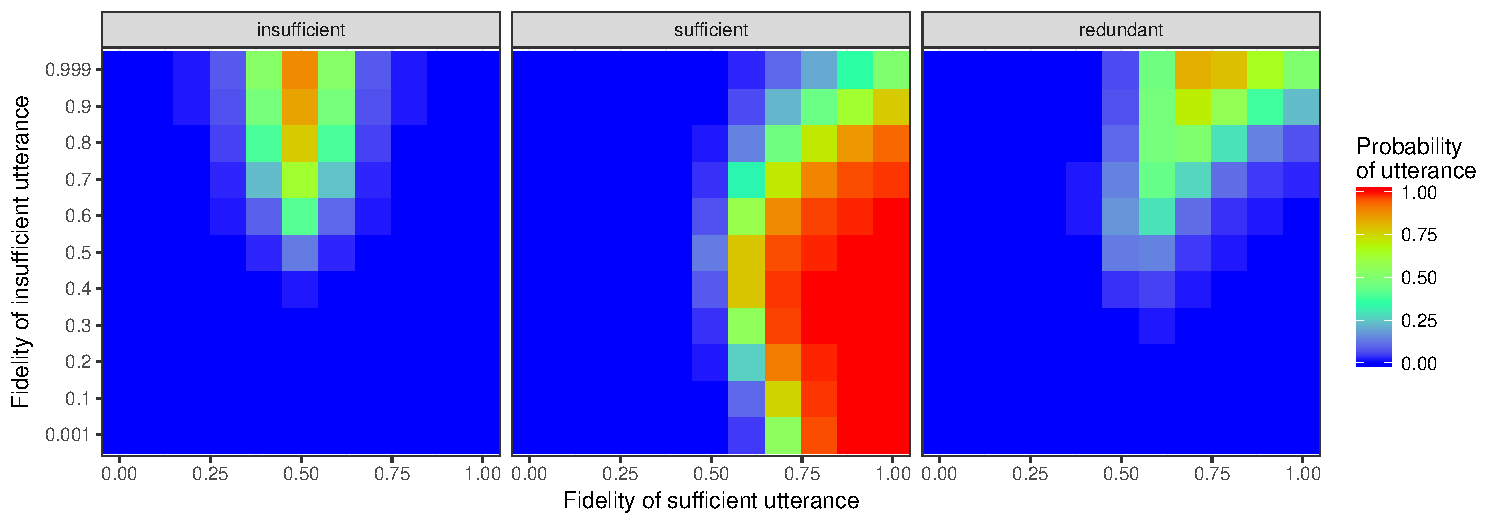
\includegraphics[width=\textwidth]{pics/modelexploration-fidelityeffect-unlogged-wide}
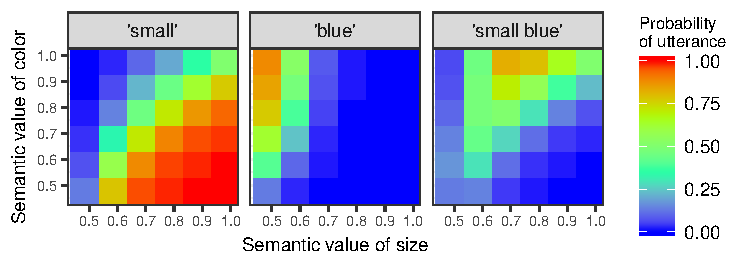
\includegraphics[width=.9\textwidth]{pics/modelexploration-fidelityeffect-paper}

\caption{Probability of producing sufficient \emph{small pin}, insufficient \emph{blue pin}, and redundant \emph{small blue pin} in contexts as depicted in \figref{fig:sizesufficient}, as a function of semantic value of color and size utterances (for $\alpha = 30$ and $ \beta_c = 0$). For a visualization of model behavior under varying $\alpha$s, see \appref{app:modelexploration}.}
\label{fig:basicasymmetry}
\end{figure}

To summarize, we have thus far shown that RSA with non-deterministic adjective semantics can give rise to the well-documented color-size asymmetry in the production of overinformative referring expressions when size adjectives are noisier than color adjectives. The crucial mechanism is this: when modifiers are noisy, adding additional, less noisy modifiers adds information. From this perspective, these redundant modifiers are not \emph{over}informative; they are rationally redundant, or sufficiently informative, given the needs of the listener. We spend the remainder of the paper demonstrating the far-reaching effects of assuming non-deterministic semantic values.

\subsection{RSA with non-deterministic semantics -- scene variation}
\label{sec:modelkoolen}

We begin by demonstrating the qualitative effect of a non-deterministic semantics on redundant referring expressions in contexts that vary in the amount of visual complexity. As discussed in \sectionref{sec:intro}, increased scene variation has been shown to increase the probability of referring expressions that are overmodified with color. Here we simulate the experimental conditions reported by \citeA{Koolen2013} and explore non-deterministic RSA's predictions for these situations. \citeA{Koolen2013}  quantified scene variation as the number of feature dimensions along which pieces of furniture in a scene varied: type (e.g., chair, fan), size (big, small), and color (e.g., red, blue).\footnote{They also included orientation (left-facing, right-facing) as a dimension along which objects could vary in certain cases. We ignore this dimension here for the sake of simplicity.} Here, we  simulate the high and low variation conditions from their Experiments 1 and 2, reproduced in \figref{fig:koolencontexts}. 

In both conditions in both experiments, color was not necessary for establishing reference; that is, color mentions were always redundant. The two experiments differed in the dimension necessary for unique reference. In Exp.~1, only type was necessary (\emph{fan} and \emph{couch} in the low and high variation conditions in \figref{fig:koolencontexts}, respectively). In Exp.~2, size and type were necessary (\emph{big chair} and \emph{small chair} in \figref{fig:koolencontexts}, respectively). \citeA{Koolen2013} found lower rates of redundant color use in the low variation conditions (4\% and 9\%) than in the high variation conditions (24\% and 18\%).

We generated model predictions for precisely these four conditions. Note that by adding the type dimension as a distinguishing dimension, we must allow for an additional semantic value $x_{\text{type}}$, which encodes how noisy nouns are.

\begin{figure}
\begin{subfigure}{.5\textwidth}
%\includegraphics[width=.9\textwidth]{pics/Koolen2013-exp1}
%\includegraphics[width=.9\textwidth]{pics/Koolen2013-exp2}
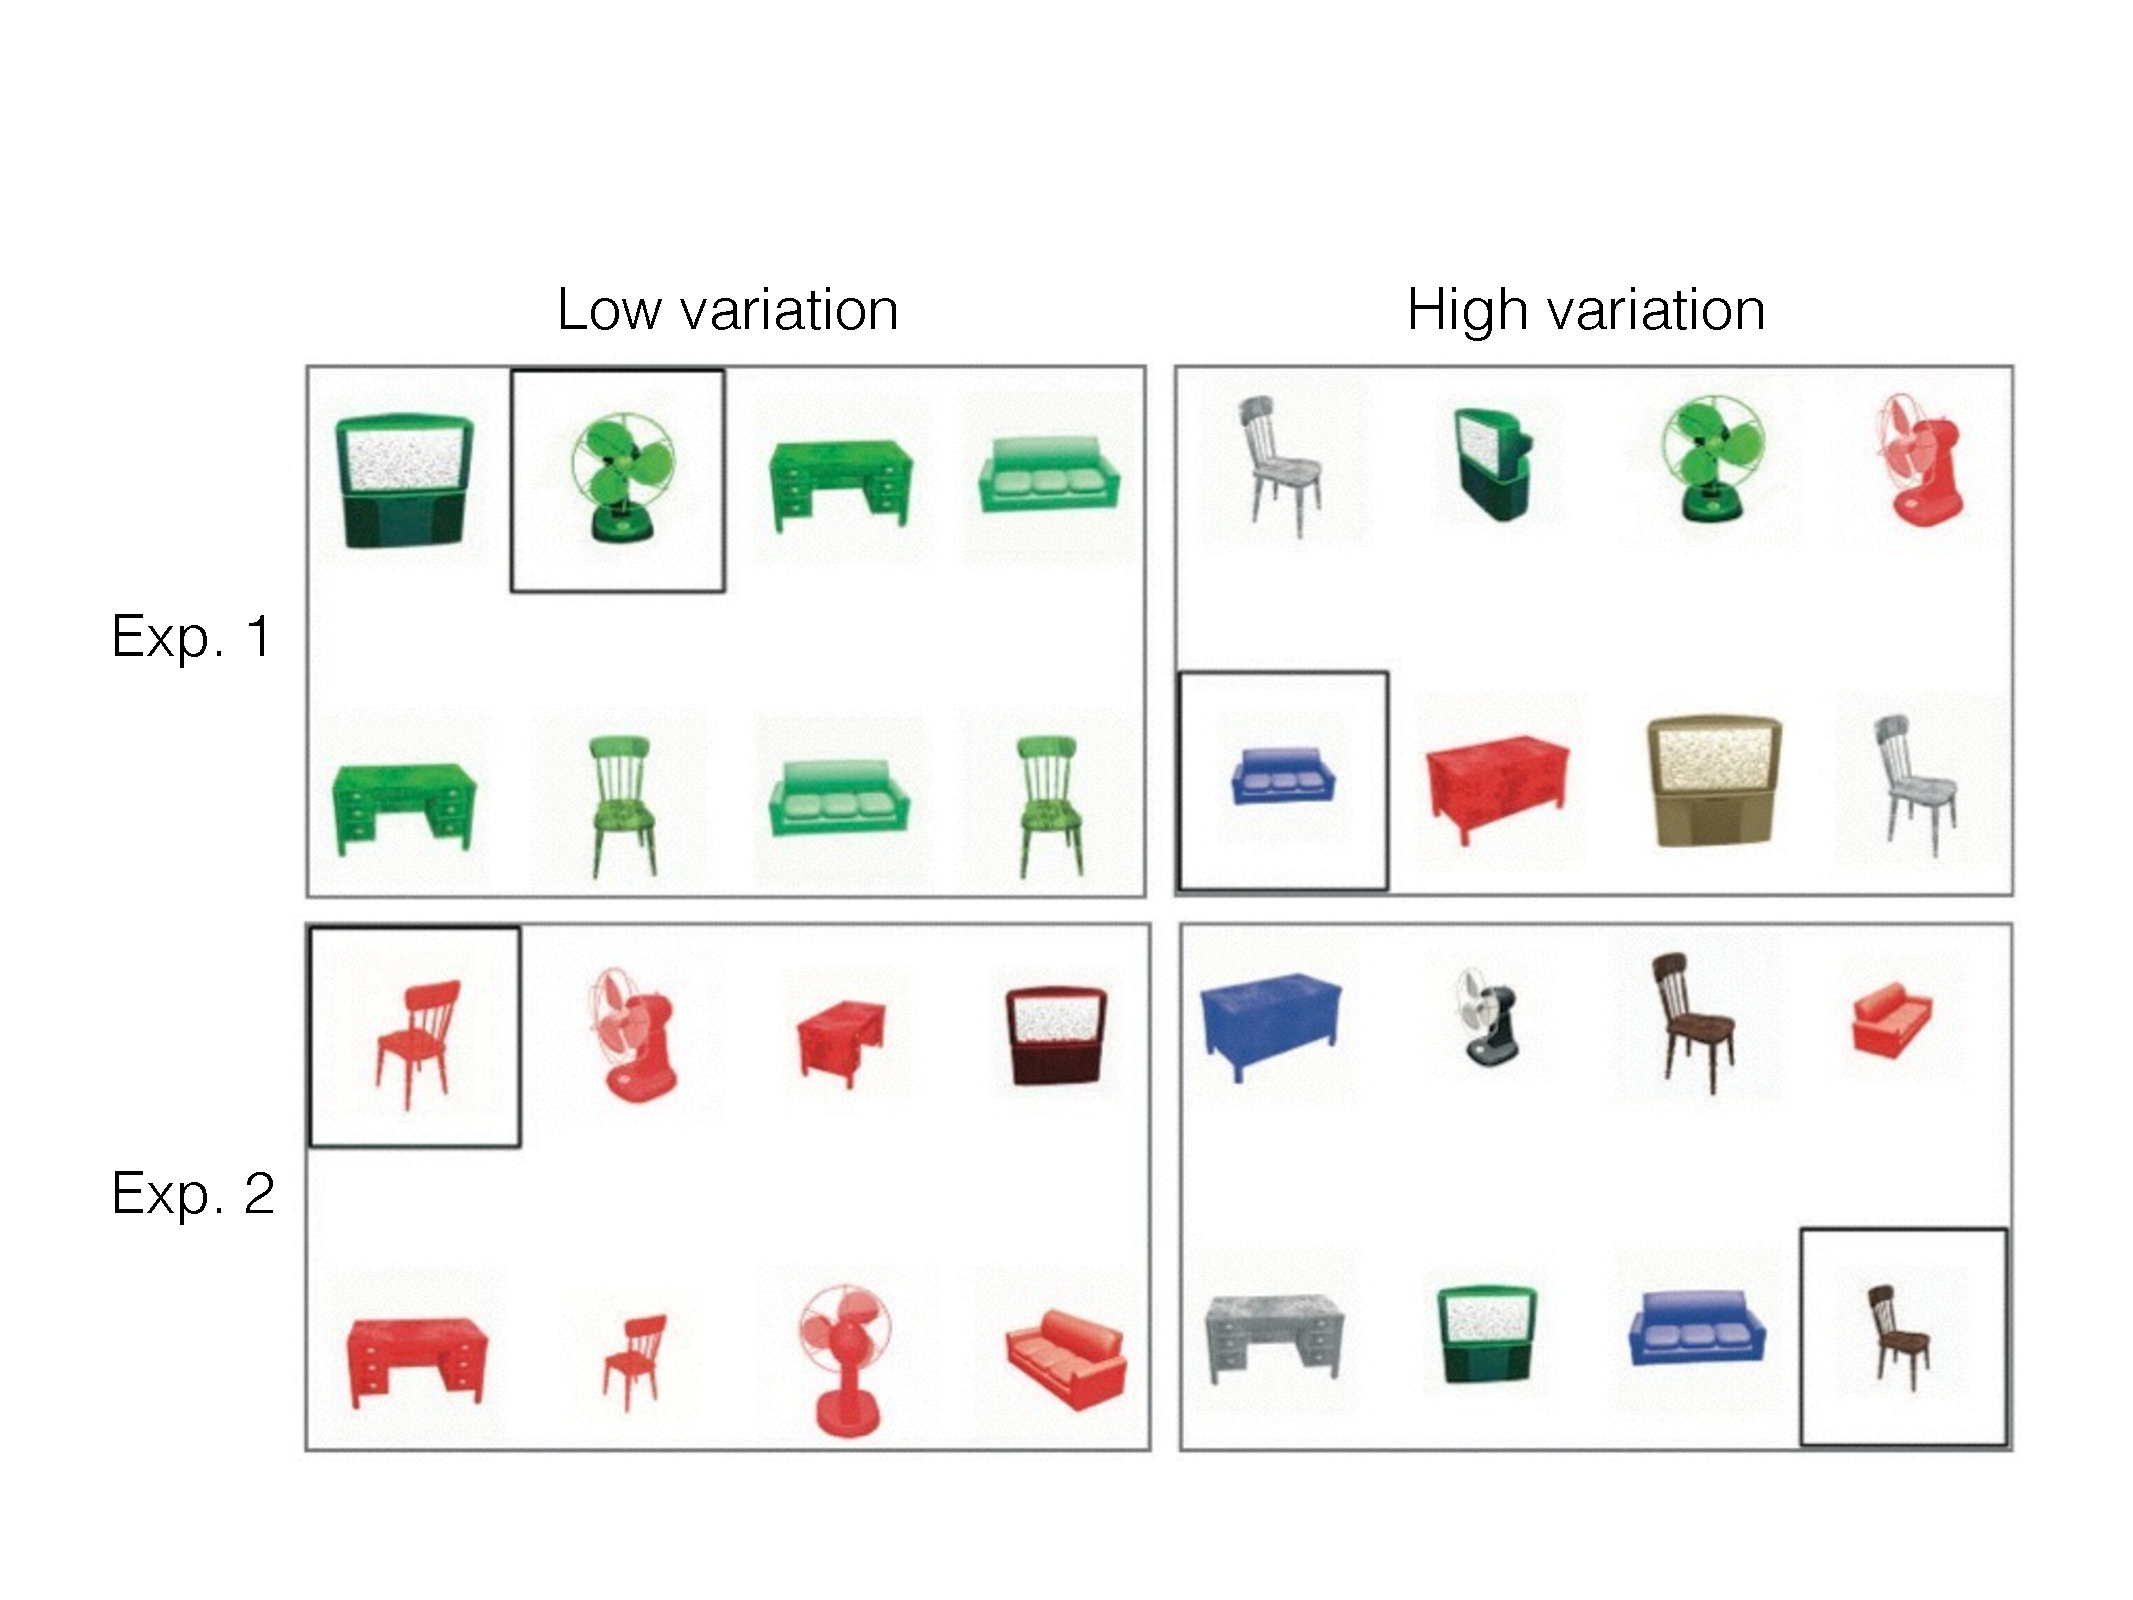
\includegraphics[width=\textwidth]{pics/koolen-conditions}
\caption{Contexts from Koolen et al.'s low variation (left column) and high variation (right column) conditions in Exp.~1 (top row) and Exp.~2 (bottom row).}
\label{fig:koolencontexts}
\end{subfigure}
\begin{subfigure}{.5\textwidth}
\centering
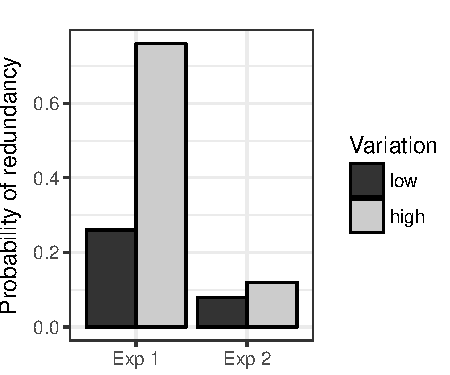
\includegraphics[width=.75\textwidth]{pics/koolen-effect}
\caption{Predicted probability of redundant color utterance in Koolen conditions for $\alpha = 30$, $ \beta_c = c(u_{\textrm{size}}) = c(u_{\textrm{color}}) = 1$, $x_{\text{size}} = .8$, $x_{\text{color}} = .999$, $x_{\text{type}} = .9$.}
\label{fig:koolensimulationresults}
\end{subfigure}
\caption{Koolen et al.~contexts and RSA model predictions.}
\end{figure}

\citeA{Koolen2013} counted any mention of color as a redundant mention. In Exp.~1, this includes the simple redundant utterances like \emph{blue couch} as well as complex redundant utterances like \emph{small blue couch}. In Exp.~2, where size was necessary for unique reference, only the complex redundant utterance \emph{small brown chair} was truly redundant.  The results of simulating these conditions for $\alpha = 30$, $ \beta_c = c(u_{\textrm{size}}) = c(u_{\textrm{color}}) = 1$, $x_{\text{size}} = .8$, $x_{\text{color}} = .999$, and $x_{\text{type}} = .9$ are shown in \figref{fig:koolensimulationresults}.%\footnote{See \appref{app:koolenexploration} for a visualization of model predictions under a fuller exploration of parameter combinations.}


For both experiments, the model retrieves the empirically observed effect of variation on the probability of redundant color mention: when variation is greater, redundant color mention is more likely. While the absolute values predicted by the model ($\approx$ 8\% to $\approx$ 75\%) are different from the values observed by \citeA{Koolen2013}  ($\approx$ 4\% to $\approx$ 24\%), it is note-worthy that non-deterministic RSA captures the qualitative scene variation effect with no further modifications.  

Differences in exact values may stem from various sources. First, the best $\alpha$ value to assume may differ from experiment to experiment. Second, semantic values may differ between experiments. Indeed, assuming a lower $x_{\text{color}}$  of .9 maintains the qualitative effects but lowers the highest probability of redundancy to .26 (which is much closer to the 24\% observed by Koolen et al). Importantly, the basic requirements to yield the empirical scene variation effect are that semantic values for size, type, and color follow the following ranking: $x_{\text{size}} \leq  x_{\text{type}} < x_{\text{color}}$. If $x_{\text{type}}$ is greater than $x_{\text{color}}$, the probability of redundantly mentioning color is close to zero and does not differ between variation conditions. This is because in those cases, color mention reduces, rather than adds, information about the target. Third, the values reported by \citeA{Koolen2013} were averaged over many different items -- here, we only reported model predictions for the example items they reported.

These results are encouraging: RSA with a non-deterministic semantics not only predicts a systematic color-size asymmetry in propensity to redundantly produce adjectives when size is noisier than color; it also predicts that there should be more redundant color mention as the number of dimensions along which objects in the scene vary increases. However, thus far we have only probed the model for qualitative effects from very few data points previously reported in the literature. Independently evaluating the utility of the model requires  testing it on large datasets. This is what we turn to next. In Sections 3, 4, and 5 we quantitatively evaluate non-deterministic RSA on datasets capturing the phenomena described in the Introduction (for a summary see \tableref{tab:effects}): modifier type and scene variation effects on modified referring expressions, typicality effects on color mention, and the choice of taxonomic level of reference in nominal choice, respectively.

\section{Non-deterministic RSA for modified referring expressions}
\label{sec:rsaevaluationbasicscene}

Adequately assessing the explanatory value of RSA with non-deterministic truth functions requires evaluating how well it does at predicting the probability of various types of utterances occurring in large datasets of naturally produced referring expressions. To this end we proceed in two steps. First we report the results of a web-based interactive reference game in which we systematically manipulate scene variation (in a somewhat different way than \citeA{Koolen2013} did). We then perform Bayesian data analysis to generate model predictions, conditioning on the observed production data. This allows us to both a) assess  how likely the model is to generate the actually observed data -- i.e., to obtain a measure of model quality -- and b) infer the posterior probability of parameter values -- i.e., to understand whether the assumed asymmetries in the adjectives' semantic values and/or cost discussed in the previous section are warranted.


\subsection{Experiment 1: scene variation in modified referring expressions}
\label{sec:exp1-scenevar}

We saw in \sectionref{sec:modelkoolen} that non-deterministic RSA correctly predicts qualitative effects of scene variation on redundant adjective use. In particular, we saw that color is more likely to be used redundantly as the number of dimensions along which objects in a scene vary increases. However, we would like to a) go beyond a qualitative investigation of scene variation effects and also b) ask whether redundant size mention is also affected by scene variation. The notion of scene variation we employ is the proportion of distractor items that do not share the value of the insufficient feature with the target, that is, as the number of distractors $n_{\textrm{diff}}$ that differ in the value of the insufficient feature divided by the total number of distractors $n_{\textrm{total}}$:

\begin{equation*}
	\textrm{scenevar} = \frac{n_{\textrm{diff}}}{n_{\textrm{total}}}
\end{equation*}

To explain, let's turn again to \figref{fig:sizesufficient}. Here, the target item is the small blue pin and there are two distractor items: a big blue pin and a big red pin. Thus, for the purpose of establishing unique reference, size is the sufficient dimension and color the insufficient dimension. There is one distractor that differs from the target in color (the big red pin) and there are two distractors in total. That is, $\textrm{scenevar} = \frac{1}{2} = .5$. Scene variation is minimal when all distractors are of the same color as the target, in which case it is 0. Scene variation is maximal when all distractors except for one (in order for the dimension to remain insufficient for establishing reference) are of a different color than the target. That is, scene variation may take on values between 0 and $\frac{n_{\textrm{total} - 1}}{n_{\textrm{total}}}$, i.e, approaching but never reaching 1.\footnote{Some readers might find this unintuitive: shouldn't scene variation be maximal when there is an equal number of same and different colors? Or when the different colors are also all different from one another? As discussed in the Introduction, there are many ways of quantifying (different aspects of) scene variation. Here we explore just one such measure; it is an interesting question whether RSA accounts equally well for different ways of quantifying scene variation. Fortunately, it is very straightforward to implement such different measures by manipulating features of distractor items and exploring the model's behavior in these contexts.}

Using the same parameter values as in the previous two model explorations ($\alpha = 30$, $ \beta_c = c(u_{\textrm{size}}) = c(u_{\textrm{color}}) = 1$, $x_{\text{size}} = .8$, $x_{\text{color}} = .999$), we generate model predictions for size-sufficient and color-sufficient contexts, varying scene variation by varying number of distractors (2, 3, or 4) and number of distractors that don't share the insufficient feature value. The resulting model predictions are shown in \figref{fig:numdistractors}: the probability of redundant adjective use increases with increasing scene variation when size is sufficient (and color redundant), but not when color is sufficient (and size redundant). This can be explained by noise distributions in the literal listener across contexts: in size-sufficient contexts, as the number of distractors of a different color than the target increases, using the relatively noiseless color term in addition to the more noisy size term reduces uncertainty about the target object more and more. However, the same is not true of the color-sufficient contexts: there is very little uncertainty about the target upon observing the minimal color utterance -- adding the size term only introduces more uncertainty about the target, regardless of the amount of scene variation. Note that this is highly dependent on the actual semantic value of color, with slightly lower semantic values for color, the model predicts small increases in redundant size use. This will be important for the interpretation of the empirical results. In general: increased scene variation is predicted to lead to a greater increase in redundant adjective use for less noisy adjectives.

\begin{figure}
\centering
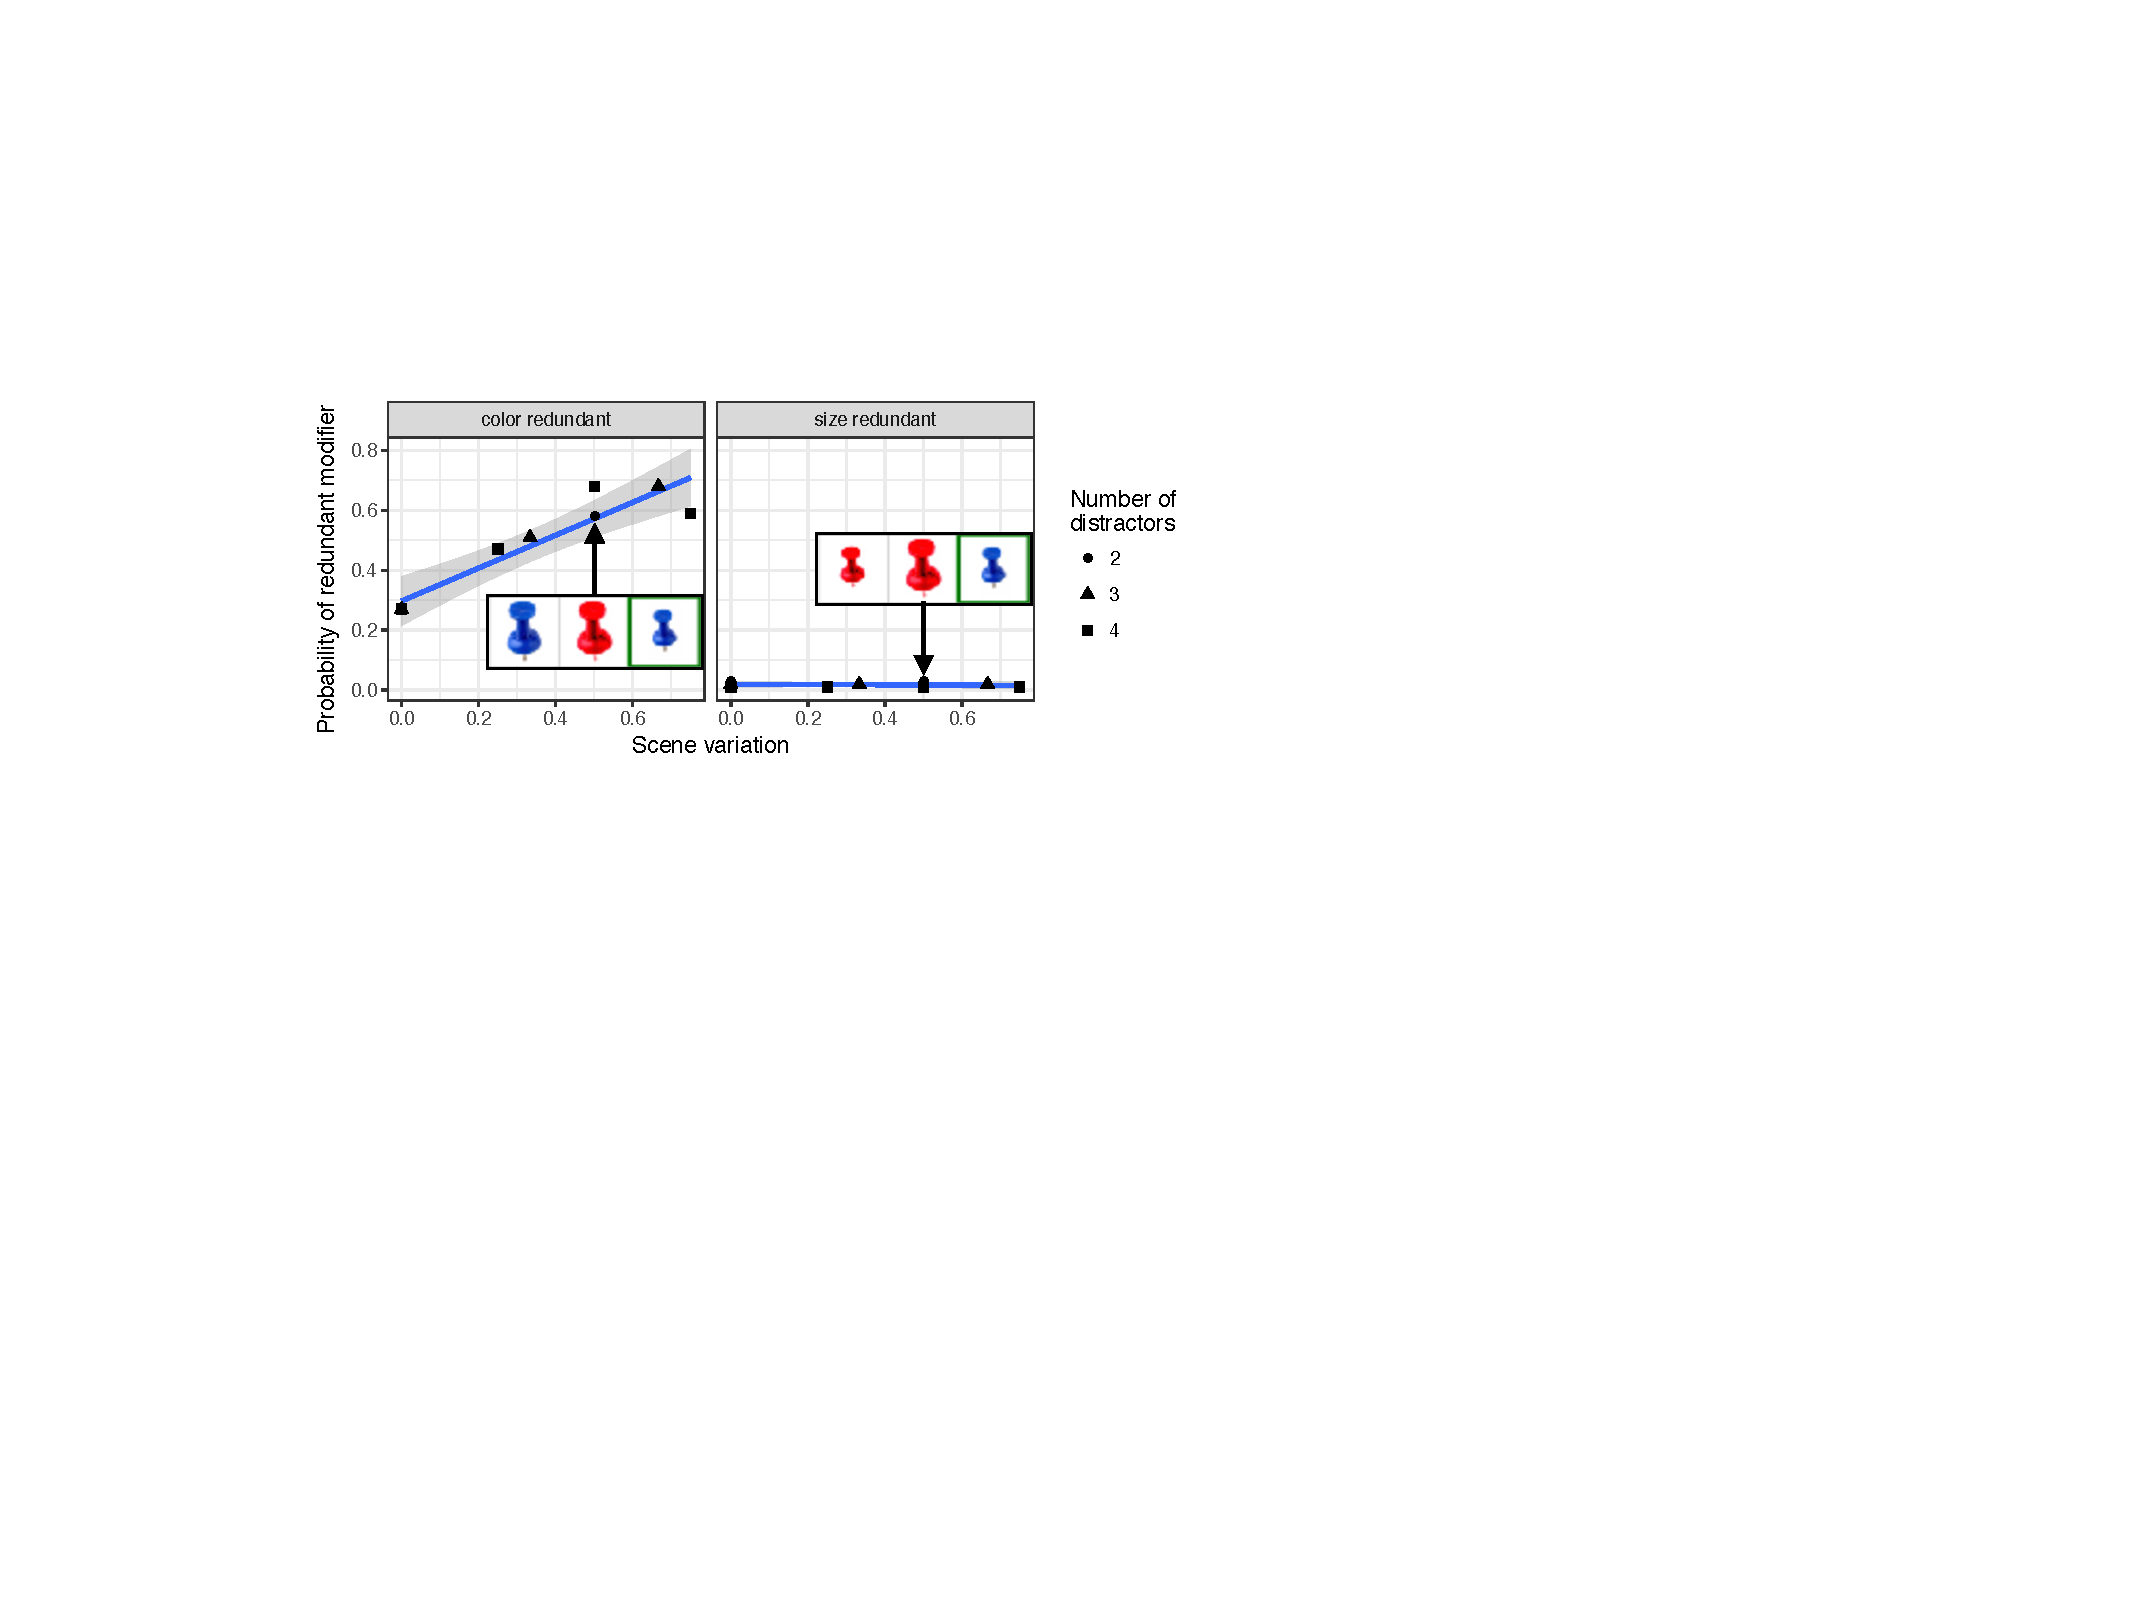
\includegraphics[width=.9\textwidth]{pics/scenevariation-annotation}
\caption{Probability of redundant utterance (\emph{small blue pin}) as a function of scene variation when size is sufficient (and color redundant, left) and when color is sufficient (and size redundant, right), for $\alpha = 30$, $ \beta_c = c(u_{\textrm{size}}) = c(u_{\textrm{color}}) = 1$, $x_{\text{size}} = .8$, $x_{\text{color}} = .999$.}
\label{fig:numdistractors}
\end{figure}


To test non-deterministic RSA predictions, we conducted an interactive web-based written production study within a reference game setting. %\footnote{See \appref{app:replication}  for a validation of the general paradigm, in which we qualitatively replicate the findings of \citeA{gatt2011} with a different set of stimuli.} 
Speakers and listeners were shown arrays of objects that varied in color and size. Speakers were asked to produce a referring expression to allow the listener to identify a target object. We manipulated the number of distractor objects in the grid, as well as the variation in color and size among distractor objects.


\subsubsection{Method}

\paragraph{Participants}

We recruited 58 pairs of participants (116 participants total) over Amazon's Mechanical Turk who were each paid \$1.75 for their participation. Data from another 7 pairs who prematurely dropped out of the experiment and who could therefore not be compensated for their work, were also included. Here and in all other experiments reported in this paper, participants' IP address was limited to US addresses and only participants with a past work approval rate of at least 95\% were accepted. 

\paragraph{Procedure}

Participants were paired up through a real-time multi-player interface \cite{Hawkins15_RealTimeWebExperiments}. For each pair, one participant was assigned the speaker role and one the listener role. They  initially received written instructions that informed participants that one of them would be the Speaker and the other the Listener. They were further told that they would see some number of objects on each round and that the speaker's task is to communicate one of those objects, marked by a green border, to the listener. They were explicitly told that using locative modifiers (like \emph{left} or \emph{right}) would be useless because the order of objects on their partner's screen would be different than on their own screen. Before continuing to the experiment, participants were required to correctly answer a series of questions about the experimental procedure. These questions are listed in \appref{app:numdistractors}.

On each trial participants saw an array of objects. The array contained the same objects for both speaker and listener, but the order of objects was randomized and was typically different for speaker and listener. In the speaker's display, one of the objects -- henceforth the \emph{target} -- was highlighted with a green border. See \figref{fig:speakerlistenerperspective} for an example of the listener's and speaker's view on a particular trial.

\begin{figure}
\begin{subfigure}{\textwidth}
\includegraphics[width=\textwidth]{pics/speaker-perspective-small.png}
\caption{Speaker's perspective.}
\label{fig:speakerpersp}
\end{subfigure}

\begin{subfigure}{\textwidth}
\includegraphics[width=\textwidth]{pics/listener-perspective-small.png}
\caption{Listener's perspective.}
\label{fig:listenerpersp}
\end{subfigure}
\caption{Example displays from the  (a) speaker's and the  (b)  listener's perspective on a \emph{size-sufficient 4-2} trial.}
\label{fig:speakerlistenerperspective}
\end{figure}

The speaker produced a referring expression to communicate the target to the listener by typing into an unrestricted chat window. After pressing Enter or clicking the `Send' button, the speaker's message was shown to the listener. The listener then clicked on the object they thought was the target, given the speaker's message.  Once the listener clicked on an object, a red border appeared around that object in both the listener and the speaker's display for 1 second before advancing to the next trial. That is, both participants received feedback about the speaker's intended referent and the listener's inference.

Both speakers and listeners could write in the chat window, allowing listeners to request clarification if necessary. Listeners could only click on an object and advance to the next trial once the speaker sent a message. 


\paragraph{Materials}

Participants proceeded through 72 trials. Of these, half were critical trials of interest and half were filler trials. On critical trials, we varied the feature that was sufficient to mention for uniquely establishing reference, the total number of objects in the array, and  the number of objects that shared the insufficient feature with the target. 

Objects varied in color and size. On 18 trials, color was sufficient for establishing reference. On the other 18 trials, size was sufficient. \figref{fig:speakerlistenerperspective} shows an example of a size-sufficient trial. We further varied the amount of variation in the scene by varying the number of distractor objects in each array (2, 3, or  4) and the number of distractors that did share the redundant feature value with the target. That is, when size was sufficient, we varied the number of distractors that shared the same color as the target. This number had to be at least one, since otherwise the redundant property would have been sufficient for uniquely establishing reference, i.e.~mentioning it would not have been redundant. Each total number of distractors was crossed with each possible number of distractors that shared the redundant property, leading to the following nine conditions: \emph{2-1, 2-2, 3-1, 3-2, 3-3, 4-1, 4-2, 4-3,} and \emph{4-4}, where the first number indicates the total number and the second number the shared number of distractors. Each condition occurred twice with each sufficient dimension. Objects never differed in type within one array (e.g., all objects are pins in \figref{fig:speakerlistenerperspective} but always differed in type across trials. Each object type could occur in two different sizes and two different colors. We deliberately chose photo-realistic objects of intuitively fairly typical colors. The 36 different object types and the colors they could occur with are listed in \appref{app:itemtypes}. 


Fillers were target trials from Exp.~2, a replication of \citeA{GrafEtAl2016}. Each filler item contained a three-object grid. None of the filler objects occurred on target trials. Objects stood in various taxonomic relations to each other and required neither size nor color mention for unique reference. See \sectionref{sec:exp2} for a description of these materials.

\subsubsection{Data pre-processing and exclusion}

We collected data from 2171 critical trials. Because we did not restrict participants' utterances in any way, they produced many different kinds of referring expressions. Testing the model's predictions required, for each trial, classifying the produced utterance as an instance of a \emph{color}-only mention, a \emph{size}-only mention, or a \emph{color-and-size} mention (or excluding the trial if no classification was possible). To this end we conducted the following semi-automatic data pre-processing. 

%In a first step, an R script automatically checked whether (what the experimenters deemed to be) the target's color or size was included in the utterance. In this way, \red{XXX \%} of cases were classified as containing a size or color term. However, this did not capture that sometimes, a participant produced a different color or size term than the one we had intended (e.g., \emph{pink} instead of \emph{purple} \red{XXX \%} or \emph{large} instead of \emph{big} \red{XXX \%}) or the expression contained a typo (e.g., \emph{pruple} instead of \emph{purple} \red{XXX \%}). In a second step, one of the authors (CG) therefore manually checked the automatic coding: utterances of an unintended color or size were coded as an instance of the intended color or size if they were similar enough in meaning and utterances with typos were corrected. Most of the time, participants converged on a convention of mentioning simply the target's size and/or color, e.g., \emph{purple} or \emph{big blue}, without even using an article (e.g., \emph{the}) or mentioning the object's type (e.g., \emph{comb}). Articles were omitted in 93.2 \% of cases and object types were omitted in 74.2 \% of cases. We did not analyze this any further.

First, 33 trials on which the listener selected the wrong referent were excluded, leading to the elimination of 1.5\% of trials. Then, an R script automatically checked whether the speaker's utterance contained a precoded color (i.e. \emph{black, blue, brown, gold, green, orange, pink, purple, red, silver, violet, white, yellow}) or size (i.e. \emph{big, bigger, biggest, huge, large, larger, largest, little, small, smaller, smallest, tiny}) term. In this way, 95.7 \% of cases were classified as mentioning size and/or color. However, this did not capture that sometimes, participants produced meaning-equivalent modifications of color/size terms for instance by adding suffixes (e.g., \emph{bluish}), using abbreviations (e.g., \emph{lg} for \emph{large} or \emph{purp} for \emph{purple}), or using non-precoded color labels (e.g., \emph{lime} or \emph{lavender}). Expressions containing a typo (e.g., \emph{pruple} instead of \emph{purple}) could also not be classified automatically. In the next step, one of the authors (CG) therefore manually checked the automatic coding to include these kinds of modifications in the analysis. This covered another 1.5\% of trials. Most of the time, participants converged on a convention of producing only the target's size and/or color, e.g., \emph{purple} or \emph{big blue}, but not an article (e.g., \emph{the}) or the noun corresponding to the object's type  (e.g., \emph{comb}). Articles were omitted in 93.1 \% of cases and nouns were omitted in 71.5 \% of cases. We did not analyze this any further.

There were 50 cases (2.3\%) in which the speaker made reference to the distinguishing dimension in an abstract way, e.g.~\emph{different color}, \emph{unique one}, \emph{ripest}, \emph{very girly}, or \emph{guitar closest to viewer}. While interesting as utterance choices,\footnote{Certain participants seemed to have deliberately used this as a strategy even though simply mentioning the distinguishing property would have been shorter in most cases. In all, only 12 participants produced these kinds of utterances: one 18 times, one 8 times, one 6 times, two 3 times, one 2 times, and the remaining six only once each.} these cases were excluded from the analysis. There were 3 cases that were nonsensical, e.g. \emph{bigger off a shade}, which were also excluded. Finally, there were 6 cases where only the insufficient dimension was mentioned -- these were excluded from the analysis reported in the next section, where we are only interested in minimal or redundant utterances, not underinformative ones, but were included in the Bayesian data analysis reported in \sectionref{sec:modifiermodeleval}. After the exclusion, 2079 cases classified as one of \emph{color}, \emph{size}, or \emph{color-and-size} entered the analysis.

%\jd{Caroline, is there anything else we should mention here?}caroline:Should we mention that we included lighter/darker mentions as color mentions? (There are ~10; especially used to describe turtles and avocados)

\subsubsection{Results}
\label{sec:modelempiricalresults}
% The analysis R script is in writing/2016/theory/rscripts/analysis_modifiers.R

Proportions of redundant \emph{color-and-size} and minimal \emph{color} or \emph{size} utterances are shown in \figref{fig:exp1results} alongside model predictions (to be explained further in \sectionref{sec:modifiermodeleval}). There are three main questions of interest: first, do we replicate the color/size asymmetry in probability of redundant adjective use? Second, do we replicate the previously established effect of increased redundant color use with increasing scene variation? Third, is there an effect of scene variation on redundant size use and if so, is it smaller compared to that on color use, as is predicted under asymmetric semantic values for color and size adjectives?

We addressed all of these questions in one fell swoop by conducting a mixed effects logistic regression analysis predicting redundant over minimal adjective use from fixed effects of sufficient property (color vs.~size), scene variation (proportion of distractors that does not share the insufficient property value with the target), and the interaction between the two.\footnote{All mixed effects analyses reported in this paper were conducted with the \verb+lme4+ package \cite{lme4} in R \cite{R}.} The model included the maximal random effects structure that allowed the model to converge: by-speaker and by-item random intercepts as well as by-speaker random slopes for scene variation. 

We observed a main effect of sufficient property, such that speakers were more likely to redundantly use color than size adjectives ($\beta = 3.61$, $SE = .23$, $p < .0001$), replicating the much-documented color-size asymmetry. We further observed a main effect of scene variation, such that redundant adjective use increased with increasing scene variation ($\beta = 4.11$, $SE = .49$, $p < .0001$). Finally, we also observed a significant interaction between sufficient property and scene variation ($\beta = 3.03$, $SE = .81$, $p < .0002$). Simple effects analysis revealed that the interaction was driven by the scene variation effect being much smaller in the \emph{color-sufficient} condition ($\beta = 2.59$, $SE = .78$, $p < .0009$) than in the \emph{size-sufficient} condition ($\beta = 5.63$, $SE = .45$, $p < .0001$), as predicted if size modifiers are noisier than color modifiers.



\begin{figure}
\centering
%\includegraphics[width=\textwidth]{../../../models/1a_bda_basic/results_bda/graphs/scenevariation-fixed-reducedconditions}
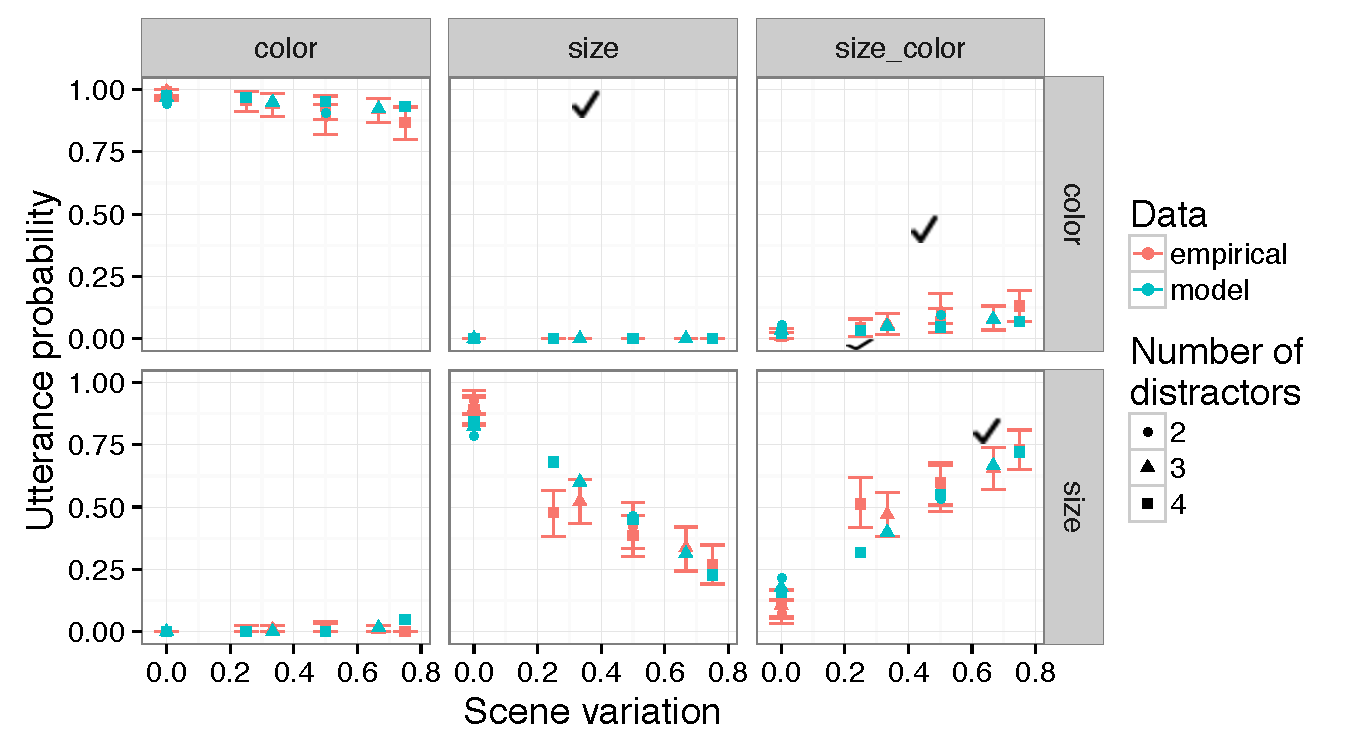
\includegraphics[width=\textwidth]{../../../models/old/1a_bda_basic/results_bda/graphs/scenevariation-fixed-reducedconditions-unlogged}
\caption{Empirical utterance proportions  (red)  alongside point-wise maximum a posteriori (MAP) estimates of the RSA model's posterior predictives for utterance probability (blue) as a function of scene variation. Rows indicate the sufficient dimension, columns the produced utterance. Here and in all following plots, error bars indicate 95\% bootstrapped confidence intervals.}
\label{fig:exp1results}
\end{figure}


\subsection{Model evaluation: scene variation}
\label{sec:modifiermodeleval}

% Extra info: 10000 samples, burn 3000, uniform drift, acceptance rate .4

In order to evaluate RSA with non-deterministic truth functions, we asked how well it captures the empirical data. To this end we conducted a Bayesian Data Analysis. \jd{Robert, can you insert 1-2 more sentences here that capture the essence of BDA?} This allowed us to  simultaneously generate model predictions and infer likely parameter values, by conditioning on the observed production data (coded into \emph{size}, \emph{color}, and \emph{size-and-color} utterances as described above) and integrating over the following free parameters: semantic value for color $x_{\textrm{color}}$, semantic value for size $x_{\textrm{size}}$, color cost $c(u_{\textrm{color}})$, size cost $c(u_{\textrm{size}})$, cost weight $\beta_c$, and speaker rationality parameter $\alpha$. We assumed uniform priors for each parameter: $x_{\textrm{color}} \sim \mathcal{U}(0,1)$, $x_{\textrm{size}} \sim \mathcal{U}(0,1)$, $c(u_{\textrm{color}}) \sim \mathcal{U}(0,2)$, $c(u_{\textrm{size}}) \sim \mathcal{U}(0,2)$, $\beta_c \sim \mathcal{U}(0,10)$, $\alpha  \sim \mathcal{U}(0,40)$.
Inference for the cognitive model was exact. We used Markov Chain Monte Carlo (MCMC) to infer posteriors for the six free parameters.

Point-wise maximum a posteriori (MAP) estimates of the model's posterior predictives for each combination of utterance, sufficient dimension, number of distractors, and number of different distractors (collapsing across different items) are compared to empirical data in \figref{fig:modelexp1scatter}. At this level, the model achieves a correlation of $r = .99$. Looking at results additionally on the by-item level yields a correlation of $r = .85$. The model thus does a very good job of capturing the quantitative patterns in the data. This can also be seen in \figref{fig:exp1results}, where model predictions are plotted alongside the empirical proportions by condition. The only clear flaw is that the model predicts greater redundant adjective use than empirically observed when there is no scene variation at all. \jd{Noah, can you add a sentence on why, given that you've thought about this for the negation case as well?}.

\begin{figure}
\centering
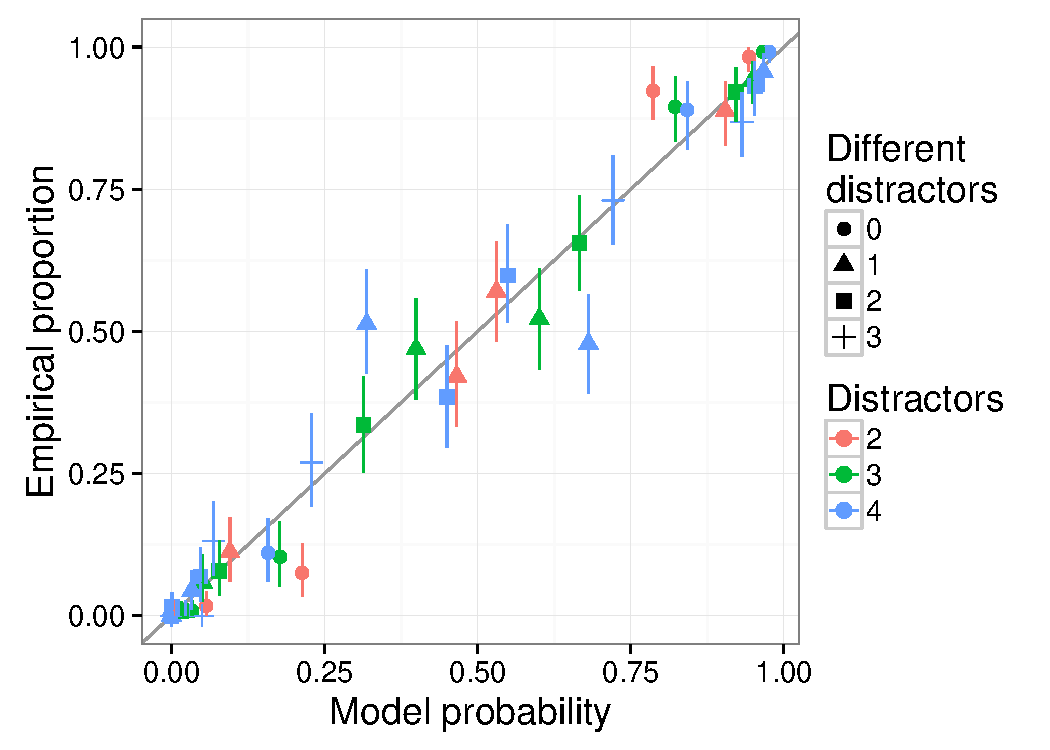
\includegraphics[width=.8\textwidth]{../../../models/old/1a_bda_basic/results_bda/graphs/predictives-collapsed-fixed-reducedconditions-unlogged}
\caption{Scatterplot of point-wise maximum a posteriori (MAP) estimates of the RSA model's posterior predictives against empirical proportions ($r=$.85). \jd{update this plot once bda run}}
\label{fig:modelexp1scatter}
\end{figure}

Parameter posteriors are shown in \figref{fig:modifierparamposteriors}. Crucially, the semantic value of color is inferred to be higher than that of size -- there is no overlap between the 95\% highest density intervals (HDIs) for the two parameters. That is, size modifiers are inferred to be noisier than color modifiers. The relatively high inferred $\alpha$ suggests that this difference in semantic value contributes substantially to the observed color-size asymmetries in redundant adjective use. As for cost, there is a lot of overlap in the inferred cost of size and color modifiers, suggesting that no cost difference is necessary to obtain the color-size asymmetry and the scene variation effects. These results are compatible with previous claims \red{cite cite} that part of the explanation for the color-size asymmetry stems from the low cognitive cost involved in producing color modifiers compared to size modifiers. However, the results do suggest that a cost asymmetry is not the driving force behind the asymmetry in redundant adjective use. Note further that the asymmetry cannot be reduced to cost differences: in \sectionref{sec:modifiedmodel} we showed that the color-size asymmetry in redundant adjective use requires an asymmetry in modifier fidelity. An asymmetry in cost only serves to further enhance the asymmetry brought about by the fidelity asymmetry, but cannot carry the redundant use asymmetry on its own.
%\red{the following cost discussion is deprecated and applies only to logged fidelities} As for cost, the cost of size modifiers is inferred to be roughly twice that of color, with a non-zero inferred weight on cost. This provides some support for previous claims \red{cite cite} that part of the explanation for the color-size asymmetry stems from the low cognitive cost involved in producing color modifiers compared to size modifiers. However, note that the asymmetry cannot be reduced to cost differences: indeed in \sectionref{sec:modifiedmodel} we showed that the color-size asymmetry in redundant adjective use requires an asymmetry in modifier fidelity. An asymmetry in cost only serves to further enhance the asymmetry brought about by the fidelity asymmetry, but cannot carry the redundant use asymmetry on its own.


\begin{figure}
\centering
%\includegraphics[width=\textwidth]{../../../models/1a_bda_basic/results_bda/graphs/parameterposteriors-fixed-reducedconditions}
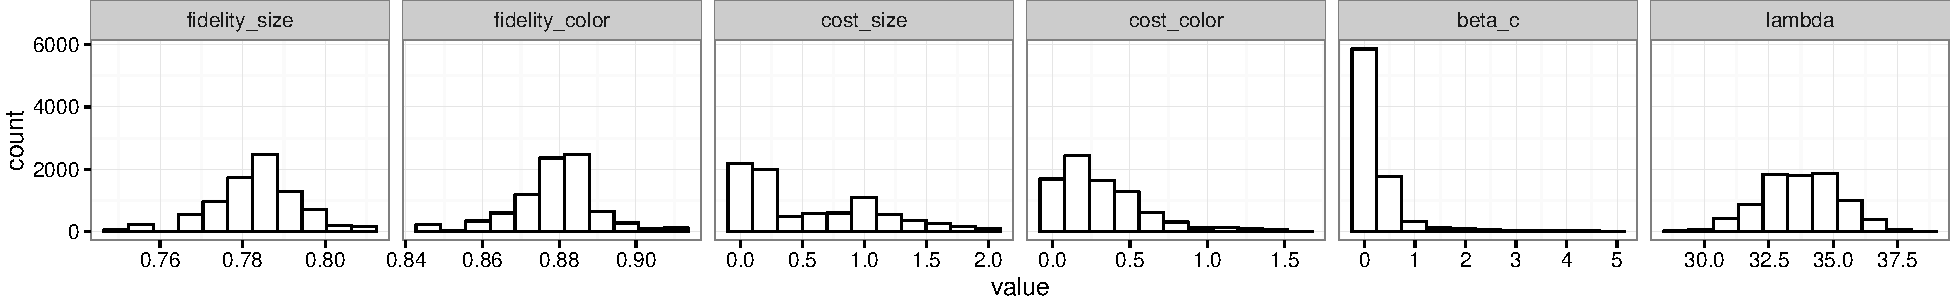
\includegraphics[width=\textwidth]{../../../models/old/1a_bda_basic/results_bda/graphs/parameterposteriors-fixed-reducedconditions-unlogged}
\caption{Posterior distribution over model parameters. Maximum a posteriori (MAP)  $f_{\textrm{s}}$ = 0.79, 95\% highest density interval (HDI) = [0.76,0.80]; MAP $f_{\textrm{c}}$ = 0.88, HDI = [0.86,0.91]; MAP $c_{\textrm{size}}$ = .08, HDI = [0, 1.5]; MAP $c_{\textrm{color}}$ = 0.07, HDI = [0,0.9]; MAP $\beta_c$ = 0.04, HDI = [0,1.6]; MAP $\alpha$ = 34.0, HDI = [30.8,36.5] \jd{update this plot once new bda run}}
\label{fig:modifierparamposteriors}
\end{figure}

\subsection{Discussion}
\label{sec:modifierdiscussion}

In this section, we reported the results of a dataset of freely collected referring expressions that replicated the well-documented color-size asymmetry in redundant adjective, the effect of scene variation on redundant color use, and showed a novel effect of scene variation on redundant size use. We also showed that non-deterministic RSA provides an excellent fit to these data. In particular, the crucial element in obtaining the color-size asymmetry is that size adjectives be noisier than  color adjectives, capture in RSA via a lower semantic value for size compared to color. Asymmetries in cost of adjectives  only serve to further enhance the modification asymmetry resulting from the asymmetry in semantic value. In addition, we showed that asymmetric effects of scene variation on overmodification are also well captured by non-deterministic RSA: scene variation leads to a greater increase in overmodification with less noisy than with more noisy modifiers. \jd{this is very cool -- can someone more american than me please express this here?}

Some readers may find themselves wondering about the status of these semantic values: are we claiming that color modifiers have inherently higher semantic values than size modifiers? Is the difference constant? What if the color modifier is a less well known one like \emph{mauve}? The way we have set the model up thus far, there would indeed be no difference in semantic value between \emph{red} and \emph{mauve}. Moreover, the model is not equipped to handle potential object-level idiosyncracies such as the typicality effects discussed in \sectionref{sec:colortypicalityintro}. We defer a fuller discussion of the status of the semantic value term to the General Discussion and turn first to non-deterministic RSA's potential for capturing these typicality effects.


\section{Feature typicality}
\label{sec:colortypicality}

\jd{rewrite this intro once settled on whether or not we'll use continuous semantics as oppposed to truth-conditional  plus noise from the start?}

In \sectionref{sec:rsaevaluationbasicscene} we showed that non-deterministic RSA successfully captures both the basic asymmetry in overmodification with color vs.~size as well as effects of scene variation, quantified in various different ways. But in \sectionref{sec:colortypicalityintro} we discussed a further characteristic of speakers' overmodification behavior: speakers are more likely to redundantly produce modifiers that denote atypical rather than typical object features, i.e., they are more likely to refer to a blue banana as a \emph{blue banana} rather than as a \emph{banana}, and they are more likely to refer to a yellow banana as a \emph{banana} than as a \emph{yellow banana} \cite{sedivy2003a, Westerbeek2015}. Non-deterministic RSA as we have set it up thus far does not capture this asymmetry: it knows that a particular modifier is a color modifier with a particular fidelity; it does not know anything about the typicality of the denoted properties for the referent. 

We would like to warn and disillusion the reader upfront: we will not solve the problem of how to get overmodification behavior from the typicality of features compositionally. This is a problem for all theories of modification \cite{kamp1995}. However, we would like to offer a proof of concept showing that, if the non-determinism in the RSA semantics is not at the adjective type (color, size) level, but instead at the level of combinations of referring expressions and objects, the model produces precisely the sorts of typicality effects reported in the literature. 

Let us elaborate. Where before we took a fidelity to be a number between 0 and 1 indicating how likely a type of modifier (size, color) was to correctly apply to an object, we now treat it as indicating how good an instance of a particular referring expression the object in question is. For example, take the banana case: assume three contexts of objects with yellow, brown, and blue objects. Assume further that one of the objects is a banana, and the only difference between the three contexts is whether the banana is blue, brown, or yellow. In every context there is another object of the same color as the banana, so color is redundant, while there are no other bananas, so object category mention is sufficient for reference. Assume further the fidelity values shown in \tableref{tab:colorobjectfidelities}. These values should be read as follows: a yellow banana is a very good or typical instance of a\emph{banana} -- \emph{banana} applied to yellow bananas has a high fidelity of .9. In contrast, brown bananas are less typical instances of \emph{banana}s (.35), and blue bananas are highly atypical \emph{banana}s (.1) but still better than objects of an other non-banana type (.015). Going along the diagonal, you can see that we assume for each remaining utterance that its fidelity is very high (.99) when applied to an object in its extension and very low otherwise (.015).

\begin{table}
\centering
\caption{Hypothetical fidelity values for utterances (rows) as applied to objects (columns).}
\begin{tabular}{l l l l l}
\toprule
Utterance & yellow banana & brown banana & blue banana & other\\
\midrule
\emph{banana} & .9 & .35 & .1 & .015 \\
\emph{yellow banana} & .99 & .015 & .015 & .015 \\
\emph{brown banana} & .015 & .99 & .015 & .015 \\
\emph{blue banana} & .015 & .015 & .99 & .015 \\
\emph{other} & .015 & .015 & .015 & .99 \\
\bottomrule
\end{tabular}
\label{tab:colorobjectfidelities}
\end{table}

With $\alpha$ = 12 and $\beta_c$ = 5 (that is, both informativeness and utterance cost receive a substantial weight), the resulting speaker probabilities for the (minimal) \emph{banana} are .99, .37, and .05, respectively, to refer to the yellow banana, the brown banana, and the blue banana. In contrast, the resulting speaker probabilities for the redundant \emph{yellow banana}, \emph{brown banana}, and \emph{blue banana} are .01, .63, and .95, respectively. That is, redundant color mention increases with decreasing fidelity of the simple \emph{banana} utterance.

So far we have shown that non-deterministic RSA can capture typicality effects in principle if we assume that fidelity does not operate at the adjective type level but instead captures the typicality of an object for the alternative (minimal and redundant) referring expressions. If an object is more typical for the redundant expression than for the minimal expression, then the bigger the difference in typicality, the greater the relative informativeness of the redundant expression, and the greater the probability of it being produced. This is related to Levinsonian stereotype inferences \cite{levinson2000}: the speaker reasons that just saying \emph{banana} will lead a listener to believe they are referring to a  stereotypical instance of banana (i.e., a yellow one). In order to prevent this (incorrect) stereotype inference they add a modifier to refer to the blue one.

We can now ask whether taking into account this more fine-grained notion of a non-deterministic semantics affects the probability of redundantly mentioning color. Because the stimuli for Exp.~1 were specifically designed to be realistic objects with low color-diagnosticity, they do not include objects with low typicality values or large degrees of variation in typicality. \jd{note that to the extent that there is variation, we do see typicality effects, but they are small} This makes the dataset from Exp.~1 not well-suited for investigating typicality effects. We therefore conducted a separate production experiment in the same paradigm but with two broad changes: first, objects' color varied in typicality; and second, we did not manipulate object size, focusing only on color mention. This allows us to ask two question: first, do we replicate the typicality effects reported in the literature -- that is, are less typical objects more likely to lead to redundant adjective use than more typical objects? Second, does RSA with empirically elicited typicality values as proxy for a continuous semantics capture speakers' behavior better than just typicality alone? 

\jd{foreshadow the informativeness conditions}

\subsection{Experiment 2: Color typicality effects}
\label{sec:modifiertypicalityeffects}

\begin{figure}
	\centering
	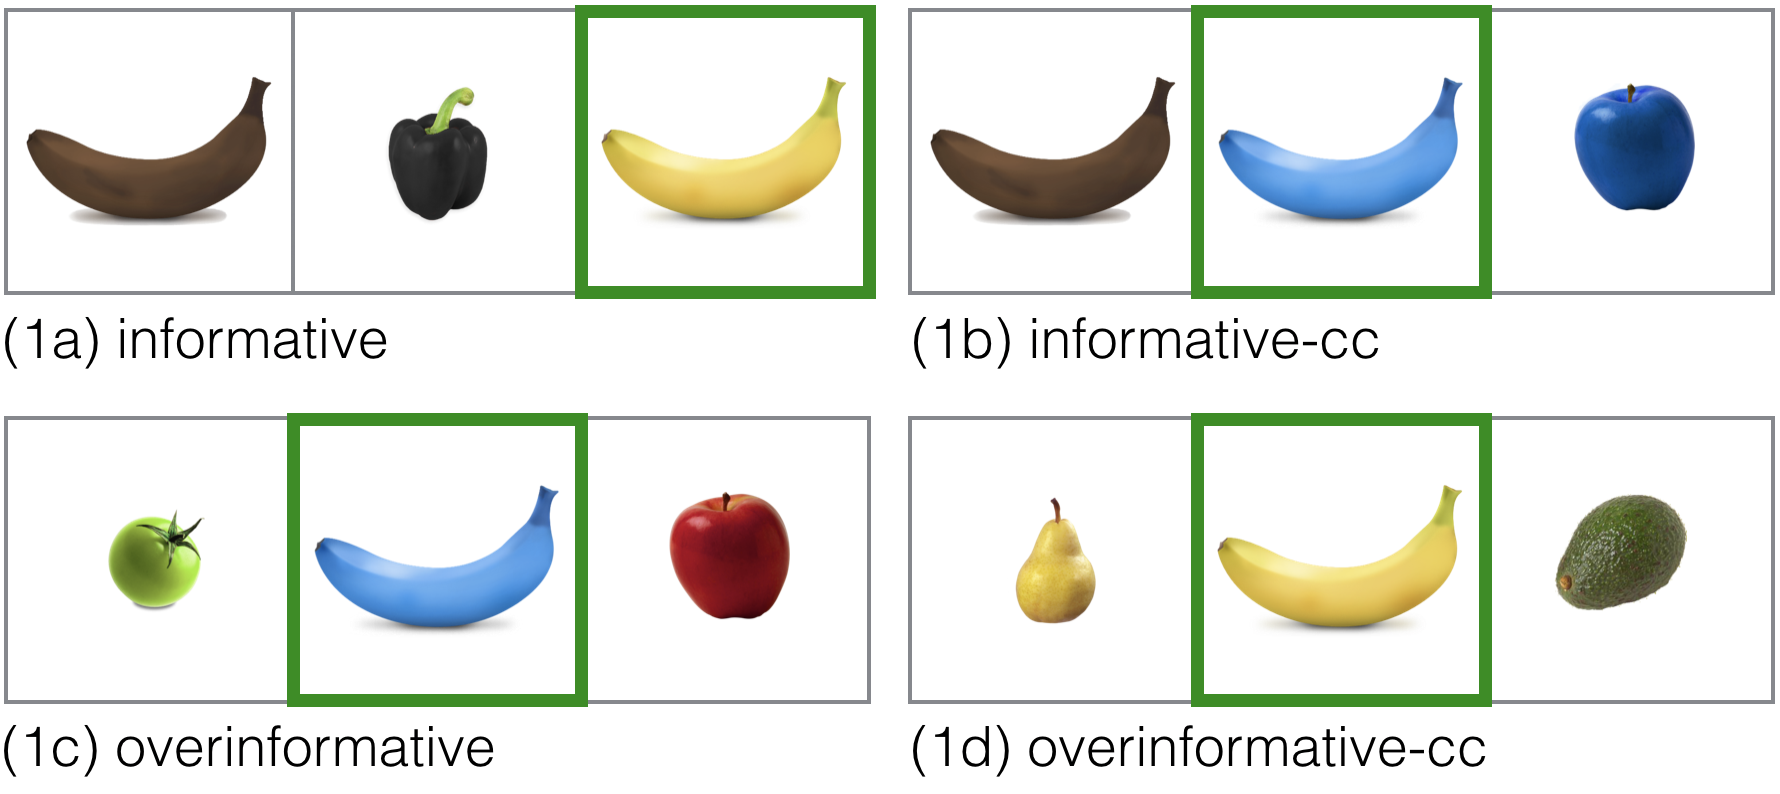
\includegraphics[width=.5\textwidth]{pics/context_overview}
	\caption{The four context conditions, exemplified by the \textit{banana} domain. The target is outlined in green; the color and type of the distractors differ with each condition (see text). \jd{elisa: please make this figure with exactly the same labels as in  results Figure 4 (informative, informative-cc, etc, and explain in figure caption -- in making labels shorter, also make them more legible or we'll be rejected outright for illegible figures.}
	}
	\label{fig:contexts}
\end{figure}

\begin{figure}[bt!]
	\centering
	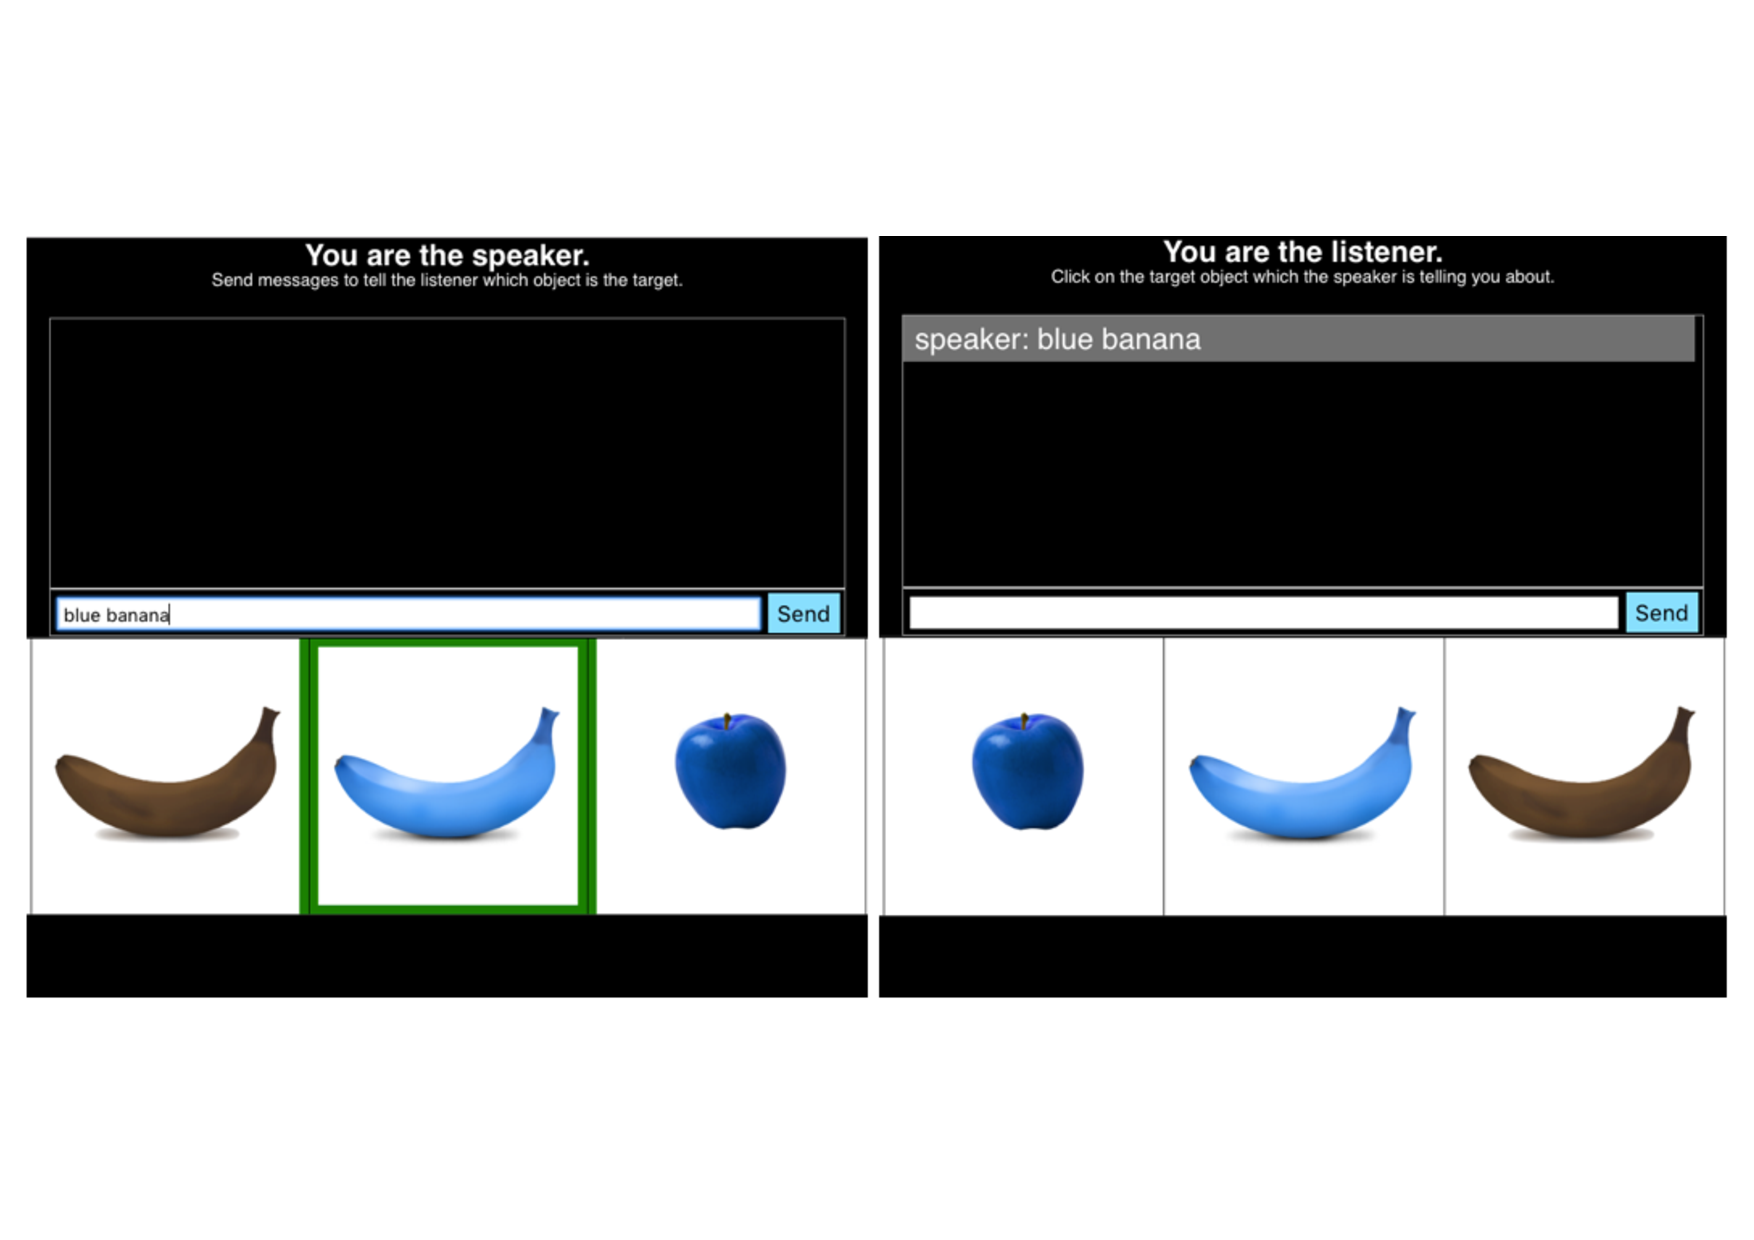
\includegraphics[width=.5\textwidth]{pics/design_0}
	\caption{Experimental setup.
	}
	\label{fig:mturk}
\end{figure}

\subsubsection{Methods}

\paragraph{Participants}

We recruited 120 self-reported native speakers of English over Mechanical Turk \jd{who bla}. 

\paragraph{Procedure and materials}

The procedure was identical to that of Exp.~1. 

On each trial, exactly three objects were displayed. The stimuli were selected from seven food items (apple, avocado, banana, carrot, pear, pepper, tomato) which each occurred in three different colors that intuitively differed in typicality for that item. For example, the banana occurred in the colors yellow, brown, and blue. Each item occurred as a target and as a distractor. A pepper additionally occurred in a fourth color which only functioned as a distractor due to the need for a green color competitor.

%\paragraph{\bf Design}
Each presented context consisted of three objects, one target and two distractors. The contexts always corresponded to one out of four possible conditions. The different context conditions are referred to as ``informative without a color competitor" (\figref{fig:contexts}a), ``informative with a color competitor" (\figref{fig:contexts}b), ``overinformative without a color competitor" (\figref{fig:contexts}c), and ``overinformative with a color competitor" (\figref{fig:contexts}d). A context is referred to as overinformative when mentioning the type of the item, e.g., banana, would be sufficient for an unambiguous identification of the target. An additional mention of color would mean that the speaker uses the color adjective overinformatively, i.e., they are adding ``unnecessary" information. However, in this condition the target never has a color competitor, i.e., if the target is brown, there is no distractor of the same color in the context. This means that an only-color utterance would lead to an unambiguous identification, too. This is not possible in the overinformative condition with a color competitor (Fig.~1d). In the informative conditions, the speaker needed to mention the color in addition to the type to provide an unambiguous utterance. Again, one context type did (Fig.~1a) and one did not include a color competitor among its distractors (Fig.~1b).

The item selection was randomized but conditioned on the corresponding context condition, i.e., the items had to fulfill the properties dictated by the condition. In the end, each participant saw 42 different contexts. All of the differently colored items were the target exactly twice but the context in which they occurred was drawn randomly from the four possible conditions mentioned above. All in all, there were 84 different configurations, i.e., seven target food items, each of them in three colors, where each could occur in four contexts. Trial order was randomized.


\subsubsection{Annotation and exclusions}
After collecting the data, the different utterances were automatically  labeled as belonging to one of the following categories: type-only ("banana"), color-and-type ("yellow banana"),  color-only ("yellow"), category-only ("fruit"), color-and-category ("yellow fruit"), description ("has green stem"), color-modifier ("funky carrot"), and negation ("yellow but not banana"). Two participants were excluded because they did not finish the experiment. Trials on which the speaker did not produce any utterances and trials on which the listener did not identify the target correctly were excluded as well. The remaining utterances (94\% of the original set) were cleaned manually for misspellings and abbreviations, e.g., ``banan'' for banana. Finally, there were 10 speakers who consistently used roundabout descriptions instead of direct referring expressions (e.g., ``monkeys love\dots'' for banana). These participants were excluded because they were not trying to communicate the target, but rather appeared to be playing the game of Taboo.

The 1942 resulting utterances were then categorized according to the categories laid out above. Only five utterances (0.003\%) were assigned to the category "other".


\subsubsection{Typicality norming}

\jd{make this more structured, ie change from cogsci paper prose}
To evaluate the model, we collected empirical typicality values for each utterance-object pair. Ratings were collected across three separate studies. The first study collected typicalities for adjective\&noun-object pairs, e.g., ``yellow banana'' as applied to a yellow banana, a blue banana, an orange pear, etc. The second study collected typicalities for noun-object pairs, e.g., ``banana'' as applied to a yellow banana, a blue banana, an orange pear, etc. The third study collected typicalities for adjective-color pairs, e.g., ``yellow'' as applied to a color patch of the average yellow from the yellow banana image or to a color patch of the average orange from the orange pear image.  On each trial, participants saw one of the images used in the production experiment in isolation and were asked: ``How typical is this object for a \textsc{utterance}'', where \textsc{utterance} was replaced by an utterance of interest. In the color typicality study, they were asked ``How typical is this color for the color \textsc{color}?'', where \textsc{color} was replaced by one of the relevant color terms.  They then adjusted a sliding scale with endpoints labeled ``very atypical'' and ``very typical'' to indicated their response. A screenshot of a typical trial is shown in \figref{fig:typicalitynorming}. An overview of the differences between the three typicality norming studies differed is shown in \tableref{tab:normingoverview}. Each participant saw each `correct' combination of utterances and objects (22 total) as well as a number of randomly sampled trials from the total set of items in each study, shown in the table.

\begin{figure}[bt!]
	\centering
	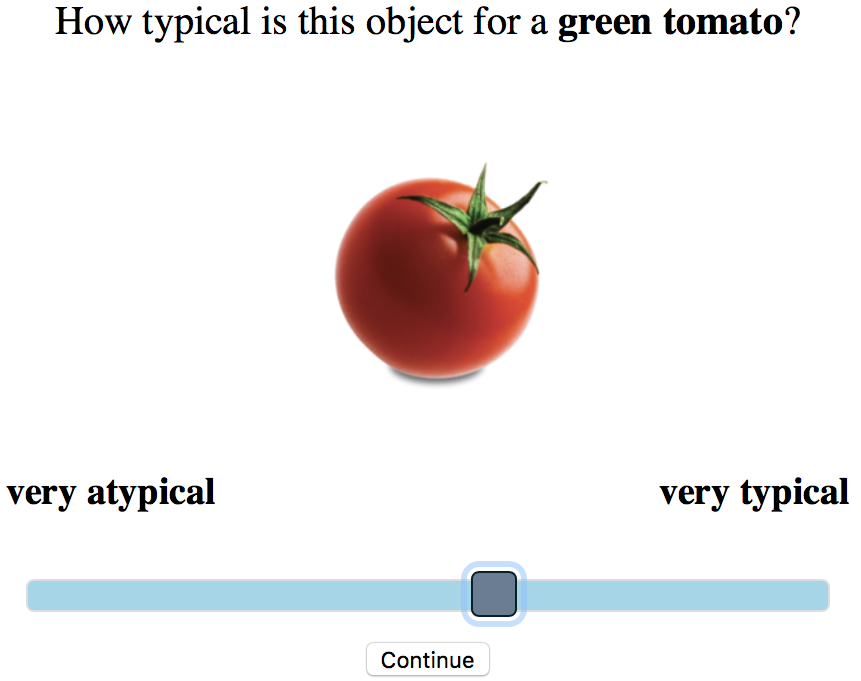
\includegraphics[width=.5\textwidth]{pics/typ_norm_full_2}
	\caption{A typical trial in the `Adj Noun' typicality norming study.
	}
	\label{fig:typicalitynorming}
\end{figure}


\begin{table*}
\caption{Overview of typicality norming studies. \jd{update this to reflect updated participant number for holistic norms}}
\begin{tabular}{l l l l l l l}
\toprule
Utterances & Example & Images & Participants & Trials & Items & Excluded\\
\midrule
Adj Noun & \emph{yellow banana} & object & 66 & 110 & 484 & 4\\ 
Noun & \emph{banana} & object & 75 & 90 & 198 & 1\\
Adj & \emph{yellow} & color patch & 75 & 90 & 176 & None\\
\bottomrule
\end{tabular}
\label{tab:normingoverview}
\end{table*}

Slider values were coded as falling between 0 (`very atypical') and 1 (`very typical'). For each utterance-object combination we computed mean typicality ratings. For example, mean typicalities for the banana items are shown in \tableref{tab:bananatypicalities}.

\begin{table}
\caption{Mean typicalities for banana items. Combinations where a deterministic semantics would return TRUE are marked in boldface.}
\begin{tabular}{r r r r r}
\toprule
%Utterance & Item & Typicality\\
 & \multicolumn{3}{c}{Banana items} & Other \\
 Utterance & yellow & brown  & blue & \\ 
 \midrule
\emph{banana} & \textbf{.98} & \textbf{.66} & \textbf{.42} & .05  \\
 \midrule
\emph{yellow banana} & \textbf{.98} & .33 & .17 & .05 \\
\emph{brown banana} & .28 & \textbf{.90} & .18 & .04\\
\emph{blue banana} & .20 & .18 & \textbf{.91} & .06\\
\midrule
\emph{yellow} & \textbf{.77} & .05 & .06 & .09\\
\emph{brown} & .11 & \textbf{.87} & .01 & .12\\
\emph{blue} & .06 & .06 & \textbf{.92} & .07\\
\bottomrule
\end{tabular}
\label{tab:bananatypicalities}
\end{table}


\jd{change the following discussion; replace with previous prose you wrote on this for this section?}
The way we elicited typicalities differs somewhat from the approach taken in previous work \cite<e.g.>{Westerbeek2015}, where participants are typically asked ``How typical is this color for this object?'' We deviated from this because for the purpose of testing the model (see below), what is required is the degree of applicability of an utterance to an object, rather than the degree to which an object's color is representative of that object. We expect, however, that the simple noun-object typicalities will yield very similar results as the Westerbeek question because the employed objects are color-diagnostic -- asking whether an blue or a yellow banana is a typical \emph{banana} is similar to asking whether or not the bananas' most salient property -- their color -- is typical. 

\subsection{Results and discussion}

Proportions of type-only (\emph{banana}), color-and-type (\emph{yellow banana}), color-only (\emph{yellow}), and other (\emph{funky carrot}) are shown in \figref{fig:proportions}. Visually inspecting just the explicitly marked \emph{yellow banana}, \emph{brown banana}, and \emph{blue banana} cases suggests a clear typicality effect in the overinformative conditions as well as a smaller typicality effect in the informative conditions. 

\begin{figure}[bt]
\centering
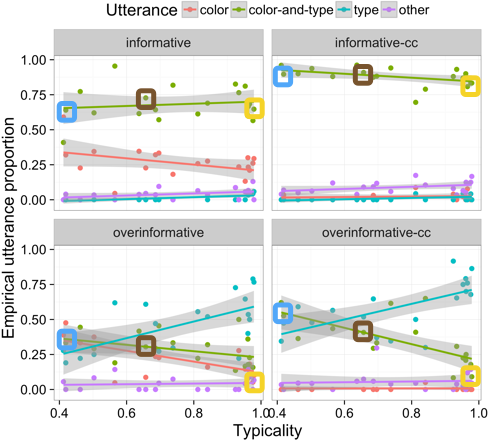
\includegraphics[width=.8\textwidth]{pics/results1.png}
\caption{For each target, proportion of color-only (\emph{yellow}), type-only (\emph{banana}), color-and-type (\emph{yellow banana}), and other (\emph{funky carrot}) utterances as a function of mean object typicality for the type-only utterance, across conditions. \emph{\textsc{color} banana} cases are circled in their respective color.}
\label{fig:proportions}
\end{figure}

The following questions are of interest. First, do we replicate the previously documented typicality effect on redundant color mention beyond the one-item visual inspection? Second, do we observe typicality effects even when color is informative (i.e., technically necessary for establishing unique reference)? Third, are speakers sensitive to the presence of color competitors in their use of color or are typicality effects immune to the nature of the distractor items?

To address these questions we conducted a mixed effects logistic regression predicting color use from fixed effects of typicality, informativeness, and color competitor presence. We used the typicality norms obtained in the noun-object typicality elicitation study reported above as the continuous typicality predictor. Informativeness was coded as a binary variable (color \emph{informative} vs.~color overinformative) as was color competitor presence (absent vs.~present). All predictors were centered before entering the analysis. The model included by-speaker and by-item random intercepts, which was the maximal random effects structure that allowed the model to converge.

There was a main effect of typicality, such that the more typical an object was for the noun, the lower the log odds of color mention ($\beta$ = -3.19, $SE$ = 0.36, $p <$ .0001), replicating previously documented typicality effects. Model comparison revealed that including interaction terms was not justified by the data, suggesting that speakers produce more typical colors less often even when the color is in principle necessary for establishing reference (i.e., in the informative conditions). There was also a main effect of informativeness, such that color mention was more likely when it was informative than when it was overinformative   ($\beta$ = 3.32, $SE$ = 0.16, $p <$ .0001). Finally, there was a main effect of color competitor presence, such that color mention was less likely when a color competitor was present  ($\beta$ = -0.66, $SE$ = 0.13, $p <$ .0001). This suggests that speakers are indeed sensitive to the contextual utility of color -- color typicality alone does not capture the full set of facts about color mention.

\jd{update all the following prose -- change the first section into a footnote to demonstrate that we also have typicality effects in the dataset from exp 1}
In this section we have reported the replication of previously documented typicality effects on color mention as well as a novel demonstration of typicality effects even when color is informative. We have also shown that color mention is sensitive not only to typicality, but also to the  nature of the distractors -- when there is another distractor of the same color as the target, color is dispreferred compared to when there is not. 
%What this suggests is that choosing to include a color modifier in a referring expression is not just a function of one factor. While it is clear that 
Thus far we have only been concerned with analyzing the use of color, i.e., we collapsed \textsc{color} and \textsc{color-and-type} utterances into one category. However, our goal is to formulate a cognitive model that captures the production of referring expressions more generally. To this we turn next.

%%% CHECK UP TO HERE -- NEXT IS OLD PROSE

To assess whether we replicate the color typicality effects previously reported in the literature \cite{sedivy2003a, Westerbeek2015, rubiofernandez2016}, we elicited color typicality norms for each of our items and then included typicality as an additional predictor of redundant adjective use in the regression analysis reported previously. 
%See \appref{app:typicalityexperiment} for a detailed description of the methodology and materials.

\subsubsection{Methods}

\paragraph{Participants}

We recruited 60 participants over Amazon's Mechanical Turk who were each paid \$0.25 for their participation.

\paragraph{Procedure and materials}

On each trial, participants saw one of the big versions of the items used in Exp.~1 and were asked to answer the question ``How typical is this for an \emph{X}?'' on a continuous slider with endpoints labeled ``very atypical'' to ``very typical.'' \emph{X} was a referring expression consisting of either only the correct noun (e.g., \emph{stapler}) or the noun modified by the correct color (e.g., \emph{red stapler}). \figref{fig:modifiertypstimulus} shows an example of a modified trial.

Each participant saw each of the 36 objects once. An object was randomly displayed in one of the two colors it occurred with in Exp.~1 and was randomly displayed with either the correct modified utterance or the correct unmodified utterance, in order to obtain roughly equal numbers of object-utterance combinations.

\begin{figure}
\centering
\includegraphics[width=.5\textwidth]{pics/redstapler.png}
\caption{A modified example trial from the typicality elicitation experiment.}
\label{fig:modifiertypstimulus}
\end{figure}

Importantly, we only elicited typicality norms for unmodified utterances and utterances with color modifiers, but not utterances with size modifiers. This was because it is virtually impossible to obtain size typicality norms for objects presented in isolation, due to the inherently relational nature of size adjectives. Consequently, we only test for the effect of typicality on \emph{size-sufficient} trials.


\subsubsection{Results and discussion}

We coded the slider endpoints as 0 (``very atypical'') and 1 (``very typical''), essentially treating each response as a typicality value between 0 and 1. For each combination of object, color, and utterance (modified/unmodified), we computed that item's mean. Mean typicalities were generally lower for unmodified than for modified utterances: mean typicality for unmodified utterances was .67 (sd=.17, mode=.76) and for modified utterances .75 (sd=.12, mode=.81). This can also be seen on the left in \figref{fig:typicalitydists}. Note that, as expected given how the stimuli were constructed, typicality was generally skewed towards the high end, even for unmodified utterances. This means that there was not much variation in  the difference in typicality between modified and unmodified utterances. We will refer to this difference as \emph{typicality gain}, reflecting the overall gain in typicality via color modification over the unmodified baseline. As can be seen on the right in \figref{fig:typicalitydists}, in most cases typicality gain was close to zero.

\begin{figure}
\centering
\includegraphics[width=.9\textwidth]{pics/typicality-dists}
\caption{Typicality densities for modified and unmodified utterances (left) and histogram of typicality gains (differences between modified and unmodified typicalities, right).}
\label{fig:typicalitydists}
\end{figure}

This makes the typicality analysis difficult: if typicality gain is close to zero for most cases (and, taking into account confidence intervals, effectively zero), it is hard to evaluate the effect of typicality on redundant adjective use. In order to maximize power, we therefore conducted the analysis only on those items for which for at least one color the confidence intervals for the modified and unmodified utterances did not overlap. There were only four such cases: \emph{(pink) golfball}, \emph{(pink) wedding cake}, \emph{(green) chair}, and \emph{(red) stapler}, for a total of 231 data points.

Predictions differ for size-sufficient and color-sufficient trials. Given the typicality effects reported in the literature and the predictions of non-deterministic RSA, we expect greater redundant color use on size-sufficient trials with \emph{increasing} typicality gain. The predictions for redundant size use on color-sufficient trials are unclear from the previous literature. Non-deterministic RSA, however,  predicts greater redundant size use with \emph{decreasing} typicality gain: small color typicality gains reflect the relatively low out-of-context utility of color. In these cases, it may be useful to redundantly use a size modifier even if that modifier is noisy. If borne out, these predictions should surface in an interaction between sufficient property and typicality gain. Visual inspection of the empirical proportions of redundant adjective use in \figref{fig:maxtypicalitydiff} suggests that this pattern is indeed borne out.

\begin{figure}
\centering
\includegraphics[width=.9\textwidth]{pics/maxtypicalitydiff}
\caption{Utterance probability for four items as a function of difference in typicality between modified and unmodified utterance (x-axis) and sufficient dimension (columns). }
\label{fig:maxtypicalitydiff}
\end{figure}

In order to investigate the effect of typicality gain on redundant adjective use, we conducted a mixed effects logistic regression analysis predicting redundant over minimal adjective use from fixed effects of scene variation, sufficient dimension, the interaction of scene variation and sufficient property, and the interaction of typicality gain and sufficient property. This is the same model as reported in \sectionref{sec:modelempiricalresults}, with the only difference that the interaction between sufficient property and typicality gain was added. All predictors were centered before entering the analysis. The model contained the maximal random effects structure that allowed it to converge: by-participant and by-item (where item was a color-object combination) random intercepts. 

The model summary is shown in \tableref{tab:colortypicalityresults}. We replicate the effects of sufficient property and scene variation observed earlier on this smaller dataset. Crucially, we observe a significant interaction between sufficient property and typicality gain.\footnote{Conducting the same analysis on the entire dataset (i.e., using all of the noisy typicality estimates, replicated the scene variation and sufficient property effects. The interaction of typicality gain and sufficient property went in the same direction numerically, but failed to reach significance ($\beta = 1.52$, $SE = 1.45$, $p < .29$).} Simple effects analysis reveals that this interaction is due to a positive effect of typicality gain on redundant adjective use in the size-sufficient condition ($\beta = 4.47$, $SE = 1.65$, $p < .007$) but a negative effect of typicality gain on redundant adjective use in the color-sufficient condition  ($\beta = -5.77$, $SE = 2.49$, $p < .03$). 

\begin{table}[!tbp]
\caption{Model coefficients, standard errors, and p-values. Significant p-values are bolded.}
\begin{center}
\begin{tabular}{lrrl}
\toprule
\multicolumn{1}{l}{}&\multicolumn{1}{c}{Coef $\beta$}&\multicolumn{1}{c}{SE($\beta$)}&\multicolumn{1}{c}{$p$}\tabularnewline
\midrule
Intercept&$-1.85$&$0.34$&\textbf{\textless .0001}\tabularnewline
Scene variation&$ 4.29$&$1.16$&\textbf{\textless .001}\tabularnewline
Sufficient property&$ 2.72$&$0.60$&\textbf{\textless .0001}\tabularnewline
Scene variation : Sufficient property&$ 0.88$&$2.12$&\textless 0.68\tabularnewline
Sufficient property : Typicality gain&$ 9.43$&$2.68$&\textbf{\textless .001}\tabularnewline
\bottomrule
\end{tabular}\end{center}
\label{tab:colortypicalityresults}
\end{table}

An important point is of note: the typicality elicitation procedure we employed here is somewhat different from that employed by \citeA{Westerbeek2015}, who asked their participants ``How typical is this color for this object?'' We did this for conceptual reasons: the values that go into the semantics of the RSA model are most easily conceptualized as the typicality of an object as an instance of an utterance. While the typicality of a feature for an object type no doubt plays into how good of an instance of the utterance the object is, deriving our typicalities from the  statistical properties of the subjective distributions of features over objects is beyond the scope of this paper. However, in a separate experiment we did ask participants the Westerbeek question. The correlation between mean typicality ratings from the Westerbeek version and the unmodified ``How typical is this for \emph{X}'' version was .75. The correlation between the Westerbeek version and the modified version was .64. The correlation between the Westerbeek version and typicality gain was -.52.

For comparison, including typicality means obtained via the Westerbeek question as a predictor instead of typicality gain on the four high-powered items replicated the significant interaction between typicality and sufficient property ($\beta = -6.77$, $SE = 1.88$, $p < .0003$). Simple effects analysis revealed that the interaction is again due to a difference in slope in the two sufficient property conditions: in the size-sufficient condition, color is less likely to be mentioned with increasing color typicality   ($\beta = -3.66$, $SE = 1.18$, $p < .002$), whereas in the color-sufficient condition, size is more likely to be mentioned with increasing color typicality ($\beta = 3.09$, $SE = 1.45$, $p < .04$).\footnote{Again, conducting this analysis on the entire dataset yielded only a marginal interaction of sufficient property and color typicality in the right direction ($\beta = -1.10$, $SE = .64$, $p < .09$).}

We thus overall find moderate evidence for typicality effects in our dataset. Typicality effects are strong for those items that clearly display typicality differences between the modified and unmodified utterance, but much weaker for the remaining items. That the evidence for typicality effects is relatively scarce is no surprise: the stimuli were specifically designed to minimize effects of typicality. However, the fact that both ways of quantifying typicality predicted redundant adjective use in the expected direction suggests that with more power or with stimuli that exhibit greater typicality variation, these effects may show up more clearly.

In the next section we evaluate whether the fit of non-deterministic RSA to the data is improved by using the empirically elicited typicalities as the values in the non-deterministic semantics.

\subsection{Model evaluation: color typicality}
\label{sec:modelevalcolortypicality}

\jd{complete overhaul of the model section after update}

%\jd{insert actual numbers below! figure out what's going wrong in the bda that the returned color fidelities are lower than the returned size fidelities}

In order to evaluate the effect of utterance-object level typicality we proceed in two steps: first, we present the results of performing Bayesian data analysis in the same way as reported in \sectionref{sec:modifiermodeleval}, with the only difference that instead of fixed utterance type level fidelities we include the more fine-grained fidelity values corresponding to the typicality norms. We will focus more closely on the four items shown in \figref{fig:maxtypicalitydiff} in order to demonstrate the effect of including typicality in the model \red{once you know, actually put a summary sentence here instead of "in order to see how the model bla"}. In a second step we then address the pressing question of whether more fine-grained typicalities add any predictive value. 

\subsubsection{Model evaluation: empirical typicalities}

In order to generate model predictions and infer likely parameter values for the dataset reported above,  we repeated the same Bayesian data analysis procedure as described above, with one difference: instead of using the utterance-type level fidelities we fed the model the empirically elicited typicality norms. This was slightly less trivial than it sounds for two reasons. First, we only elicited typicality norms for object-utterance pairs for which the utterance was either just the simple object category noun (e.g., \emph{chair}) or the color-modified noun (e.g., \emph{green chair}); that is, we did not elicit size typicality norms (for reasons described in the previous section). Second, we did not elicit typicality norms for utterance-object pairs where the object would not be in the deterministic semantics' extension (e.g., \emph{green chair} used to refer to a red chair). In order to fill in the typicality gaps, so to speak, we assigned fidelity values to utterances as follows: object-utterance pairs where the object is in the extension of the utterance were assigned the empirically elicited typicality for that pair (e.g., \emph{chair} typicality for any chair, \emph{red chair} typicality for red chairs, see \tableref{tab:empiricalcolorfidelities}). If the object was not in the utterance extension, it received a fidelity of $1 - f_{c}$, where $f_c$ is an utterance type level fidelity parameter for color (as in the basic non-deterministic model reported above). For objects in the utterance extension where the utterance additionally contained a size modifier, the empirical fidelity was multiplied by an utterance type level size fidelity $f_{s}$. See \tableref{tab:empiricalcolorfidelities} for an overview of fidelity values for one item (red/green chair). 


\begin{table}
\centering
\caption{\jd{get rid of this!} Fidelity values (rescaled) for one example item (chair) that occurred in two colors (red, green). Rows indicate different utterances, columns indicate different objects. See \tableref{tab:empiricalscaledunscaledtyps} for the raw and rescaled empirical typicality values for the red/green chair item.\jd{redo this whole table now that you're doing the right thing and summing. weird thing: do we want a size+type utterance (e.g.) to have more utility than just the type utterance if size modifier is "wrong"? because that's what's currently happening. ie, adding any additional modifier is adding utility}}
\begin{tabular}{l l l l l}
\toprule
Utterance & small red chair & small green chair & big red chair & big green chair\\
\midrule
\emph{chair} & .83 & .67 & .83 & .67 \\
\emph{red chair} & .84 & $.67+(1 - f_{\textrm{c}}$) & .84 & $.67 + (1 - f_{\textrm{c}}$) \\
\emph{green chair} & .83 + ($1 - f_{\textrm{c}}$) & .85 & .83 + ($1 - f_{\textrm{c}}$) & .85 \\
\emph{small chair} & .83 + $f_{\textrm{s}}$ &  .67 + $f_{\textrm{s}}$ & .83 + $(1 - f_{\textrm{s}})$ & .67 + $(1 - f_{\textrm{s}})$ \\
\emph{big chair} & .83 + $(1 - f_{\textrm{s}})$ & .67 + $(1 - f_{\textrm{s}})$ &  .83 + $f_{\textrm{s}}$ &  .67 + $f_{\textrm{s}}$ \\
\emph{small red chair} &  .84 + $f_{\textrm{s}}$ & .67 + $f_{\textrm{s}} + (1 - f_{\textrm{c}})$ & .84 + $(1 - f_{\textrm{s}})$ & .67 + $(1-f_{\textrm{s}}) + (1-f_{\textrm{c}})$ \\
\emph{big red chair} &  .84 + $(1-f_{\textrm{s}})$ & .67 + $(1-f_{\textrm{s}}) + (1-f_{\textrm{c}})$ &  .84 + $f_{\textrm{s}}$ & .67 + $f_{\textrm{s}} + (1-f_{\textrm{c}})$ \\
\emph{small green chair} & .83 + $f_{\textrm{s}} + (1-f_{\textrm{c}})$ & $f_{\textrm{s}} \jd{conthere}\cdot .85 $ & $(1-f_{\textrm{s}}) \cdot (1-f_{\textrm{c}})$ & $(1-f_{\textrm{s}}) \cdot .85$ \\
\emph{big green chair} & $(1-f_{\textrm{s}}) \cdot (1-f_{\textrm{c}})$ & .$(1-f_{\textrm{s}}) \cdot .85$ & $f_{\textrm{s}} \cdot (1-f_{\textrm{c}})$ & $f_{\textrm{s}} \cdot .85$ \\
\bottomrule
\end{tabular}
\label{tab:empiricalcolorfidelities}
\end{table}

One final point of note: empirically elicited typicality values were rescaled to range from 0.5 to 1 (instead of from 0 to 1). This was done because a fidelity value of .5, when there are only two potential feature values (e.g., two colors in the scene, red and green), leads to a random choice between green and red items; that is, the modifier contains no information. When the fidelity value is below .5 in these two-feature value scenarios, the modifier contextually acquires the meaning of the other feature dimension, e.g., \emph{green} is more likely to pick out red than green objects. The typicality values we elicited were not degree of membership values (which is what the model expects). Rather, they are more comparable to distance from prototype values \cite<see>[for a discussion of the difference]{kamp1995}. By rescaling the empirical typicality values to fall above .5, we guaranteed that the utterance would have at least an above chance of meaning what it would mean under a deterministic semantics. \tableref{tab:empiricalscaledunscaledtyps} exemplifies the effect of rescaling the raw typicality values for the red/green chair item.

\begin{table}
\centering
\caption{Raw and rescaled typicalities for the red and green chair items. \emph{NA} values indicate cases where typicality for that utterance-object combination was not elicited (e.g., \emph{green chair} applied to a red chair).}
\begin{tabular}{l l l l l}
\toprule
& \multicolumn{2}{c}{Raw} & \multicolumn{2}{c}{Rescaled}\\
Utterance & red chair & green chair & red chair & green chair\\
\midrule
\emph{chair} & .68 & .41 & .83 & .67\\
\emph{red chair} & .69 & NA & .84 & NA\\
\emph{green chair} & NA & .70  & NA & .85\\
\bottomrule
\end{tabular}
\label{tab:empiricalscaledunscaledtyps}
\end{table}

\paragraph{Results} Including typicality  yielded similar item-wise model-data correlations as the basic model \red{XXX}. Posteriors over parameters are shown in \figref{fig:typicalityparamposteriors}. \red{Discuss similarities/diffs to basic model.} 

\begin{figure}
\label{fig:typicalityparamposteriors}
%\includegraphics{bla}
\caption{\red{Posterior distribution over model parameters. Maximum a posteriori (MAP)  $f_{\textrm{s}}$ = 0.79, 95\% highest density interval (HDI) = [0.76,0.80]; MAP $f_{\textrm{c}}$ = 0.88, HDI = [0.86,0.91]; MAP $c_{\textrm{size}}$ = .08, HDI = [0, 1.5]; MAP $c_{\textrm{color}}$ = 0.07, HDI = [0,0.9]; MAP $\beta_c$ = 0.04, HDI = [0,1.6]; MAP $\alpha$ = 34.0, HDI = [30.8,36.5]}}
\end{figure}

Posterior predictives for the cases with greatest typicality gain -- \emph{chair}, \emph{golfball}, \emph{weddingcake}, and \emph{stapler} -- are shown in \figref{fig:ppmaxtypdiff} alongside the posterior predictives from the basic model (with utterance type level fidelities). In the basic non-deterministic model, probability of redundant utterances is similar for items of different colors. In the model that includes empirically elicited typicalities, the probability of redundant utterances is greater where typicality gain is greater; that is, for cases where the unmodified utterance has low typicality and the modified utterance high typicality, analogous to the \emph{blue banana} case.

\subsubsection{Model evaluation: interpolation analysis}

Because the correlations between model-predicted utterance probability posterior predictives and empirical proportions are very similar across the basic and empirical typicality model, the question arises whether utterance-level typicalities add any predictive value whatsoever. In order to address this question we present a second BDA analysis in which we introduce an additional parameter in the model that functions as a weight on fidelity type: if the weight is 0, only the utterance-type level fidelities are used; if the weight is 1 only the empirical typicalities are used. Therefore, if the BDA returns posterior values for fidelity type weight greater than 0, empirical typicalities are justified.

\paragraph{Results} Posteriors over parameters are shown in \figref{fig:interpolposteriors}. \red{insert figure} The MAP estimate for fidelity type weight is \red{XXX (HDI = [X,X])}, suggesting that utterance-level typicality adds predictive value.

\begin{figure}
\label{fig:interpolposteriors}
%\includegraphics{bla}
\caption{\red{Posterior distribution over model parameters. Maximum a posteriori (MAP)  $f_{\textrm{s}}$ = 0.79, 95\% highest density interval (HDI) = [0.76,0.80]; MAP $f_{\textrm{c}}$ = 0.88, HDI = [0.86,0.91]; MAP $c_{\textrm{size}}$ = .08, HDI = [0, 1.5]; MAP $c_{\textrm{color}}$ = 0.07, HDI = [0,0.9]; MAP $\beta_c$ = 0.04, HDI = [0,1.6]; MAP $\alpha$ = 34.0, HDI = [30.8,36.5]}}
\end{figure}

\subsection{Discussion}

\red{main points: a) that non-deterministic RSA with utterance-level typicalities as fidelity values captures the color typicality effects reported in the literature qualitatively (yellow/blue banana); b) that even in our dataset, where items were designed to not exhibit great typicality effects, we find evidence of typicality effects on utterance probability, replicating previous studies; and c) BDA shows that including empirically elicited typicality norms in the model adds predictive value. This suggests that speakers are tracking typicality at a very fine-grained level}.

\jd{This is all well and good, but to what extent is non-deterministic RSA just a model of modifier choice in modified referring expressions? Put differently, does non-deterministic RSA provide a good account of content selection in referring expressions more generally? To answer this question we move beyond modified referring expressions and turn to simple nominal referring expressions.}

In the next section we turn to extending non-deterministic RSA beyond the choice of modifier.


%We can now ask whether taking into account this more fine-grained notion of non-deterministic semantics plays a role in the dataset collected in Exp.~1. 
%%\sectionref{sec:exp1-scenevar}. 
%A note upfront: the stimuli for Exp.~1 were specifically designed to be realistic objects; that is, very low typicality values or even a large degree of variation in typicality would be surprising. Nevertheless, it is plausible that typicality differences exist. If they do, there are two interesting questions to ask: first, do we replicate the typicality effects reported in the literature -- that is, are less typical objects more likely to lead to redundant adjective use than more typical objects? Second, does including empirically elicited typicality values at the object-utterance level further improve the quality of the RSA model? We address the first question in \sectionref{sec:modifiertypicalityeffects} and the second question in \sectionref{sec:modelevalcolortypicality}.

%\subsection{Experiment 1a: Typicality effects in Exp.~1}
%\label{sec:modifiertypicalityeffects}
%
%To assess whether we replicate the color typicality effects previously reported in the literature \cite{sedivy2003a, Westerbeek2015, rubiofernandez2016}, we elicited color typicality norms for each of our items and then included typicality as an additional predictor of redundant adjective use in the regression analysis reported previously. 
%%See \appref{app:typicalityexperiment} for a detailed description of the methodology and materials.
%
%\subsubsection{Methods}
%
%\paragraph{Participants}
%
%We recruited 60 participants over Amazon's Mechanical Turk who were each paid \$0.25 for their participation.
%
%\paragraph{Procedure and materials}
%
%On each trial, participants saw one of the big versions of the items used in Exp.~1 and were asked to answer the question ``How typical is this for an \emph{X}?'' on a continuous slider with endpoints labeled ``very atypical'' to ``very typical.'' \emph{X} was a referring expression consisting of either only the correct noun (e.g., \emph{stapler}) or the noun modified by the correct color (e.g., \emph{red stapler}). \figref{fig:modifiertypstimulus} shows an example of a modified trial.
%
%Each participant saw each of the 36 objects once. An object was randomly displayed in one of the two colors it occurred with in Exp.~1 and was randomly displayed with either the correct modified utterance or the correct unmodified utterance, in order to obtain roughly equal numbers of object-utterance combinations.
%
%\begin{figure}
%\centering
%\includegraphics[width=.5\textwidth]{pics/redstapler.png}
%\caption{A modified example trial from the typicality elicitation experiment.}
%\label{fig:modifiertypstimulus}
%\end{figure}
%
%Importantly, we only elicited typicality norms for unmodified utterances and utterances with color modifiers, but not utterances with size modifiers. This was because it is virtually impossible to obtain size typicality norms for objects presented in isolation, due to the inherently relational nature of size adjectives. Consequently, we only test for the effect of typicality on \emph{size-sufficient} trials.
%
%
%\subsubsection{Results and discussion}
%
%We coded the slider endpoints as 0 (``very atypical'') and 1 (``very typical''), essentially treating each response as a typicality value between 0 and 1. For each combination of object, color, and utterance (modified/unmodified), we computed that item's mean. Mean typicalities were generally lower for unmodified than for modified utterances: mean typicality for unmodified utterances was .67 (sd=.17, mode=.76) and for modified utterances .75 (sd=.12, mode=.81). This can also be seen on the left in \figref{fig:typicalitydists}. Note that, as expected given how the stimuli were constructed, typicality was generally skewed towards the high end, even for unmodified utterances. This means that there was not much variation in  the difference in typicality between modified and unmodified utterances. We will refer to this difference as \emph{typicality gain}, reflecting the overall gain in typicality via color modification over the unmodified baseline. As can be seen on the right in \figref{fig:typicalitydists}, in most cases typicality gain was close to zero.
%
%\begin{figure}
%\centering
%\includegraphics[width=.9\textwidth]{pics/typicality-dists}
%\caption{Typicality densities for modified and unmodified utterances (left) and histogram of typicality gains (differences between modified and unmodified typicalities, right).}
%\label{fig:typicalitydists}
%\end{figure}
%
%This makes the typicality analysis difficult: if typicality gain is close to zero for most cases (and, taking into account confidence intervals, effectively zero), it is hard to evaluate the effect of typicality on redundant adjective use. In order to maximize power, we therefore conducted the analysis only on those items for which for at least one color the confidence intervals for the modified and unmodified utterances did not overlap. There were only four such cases: \emph{(pink) golfball}, \emph{(pink) wedding cake}, \emph{(green) chair}, and \emph{(red) stapler}, for a total of 231 data points.
%
%Predictions differ for size-sufficient and color-sufficient trials. Given the typicality effects reported in the literature and the predictions of non-deterministic RSA, we expect greater redundant color use on size-sufficient trials with \emph{increasing} typicality gain. The predictions for redundant size use on color-sufficient trials are unclear from the previous literature. Non-deterministic RSA, however,  predicts greater redundant size use with \emph{decreasing} typicality gain: small color typicality gains reflect the relatively low out-of-context utility of color. In these cases, it may be useful to redundantly use a size modifier even if that modifier is noisy. If borne out, these predictions should surface in an interaction between sufficient property and typicality gain. Visual inspection of the empirical proportions of redundant adjective use in \figref{fig:maxtypicalitydiff} suggests that this pattern is indeed borne out.
%
%\begin{figure}
%\centering
%\includegraphics[width=.9\textwidth]{pics/maxtypicalitydiff}
%\caption{Utterance probability for four items as a function of difference in typicality between modified and unmodified utterance (x-axis) and sufficient dimension (columns). }
%\label{fig:maxtypicalitydiff}
%\end{figure}
%
%In order to investigate the effect of typicality gain on redundant adjective use, we conducted a mixed effects logistic regression analysis predicting redundant over minimal adjective use from fixed effects of scene variation, sufficient dimension, the interaction of scene variation and sufficient property, and the interaction of typicality gain and sufficient property. This is the same model as reported in \sectionref{sec:modelempiricalresults}, with the only difference that the interaction between sufficient property and typicality gain was added. All predictors were centered before entering the analysis. The model contained the maximal random effects structure that allowed it to converge: by-participant and by-item (where item was a color-object combination) random intercepts. 
%
%The model summary is shown in \tableref{tab:colortypicalityresults}. We replicate the effects of sufficient property and scene variation observed earlier on this smaller dataset. Crucially, we observe a significant interaction between sufficient property and typicality gain.\footnote{Conducting the same analysis on the entire dataset (i.e., using all of the noisy typicality estimates, replicated the scene variation and sufficient property effects. The interaction of typicality gain and sufficient property went in the same direction numerically, but failed to reach significance ($\beta = 1.52$, $SE = 1.45$, $p < .29$).} Simple effects analysis reveals that this interaction is due to a positive effect of typicality gain on redundant adjective use in the size-sufficient condition ($\beta = 4.47$, $SE = 1.65$, $p < .007$) but a negative effect of typicality gain on redundant adjective use in the color-sufficient condition  ($\beta = -5.77$, $SE = 2.49$, $p < .03$). 
%
%\begin{table}[!tbp]
%\caption{Model coefficients, standard errors, and p-values. Significant p-values are bolded.}
%\begin{center}
%\begin{tabular}{lrrl}
%\toprule
%\multicolumn{1}{l}{}&\multicolumn{1}{c}{Coef $\beta$}&\multicolumn{1}{c}{SE($\beta$)}&\multicolumn{1}{c}{$p$}\tabularnewline
%\midrule
%Intercept&$-1.85$&$0.34$&\textbf{\textless .0001}\tabularnewline
%Scene variation&$ 4.29$&$1.16$&\textbf{\textless .001}\tabularnewline
%Sufficient property&$ 2.72$&$0.60$&\textbf{\textless .0001}\tabularnewline
%Scene variation : Sufficient property&$ 0.88$&$2.12$&\textless 0.68\tabularnewline
%Sufficient property : Typicality gain&$ 9.43$&$2.68$&\textbf{\textless .001}\tabularnewline
%\bottomrule
%\end{tabular}\end{center}
%\label{tab:colortypicalityresults}
%\end{table}
%
%An important point is of note: the typicality elicitation procedure we employed here is somewhat different from that employed by \citeA{Westerbeek2015}, who asked their participants ``How typical is this color for this object?'' We did this for conceptual reasons: the values that go into the semantics of the RSA model are most easily conceptualized as the typicality of an object as an instance of an utterance. While the typicality of a feature for an object type no doubt plays into how good of an instance of the utterance the object is, deriving our typicalities from the  statistical properties of the subjective distributions of features over objects is beyond the scope of this paper. However, in a separate experiment we did ask participants the Westerbeek question. The correlation between mean typicality ratings from the Westerbeek version and the unmodified ``How typical is this for \emph{X}'' version was .75. The correlation between the Westerbeek version and the modified version was .64. The correlation between the Westerbeek version and typicality gain was -.52.
%
%For comparison, including typicality means obtained via the Westerbeek question as a predictor instead of typicality gain on the four high-powered items replicated the significant interaction between typicality and sufficient property ($\beta = -6.77$, $SE = 1.88$, $p < .0003$). Simple effects analysis revealed that the interaction is again due to a difference in slope in the two sufficient property conditions: in the size-sufficient condition, color is less likely to be mentioned with increasing color typicality   ($\beta = -3.66$, $SE = 1.18$, $p < .002$), whereas in the color-sufficient condition, size is more likely to be mentioned with increasing color typicality ($\beta = 3.09$, $SE = 1.45$, $p < .04$).\footnote{Again, conducting this analysis on the entire dataset yielded only a marginal interaction of sufficient property and color typicality in the right direction ($\beta = -1.10$, $SE = .64$, $p < .09$).}
%
%We thus overall find moderate evidence for typicality effects in our dataset. Typicality effects are strong for those items that clearly display typicality differences between the modified and unmodified utterance, but much weaker for the remaining items. That the evidence for typicality effects is relatively scarce is no surprise: the stimuli were specifically designed to minimize effects of typicality. However, the fact that both ways of quantifying typicality predicted redundant adjective use in the expected direction suggests that with more power or with stimuli that exhibit greater typicality variation, these effects may show up more clearly.
%
%In the next section we evaluate whether the fit of non-deterministic RSA to the data is improved by using the empirically elicited typicalities as the values in the non-deterministic semantics.
%
%\subsection{Model evaluation: color typicality}
%\label{sec:modelevalcolortypicality}
%
%\jd{insert actual numbers below! figure out what's going wrong in the bda that the returned color fidelities are lower than the returned size fidelities}
%
%In order to evaluate the effect of utterance-object level typicality we proceed in two steps: first, we present the results of performing Bayesian data analysis in the same way as reported in \sectionref{sec:modifiermodeleval}, with the only difference that instead of fixed utterance type level fidelities we include the more fine-grained fidelity values corresponding to the typicality norms. We will focus more closely on the four items shown in \figref{fig:maxtypicalitydiff} in order to demonstrate the effect of including typicality in the model \red{once you know, actually put a summary sentence here instead of "in order to see how the model bla"}. In a second step we then address the pressing question of whether more fine-grained typicalities add any predictive value. 
%
%\subsubsection{Model evaluation: empirical typicalities}
%
%In order to generate model predictions and infer likely parameter values for the dataset reported above,  we repeated the same Bayesian data analysis procedure as described above, with one difference: instead of using the utterance-type level fidelities we fed the model the empirically elicited typicality norms. This was slightly less trivial than it sounds for two reasons. First, we only elicited typicality norms for object-utterance pairs for which the utterance was either just the simple object category noun (e.g., \emph{chair}) or the color-modified noun (e.g., \emph{green chair}); that is, we did not elicit size typicality norms (for reasons described in the previous section). Second, we did not elicit typicality norms for utterance-object pairs where the object would not be in the deterministic semantics' extension (e.g., \emph{green chair} used to refer to a red chair). In order to fill in the typicality gaps, so to speak, we assigned fidelity values to utterances as follows: object-utterance pairs where the object is in the extension of the utterance were assigned the empirically elicited typicality for that pair (e.g., \emph{chair} typicality for any chair, \emph{red chair} typicality for red chairs, see \tableref{tab:empiricalcolorfidelities}). If the object was not in the utterance extension, it received a fidelity of $1 - f_{c}$, where $f_c$ is an utterance type level fidelity parameter for color (as in the basic non-deterministic model reported above). For objects in the utterance extension where the utterance additionally contained a size modifier, the empirical fidelity was multiplied by an utterance type level size fidelity $f_{s}$. See \tableref{tab:empiricalcolorfidelities} for an overview of fidelity values for one item (red/green chair). 
%
%
%\begin{table}
%\centering
%\caption{Fidelity values (rescaled) for one example item (chair) that occurred in two colors (red, green). Rows indicate different utterances, columns indicate different objects. See \tableref{tab:empiricalscaledunscaledtyps} for the raw and rescaled empirical typicality values for the red/green chair item.\jd{redo this whole table now that you're doing the right thing and summing. weird thing: do we want a size+type utterance (e.g.) to have more utility than just the type utterance if size modifier is "wrong"? because that's what's currently happening. ie, adding any additional modifier is adding utility}}
%\begin{tabular}{l l l l l}
%\toprule
%Utterance & small red chair & small green chair & big red chair & big green chair\\
%\midrule
%\emph{chair} & .83 & .67 & .83 & .67 \\
%\emph{red chair} & .84 & $.67+(1 - f_{\textrm{c}}$) & .84 & $.67 + (1 - f_{\textrm{c}}$) \\
%\emph{green chair} & .83 + ($1 - f_{\textrm{c}}$) & .85 & .83 + ($1 - f_{\textrm{c}}$) & .85 \\
%\emph{small chair} & .83 + $f_{\textrm{s}}$ &  .67 + $f_{\textrm{s}}$ & .83 + $(1 - f_{\textrm{s}})$ & .67 + $(1 - f_{\textrm{s}})$ \\
%\emph{big chair} & .83 + $(1 - f_{\textrm{s}})$ & .67 + $(1 - f_{\textrm{s}})$ &  .83 + $f_{\textrm{s}}$ &  .67 + $f_{\textrm{s}}$ \\
%\emph{small red chair} &  .84 + $f_{\textrm{s}}$ & .67 + $f_{\textrm{s}} + (1 - f_{\textrm{c}})$ & .84 + $(1 - f_{\textrm{s}})$ & .67 + $(1-f_{\textrm{s}}) + (1-f_{\textrm{c}})$ \\
%\emph{big red chair} &  .84 + $(1-f_{\textrm{s}})$ & .67 + $(1-f_{\textrm{s}}) + (1-f_{\textrm{c}})$ &  .84 + $f_{\textrm{s}}$ & .67 + $f_{\textrm{s}} + (1-f_{\textrm{c}})$ \\
%\emph{small green chair} & .83 + $f_{\textrm{s}} + (1-f_{\textrm{c}})$ & $f_{\textrm{s}} \jd{conthere}\cdot .85 $ & $(1-f_{\textrm{s}}) \cdot (1-f_{\textrm{c}})$ & $(1-f_{\textrm{s}}) \cdot .85$ \\
%\emph{big green chair} & $(1-f_{\textrm{s}}) \cdot (1-f_{\textrm{c}})$ & .$(1-f_{\textrm{s}}) \cdot .85$ & $f_{\textrm{s}} \cdot (1-f_{\textrm{c}})$ & $f_{\textrm{s}} \cdot .85$ \\
%\bottomrule
%\end{tabular}
%\label{tab:empiricalcolorfidelities}
%\end{table}
%
%One final point of note: empirically elicited typicality values were rescaled to range from 0.5 to 1 (instead of from 0 to 1). This was done because a fidelity value of .5, when there are only two potential feature values (e.g., two colors in the scene, red and green), leads to a random choice between green and red items; that is, the modifier contains no information. When the fidelity value is below .5 in these two-feature value scenarios, the modifier contextually acquires the meaning of the other feature dimension, e.g., \emph{green} is more likely to pick out red than green objects. The typicality values we elicited were not degree of membership values (which is what the model expects). Rather, they are more comparable to distance from prototype values \cite<see>[for a discussion of the difference]{kamp1995}. By rescaling the empirical typicality values to fall above .5, we guaranteed that the utterance would have at least an above chance of meaning what it would mean under a deterministic semantics. \tableref{tab:empiricalscaledunscaledtyps} exemplifies the effect of rescaling the raw typicality values for the red/green chair item.
%
%\begin{table}
%\centering
%\caption{Raw and rescaled typicalities for the red and green chair items. \emph{NA} values indicate cases where typicality for that utterance-object combination was not elicited (e.g., \emph{green chair} applied to a red chair).}
%\begin{tabular}{l l l l l}
%\toprule
%& \multicolumn{2}{c}{Raw} & \multicolumn{2}{c}{Rescaled}\\
%Utterance & red chair & green chair & red chair & green chair\\
%\midrule
%\emph{chair} & .68 & .41 & .83 & .67\\
%\emph{red chair} & .69 & NA & .84 & NA\\
%\emph{green chair} & NA & .70  & NA & .85\\
%\bottomrule
%\end{tabular}
%\label{tab:empiricalscaledunscaledtyps}
%\end{table}
%
%\paragraph{Results} Including typicality  yielded similar item-wise model-data correlations as the basic model \red{XXX}. Posteriors over parameters are shown in \figref{fig:typicalityparamposteriors}. \red{Discuss similarities/diffs to basic model.} 
%
%\begin{figure}
%\label{fig:typicalityparamposteriors}
%%\includegraphics{bla}
%\caption{\red{Posterior distribution over model parameters. Maximum a posteriori (MAP)  $f_{\textrm{s}}$ = 0.79, 95\% highest density interval (HDI) = [0.76,0.80]; MAP $f_{\textrm{c}}$ = 0.88, HDI = [0.86,0.91]; MAP $c_{\textrm{size}}$ = .08, HDI = [0, 1.5]; MAP $c_{\textrm{color}}$ = 0.07, HDI = [0,0.9]; MAP $\beta_c$ = 0.04, HDI = [0,1.6]; MAP $\alpha$ = 34.0, HDI = [30.8,36.5]}}
%\end{figure}
%
%Posterior predictives for the cases with greatest typicality gain -- \emph{chair}, \emph{golfball}, \emph{weddingcake}, and \emph{stapler} -- are shown in \figref{fig:ppmaxtypdiff} alongside the posterior predictives from the basic model (with utterance type level fidelities). In the basic non-deterministic model, probability of redundant utterances is similar for items of different colors. In the model that includes empirically elicited typicalities, the probability of redundant utterances is greater where typicality gain is greater; that is, for cases where the unmodified utterance has low typicality and the modified utterance high typicality, analogous to the \emph{blue banana} case.
%
%\subsubsection{Model evaluation: interpolation analysis}
%
%Because the correlations between model-predicted utterance probability posterior predictives and empirical proportions are very similar across the basic and empirical typicality model, the question arises whether utterance-level typicalities add any predictive value whatsoever. In order to address this question we present a second BDA analysis in which we introduce an additional parameter in the model that functions as a weight on fidelity type: if the weight is 0, only the utterance-type level fidelities are used; if the weight is 1 only the empirical typicalities are used. Therefore, if the BDA returns posterior values for fidelity type weight greater than 0, empirical typicalities are justified.
%
%\paragraph{Results} Posteriors over parameters are shown in \figref{fig:interpolposteriors}. \red{insert figure} The MAP estimate for fidelity type weight is \red{XXX (HDI = [X,X])}, suggesting that utterance-level typicality adds predictive value.
%
%\begin{figure}
%\label{fig:interpolposteriors}
%%\includegraphics{bla}
%\caption{\red{Posterior distribution over model parameters. Maximum a posteriori (MAP)  $f_{\textrm{s}}$ = 0.79, 95\% highest density interval (HDI) = [0.76,0.80]; MAP $f_{\textrm{c}}$ = 0.88, HDI = [0.86,0.91]; MAP $c_{\textrm{size}}$ = .08, HDI = [0, 1.5]; MAP $c_{\textrm{color}}$ = 0.07, HDI = [0,0.9]; MAP $\beta_c$ = 0.04, HDI = [0,1.6]; MAP $\alpha$ = 34.0, HDI = [30.8,36.5]}}
%\end{figure}
%
%\subsection{Discussion}
%
%\red{main points: a) that non-deterministic RSA with utterance-level typicalities as fidelity values captures the color typicality effects reported in the literature qualitatively (yellow/blue banana); b) that even in our dataset, where items were designed to not exhibit great typicality effects, we find evidence of typicality effects on utterance probability, replicating previous studies; and c) BDA shows that including empirically elicited typicality norms in the model adds predictive value. This suggests that speakers are tracking typicality at a very fine-grained level}.
%
%\jd{This is all well and good, but to what extent is non-deterministic RSA just a model of modifier choice in modified referring expressions? Put differently, does non-deterministic RSA provide a good account of content selection in referring expressions more generally? To answer this question we move beyond modified referring expressions and turn to simple nominal referring expressions.}
%
%In the next section we turn to extending non-deterministic RSA beyond the choice of modifier.

\section{Evaluating non-deterministic RSA for nominal choice}
\label{sec:nominal}

In this section we investigate whether non-deterministic RSA can account for referring expression production beyond the choice of modifier. To do so, we begin by presenting a  second production experiment. This experiment investigates speakers' choice of level of reference in nominal referring expression (\emph{dalmation}, \emph{dog}, or \emph{animal}). As discussed in \sectionref{sec:nominal},  multiple factors have been shown to play a role in the choice of nominal referring expression, including an expression's contextual informativeness, its cognitive cost (short and frequent terms are preferred over long and infrequent ones) \red{cite cite}, and its typicality (an utterance is more likely to be used if the object is a good example of it) \red{is that true? cite. yes, caroline put ref in cogsci talk}.   We then evaluate non-deterministic RSA on the nominal choice dataset by conducting the same type of Bayesian data analysis as reported in the previous section.

\subsection{Experiment 2: level of reference in nominal referring expressions}
\label{sec:exp2}

Exp~2 employed the same procedure as Exp.~1, but each display consisted of three objects.\footnote{Exp.~2 constitutes a replication of \citeA{GrafEtAl2016}.} We manipulated the contextual informativeness of each level of reference -- subordinate (\emph{dalmatian}), basic (\emph{dog}), and superordinate (\emph{animal}) -- by manipulating the distractor items. 

\subsubsection{Method}

\paragraph{Participants}

We recruited 58 pairs of participants (116 participants total, the same participants as in Exp.~1) over Amazon's Mechanical Turk who were each paid \$1.75 for their participation. 

\paragraph{Procedure and materials}

The procedure was identical to that of Exp.~1. Participants proceeded through 72 trials. Of these, half were critical trials of interest and half were filler trials (the critical trials from Exp.~1). On critical trials, we varied the level of reference that was sufficient to mention for uniquely establishing reference.

Stimuli were selected from nine distinct domains, each corresponding to distinct basic level categories such as \emph{dog}.  For each domain, we selected four subcategories to form our target set (e.g. \emph{dalmatian}, \emph{pug}, \emph{German Shepherd} and \emph{husky}). See \tableref{tab:reflevelstimuli} in \appref{app:taxonomicstimuli} for a full list of domains and their associated target items. Each domain also contained an additional item which belonged to the same basic level category as the target (e.g., \emph{greyhound}) and items which belonged to the same supercategory but not the same basic level (e.g., \emph{elephant} or \emph{squirrel}). The latter items were used as distractors.


Each trial consisted of a display of three images, one of which was designated as the target object. Each pair of participants saw each target exactly once, for a total of 36 trials per pair. These target items were randomly assigned distractor items which were selected from four different context conditions, corresponding to different communicative pressures (see \figref{fig:dogcontexts}). We refer to these conditions with pairs of numerals specifying which levels of the taxonomy are present in the distractors: (a) item12 contexts contain one distractor of the same basic level and one distractor of the same superlevel (e.g., target: \emph{dalmatian}, distractor 1: \emph{greyhound} (also a dog), distractor 2: \emph{squirrel} (also an animal)); (b) item22 contexts contain two distractors of the same superlevel but different basic level as the target (e.g., target: \emph{husky}, distractors: \emph{hamster} and \emph{elephant}); (c) item23 contexts contain one distractor of the same superlevel and one unrelated item (e.g., target: \emph{pug}, distractor 1: \emph{cow}, distractor 2: \emph{table}); and (d) item33 contexts contain two unrelated items (e.g., target: \emph{German Shepherd}, distractors: \emph{shirt} and \emph{cookie}). 

This context manipulation served as a manipulation of utterance informativeness: any target could be referred to at the sub (\emph{dalmatian}), basic (\emph{dog}) or super (\emph{animal}) level. However, the level of reference necessary for uniquely referring differed across contexts: in item12 contexts, the sub level was necessary. In item22 and item23 contexts, the basic level was necessary (though the sub level was also possible). In item33 contexts all three utterances were possible. %Utterance probabilities for a speaker with the desire to be sufficiently informative in context but with no additional preference for referring at any particular level are shown in \figref{fig:reflevelresults} alongside empirical utterance proportions.


\subsubsection{Data pre-processing and exclusion}

We collected 2187 referring expressions. To determine the level of reference for each trial, we followed the following procedure. First, 41 trials on which the listener selected the wrong referent were excluded, leading to the elimination of 1.9\% of trials. Then, speakers' and listeners' messages were parsed automatically; the referring expression used by the speaker was extracted for each trial and checked for whether it contained the current target's correct sub, basic or super level term using a simple grep search. In this way, 72.1\% of trials were labelled as mentioning a pre-coded level of reference. In the next step, remaining utterances were checked manually to determine whether they contained a correct level of reference term which was not detected by the grep search due to typos or grammatical modification of the expression. In this way, meaning-equivalent alternatives such as \emph{doggie} for \emph{dog}, or reduced forms such as \emph{gummi}, \emph{gummies} and \emph{bears} for \emph{gummy bears} were counted as containing the corresponding level of reference term. This covered another 15.1\% of trials. A total of 12.8\% of correct trials were excluded because the utterance consisted only of an attribute of the superclass (\emph{the living thing} for \emph{animal}), of the basic level (\emph{can fly} for \emph{bird}), of the subcategory (\emph{barks} for \emph{dog}) or of the particular instance (\emph{the thing facing left}) rather than a category noun. These kinds of attributes were also mentioned in addition to the noun on trials which were included in the analysis for 8.9\% of sub level terms, 19.1\% of basic level terms, and 66.7\% of super level terms. On 1.2\% of trials two different levels of reference were mentioned; in this case the more specific level of reference was counted as being mentioned in this trial. After all exclusion and pre-processing, 1870 cases classified as one of \emph{sub}, \emph{basic}, or \emph{super} entered into the analysis.



\subsubsection{Results and discussion}

Proportions of sub, basic, and super level utterances are shown in the top row of \figref{fig:exp2results}. Overall, super level mentions are highly dispreferred ($< 2\%$), so we focus in this section only on predictors of sub over basic level mentions. The clearest pattern of note is that sub level mentions are only preferred in the most constrained context that necessitates the sub level mention for unique reference (item12, e.g. target: dalmatian, distractor: greyhound). Nevertheless, even in these contexts there is a non-negligible proportion of basic level mentions (28\%). In the remaining contexts, where the sub and basic level are equally informative, there is a clear preference for the basic level. 


\begin{figure}
\centering
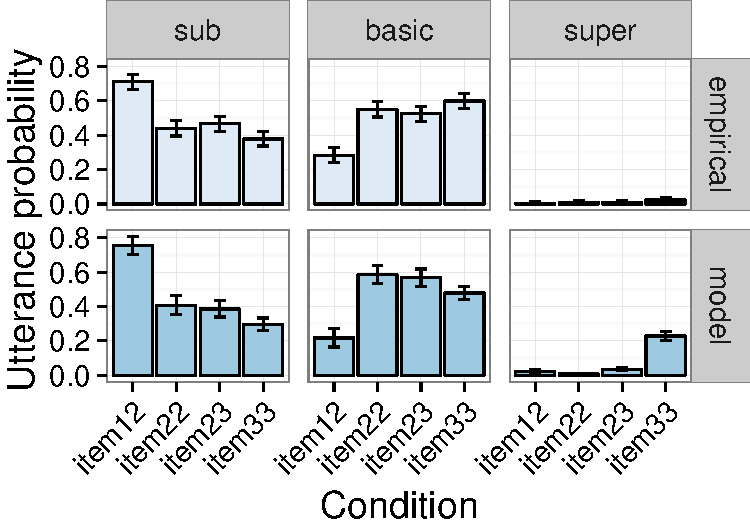
\includegraphics[width=.7\textwidth]{../../../models/old/5d_bda_nom_full/graphs/qualitativepattern-fulldataset-typicalities-hmc}
\caption{Utterance probabilities across different conditions. Columns indicate utterances, rows indicate data type (empirical proportion, MAP estimates of posterior predictives for full model with cost and non-deterministic semantics.}
\label{fig:exp2results}
\end{figure}

What explains these preferences? In order to test for effects of informativeness, length, frequency, and typicality on nominal choice we conducted a mixed effects logistic regression predicting sub over basic level mention from centered predictors for the factors of interest and the maximal random effects structure that allowed the model to converge (random by-speaker and by-target intercepts). 

\emph{Frequency} was coded as the difference between the sub and the basic level's log frequency, as extracted from the Google Books Ngram English corpus ranging from 1960 to 2008. 

\emph{Length} was coded as the ratio of the sub to the basic level's length. We used the mean empirical lengths in characters of the utterances participants produced. For example, the minivan, when referred to at the subcategory level, was sometimes called ``minivan'' and sometimes ``van'' leading to a mean empirical length of 5.71. This is the value that was used, rather than 7, the length of ``minivan''. That is, a higher frequency difference indicates a \emph{lower} cost for the sub level term compared to the basic level, while a higher length ratio reflects a \emph{higher} cost for the sub level term compared to the basic level.\footnote{We replicate the well-documented negative correlation between length and log frequency ($r = -.49$ in our dataset).} 

\emph{Typicality} was coded as the ratio of the target's sub to basic level label typicality.\footnote{Typicalities were elicited in a separate norming study that was identical in procedure to that of Exp.~1a. See \appref{app:typicalitynorms2} for details about the study.} That is, the higher the ratio, the more typical the object was for the sub level label compared to the basic level; or in other words, a higher ratio indicates that the object was relatively atypical for the basic label compared to the sub label. For instance, the panda was relatively atypical for its basic level ``bear'' (mean rating 0.75) compared to the sub level term ``panda bear'' (mean rating 0.98), which resulted in a relatively \emph{high} typicality ratio.

\emph{Informativeness} condition was coded as a three-level factor: \emph{sub necessary}, \emph{basic sufficient}, and \emph{super sufficient}, where item22 and item23 were collapsed into \emph{basic sufficient}. Condition was Helmert-coded: two contrasts over the three condition levels were included in the model, comparing each level against the mean of the remaining levels (in order: \emph{sub necessary}, \emph{basic sufficient}, \emph{super sufficient}). This allowed us to determine whether the probabilities of type mention  for neighboring conditions were significantly different from each other, as suggested by \figref{fig:exp2results}.

%\begin{table}[!tbp]
%\begin{center}
%\begin{tabular}{lrrl}
%\toprule
%\multicolumn{1}{l}{}&\multicolumn{1}{c}{Coef $\beta$}&\multicolumn{1}{c}{SE($\beta$)}&\multicolumn{1}{c}{$p$}\tabularnewline
%\midrule
%Intercept&$-0.02$&$0.27$&\textgreater 0.93\tabularnewline
%Condition sub.vs.rest&$ 2.05$&$0.17$&\textbf{\textless .0001}\tabularnewline
%Condition basic.vs.super&$ 0.54$&$0.15$&\textbf{\textless .001}\tabularnewline
%Frequency&$ 0.07$&$0.10$&\textgreater 0.5\tabularnewline
%Length&$-0.95$&$0.27$&\textbf{\textless .001}\tabularnewline
%Typicality&$ 4.84$&$1.32$&\textbf{\textless .001}\tabularnewline
%\bottomrule
%\end{tabular}\end{center}
%
%\end{table}

The log odds of mentioning the sub level term were greater in the \emph{sub necessary} condition than in either of the other two conditions ($\beta = 2.05$, $SE = .17$, $p < .0001$), and greater in the \emph{basic sufficient} condition than in the \emph{super sufficient} condition ($\beta = .54$, $SE = .15$, $p < .001$), suggesting that the contextual informativeness of the sub level mention has a gradient effect on utterance choice.\footnote{Importantly, model comparison between the reported model and one that subsumes basic and super under the same factor level revealed that the three-level condition variable is justified ($\chi ^2 (1) = 12.82$, $p < .0004$), suggesting that participants don't simply revert to the basic level unless contextually forced not to.} There was also a main effect of typicality, such that the sub level term was preferred for objects that were more typical for the sub level compared to the basic level  description ($\beta = .4.84$, $SE = 1.32$, $p < .001$, see \figref{fig:exp2effects}). In addition, there was a main effect of length, such that as the length of the sub level term increased compared to the basic level term (``chihuahua''/``dog'' vs.~``pug''/``dog''), the sub level term was dispreferred (``chihuahua'' is dispreferred compared to ``pug'', $\beta = -.95$, $SE = .27$, $p < .001$, see \figref{fig:exp2effects}). The main effect of frequency did not reach significance ($\beta = .07$, $SE = .10$, $p < .51$).

\begin{figure}
\centering
\includegraphics[width=\textwidth]{pics/lengthtypicality}
\caption{Proportion of sub level (over sub and basic level) terms across conditions. Left: when the sub  length is relatively short (.67,1.82] or long [1.82,4.3) compared to the basic level term. Right: when the target object was relatively more [1.06,1.91) or less (.88,1.06] typical for the sub compared to the basic level term. Intervals were generated by splitting data into groups of roughly equal numbers of observations.}
\label{fig:exp2effects}
\end{figure}


Unsurprisingly, there was also significant by-participant and by-domain variation in sub level term mention. %\figref{fig:bigscatterplot} shows the by-domain variation in utterance choice. 
For instance, mentioning the sub over the basic level term was preferred more in some domains (e.g. in the ``candy'' domain) than in others. Likewise, some domains had a greater preference for basic level terms (e.g. the ``shirt'' domain). Using the super term also ranged from hardly being observable (e.g. the ``flower'' domain) to being used more frequently (e.g. in the ``table'' and ``car'' domain). 

We thus replicate the well-documented preference to refer to objects at the basic level, which is partly modulated by contextual informativeness and partly a result of the basic level term's cognitive cost and typicality compared to its sub level competitor. 

Perhaps surprisingly given the previous literature, we did not observe an effect of frequency on sub level term mention. This may have a number of reasons. For instance, the modality of the experiment may have mattered here: the current study was a written production study, while most studies that have identified frequency as a factor governing production choices are spoken production studies (\red{cite cite}). It may be that the cognitive cost of typing longer words may be disproportionately higher than that of producing longer words in speech, thus obscuring a potential effect of frequency. 

\subsection{Non-deterministic RSA for nominal choice}
\label{sec:reflevelmodel}

Here we show that non-deterministic RSA as presented in \sectionref{sec:modifiedmodel} can be straightforwardly extended to modeling the choice of taxonomic level of reference. We include three modifications, while leaving the general framework as is. The first modification concerns the utterance alternatives. The second concerns the elicited typicality values and the resulting fidelity values. The third concerns the cost function. We briefly elaborate on each in turn. 

\paragraph{Utterance alternatives.} Whereas the modifier choice model treats all individual features and feature combinations represented in the display as utterance alternatives, the nominal choice model considers only the three different levels of reference to the target as alternatives, e.g., \emph{dalmatian}, \emph{dog}, \emph{animal}. That is, assuming a German Shepherd as a distractor, \emph{German Shepherd} is \emph{not} considered an alternative. This has consequences for the assumed fidelity values, which we turn to next. \jd{we should probably discuss this in the GD? ie, if we also assumed distractor labels as alternatives, we would have to do the rescaling -- would results be different? or the othe rway round: if we assume in modifier choice only the target's features are available as alternatives, would results be different?}

\paragraph{Fidelity values.} Just as we did for capturing color typicality effects in \sectionref{sec:modelevalcolortypicality}, we elicited empirical typicality values for object-utterance combinations.\footnote{See \appref{app:typicalitynorms2} for details of typicality elicitation experiment.} For each display, we know the typicality of each object in the display as an instance of the three potential target utterances (capturing, for instance, that the word ``dog'' describes a dalmatian better than a grizzly bear, but it also describes a grizzly bear better than a tennis ball). This allows us to use the typicality values as fidelity values directly, without rescaling as was necessary in the modifier choice model.

\paragraph{Cost function.} Recall the pragmatic speaker's utility function from \sectionref{sec:modifiedmodel}, where the weighted informativeness term $\alpha \ln P_{L_0}(o | u)$ traded off against the weighted utterance cost $\beta_c c(u)$. In the modifier model we assumed a constant cost for each added modifier. Because all utterance alternatives in the nominal choice model have word length 1, we update the cost function to be composed of each utterance's length $\hat{c}_l$ and frequency $\hat{c}_f$ (as described in the previous section), weighted by free parameters $\beta_f$ and $\beta_l$ :
\begin{equation}
P_{S_1}(u | o) \propto e^{\alpha \ln P_{L_0}(o | u) + \beta_f \hat{c}_f  + \beta_l \hat{c}_l)}
\end{equation}

To understand the qualitative behavior of the model, we briefly delve into two aspects of the model: first, the effect of typicality on the literal listener (and, in consequence via the pressure to be informative) the speaker. And second, the effect of cost (utterance length and frequency) on the speaker.

\subsubsection{Typicality effects}

\paragraph{Literal listener behavior.} The literal listener's probability of choosing the target under different typicalities for the observed utterance are shown in \figref{fig:nominallistenertypicality}. In general: as the target's typicality as an instance of the utterance increases and the distractors' typicality decreases, the probability of the literal listener choosing the target increases. Subordinate level terms tend to fall in the upper right quadrant of this graph. Basic level terms in the \emph{sub necessary} conditions tend to fall in the lower right quadrant, while basic level terms in the \emph{basic sufficient} conditions tend to fall in the upper right quadrant as well.

\begin{figure}
\centering
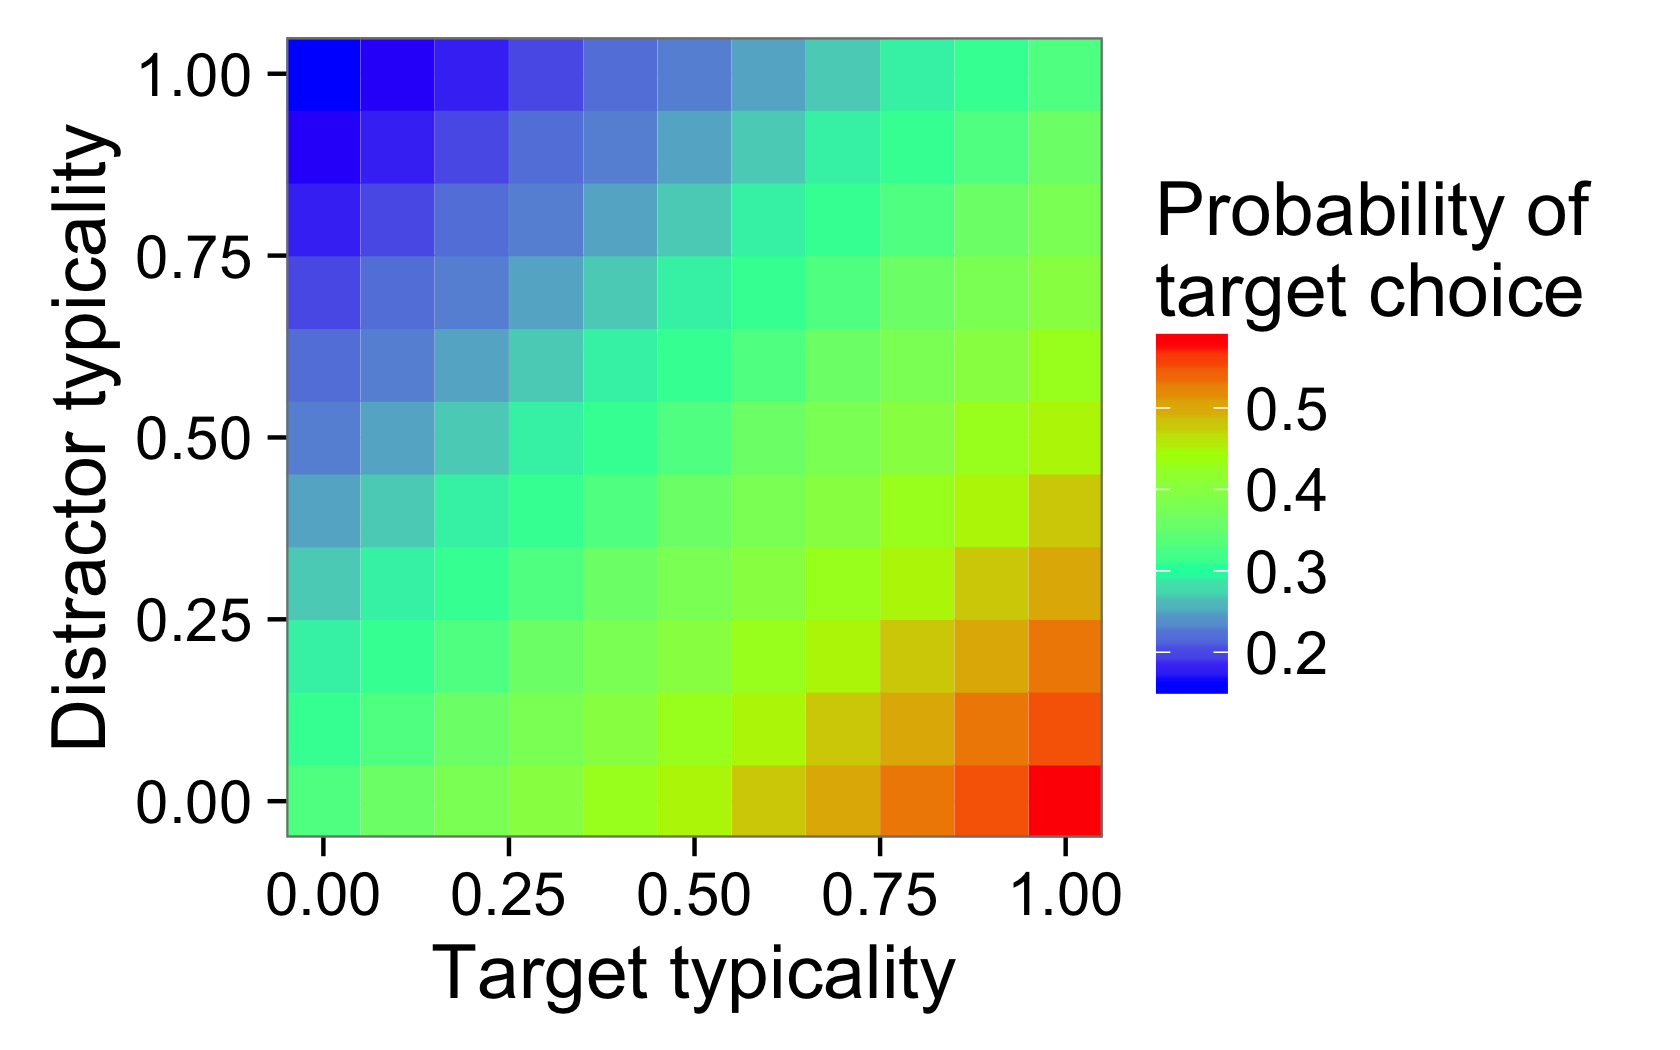
\includegraphics[width=.6\textwidth]{../../../models/old/6_qualitative_nom_L0/L0probs.png}
\caption{Literal listener probability of choosing the target under different typicalities of the target (x-axis) or the distractors (y-axis for the observed utterance. For simplicity we assume equal typicality of both distractors. The remaining probability mass for each case is thus uniformly distributed over both distractors.\jd{say where sub/basic/super level terms tend to fall in heatmap once you've regenerated plot}}
\label{fig:nominallistenertypicality}
\end{figure}

\paragraph{Pragmatic speaker behavior.} To understand the effect of typicality on the speaker's behavior it is useful to think about the problem of deciding which taxonomic level to refer at in terms of typicality gain, as we did in \sectionref{sec:colortypicality} for the choice between modified and unmodified expression. There, we found that relatively large target (compared to distractor) typicality gains in going from unmodified to modified expressions compared resulted in greater probability of overmodification. Here we observe the same effect in going from a higher (less specific) to a lower (more specific) taxonomic level. This can be seen in \figref{fig:nominalspeakertypicality}, which shows the probability of each utterance (sub, basic, or super) as a function of absolute target typicality as well as target typicality gain. Target typicality gain is the difference between the target's sub level typicality and the target's basic level typicality. Probabilities are shown for contexts with three items, always assuming $\alpha = 7$, but manipulating distractor typicality to simulate conditions analogous to our experimental conditions \emph{sub necessary}, \emph{basic sufficient}, and \emph{super sufficient}. Simulated distractor typicalities for sub, basic, and super level reference are shown in \tableref{tab:simulatedtyps}.

\begin{figure}
\centering
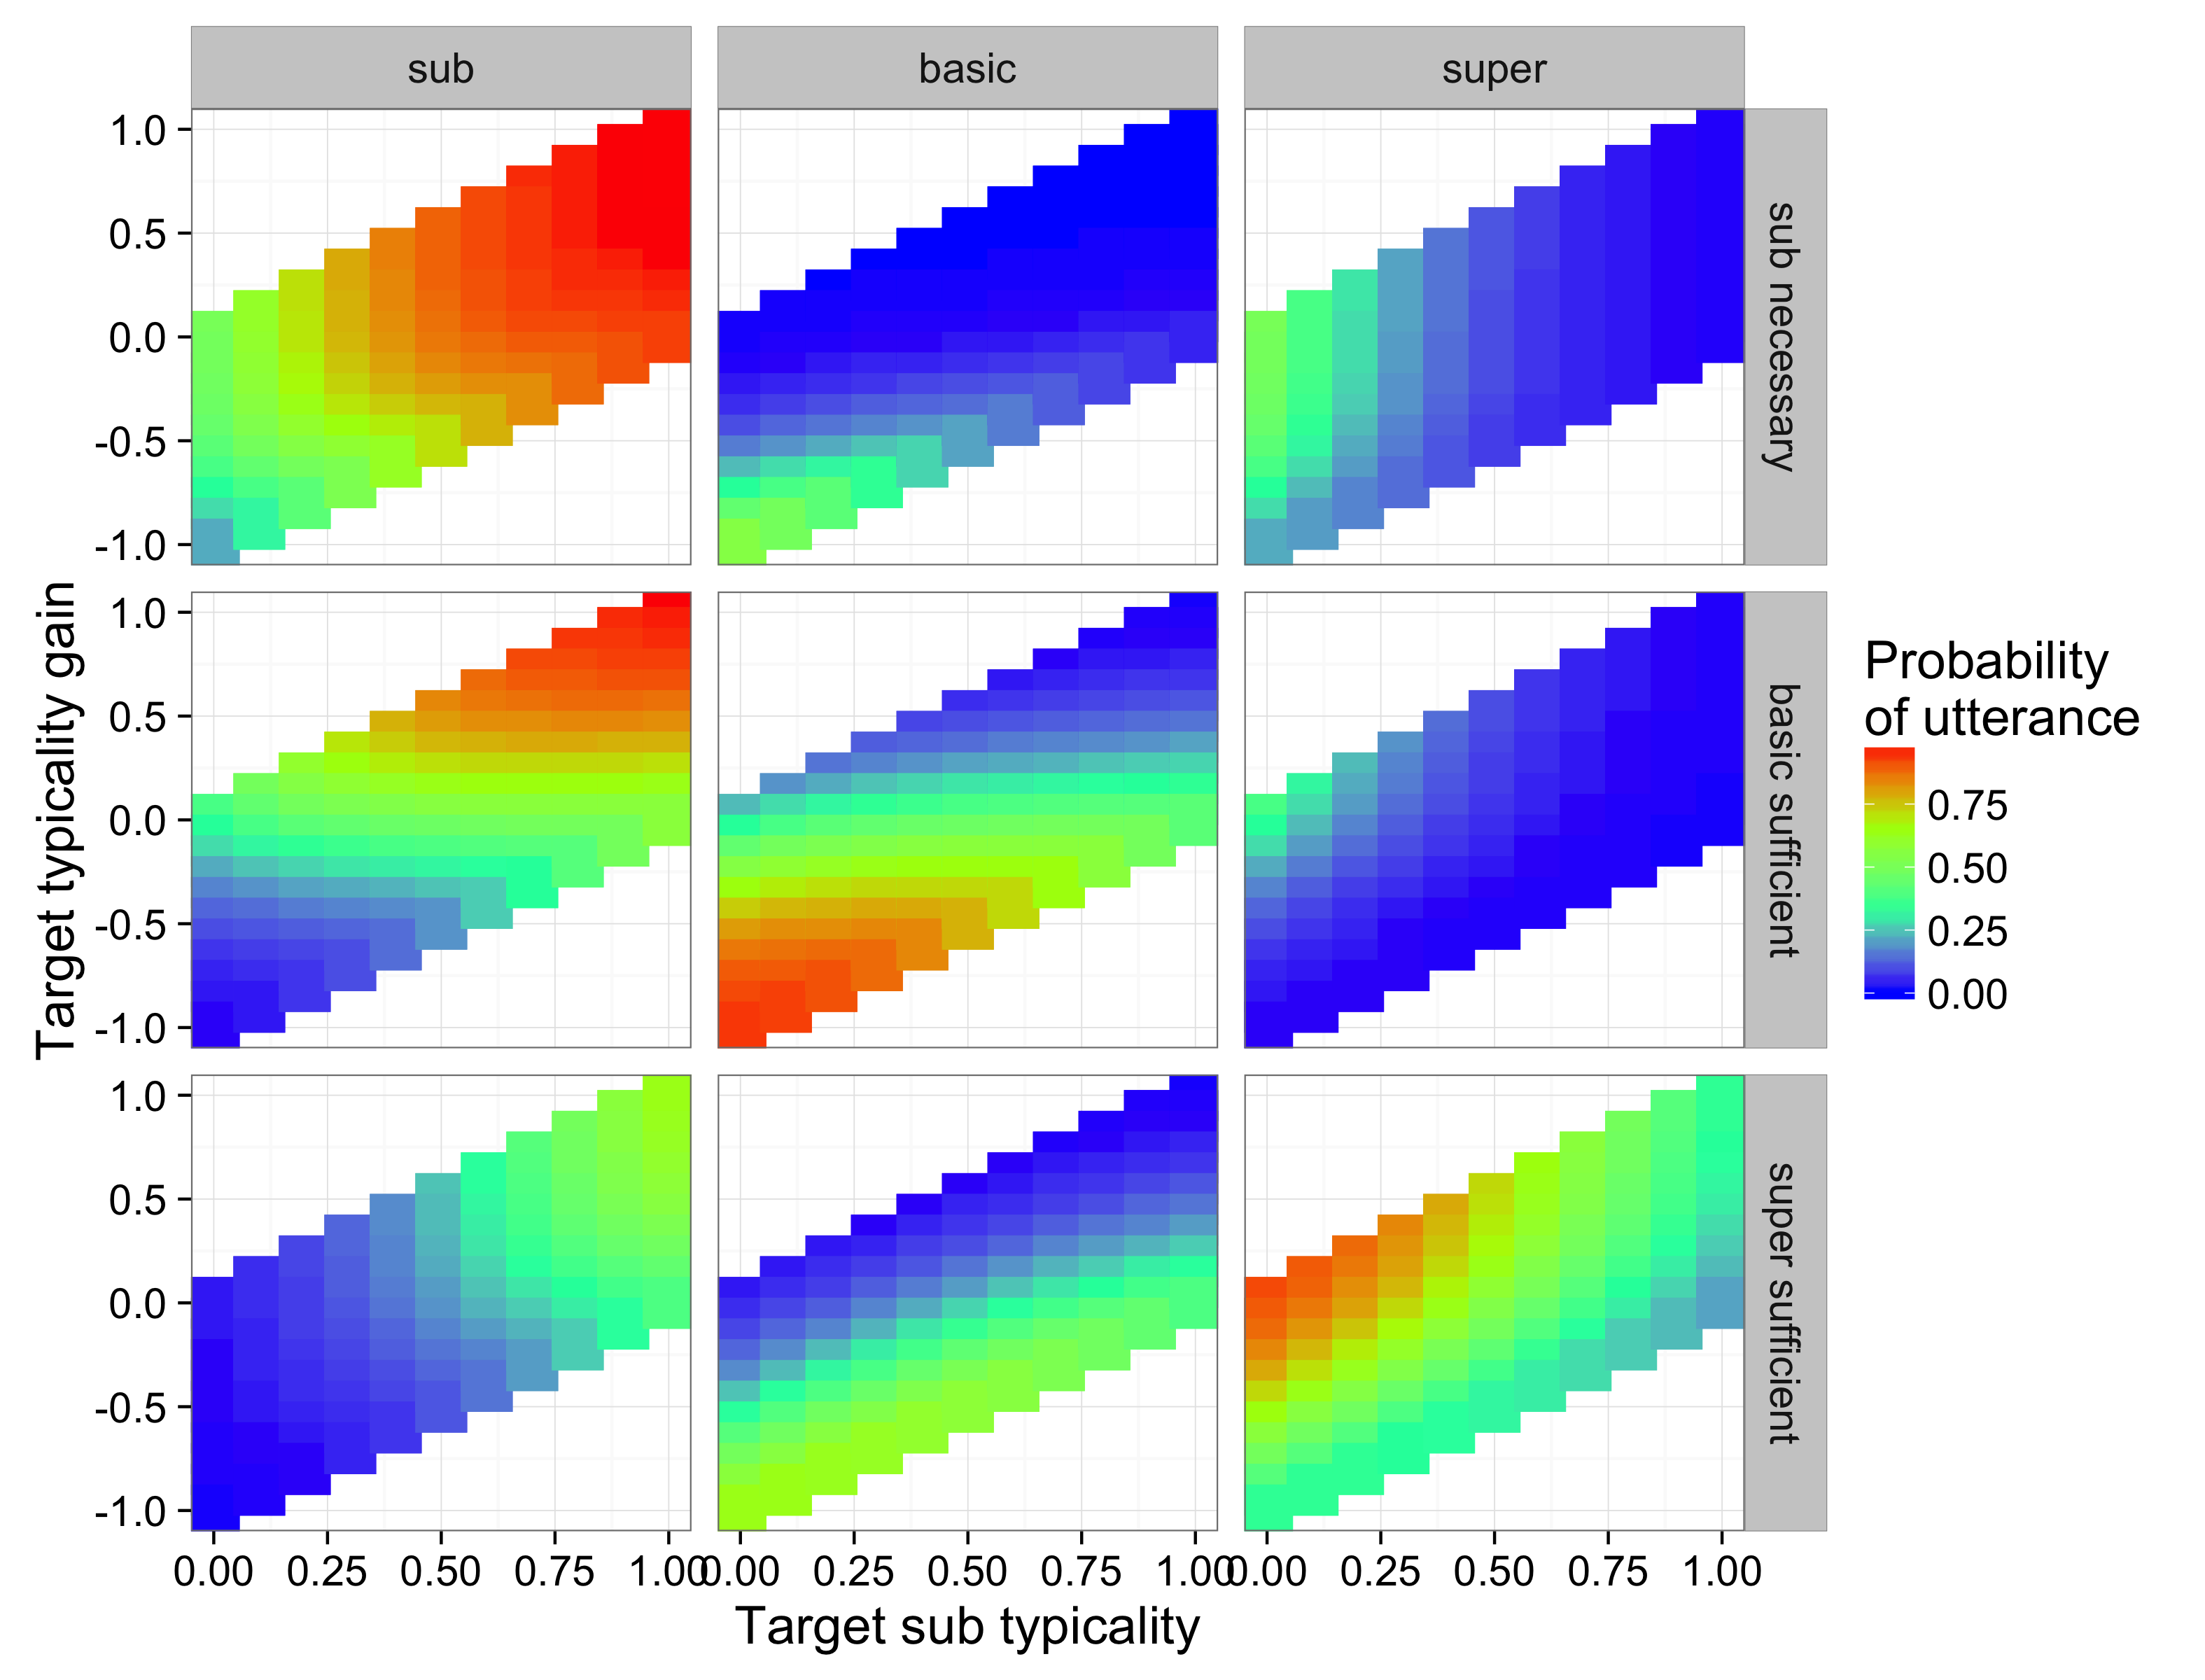
\includegraphics[width=\textwidth]{../../../models/old/7_qualitative_nom_S1_typ/S1probs_typgainmap_alpha7.png}
\caption{Pragmatic speaker probability of choosing each utterance (sub, basic, super) under varying absolute target sub typicalities (x-axis) and target typicality gains (difference between sub and basic level term typicality, y-axis), assuming equal typicality values for both distractors. Rows indicate different simulated conditions.\jd{go back into script to see how you computed typicality gain here}}
\label{fig:nominalspeakertypicality}
\end{figure}

\begin{table}
\centering
\caption{Overview of simulated distractor typicality (fidelity) values for sub, basic, and super level utterances in simulated conditions. In contrast to the actual experimental conditions, we assume equal typicality values for both distractors.}
\begin{tabular}{l l c c c}
\toprule
& & \multicolumn{3}{c}{Condition}\\
& & sub necessary & basic sufficient & super sufficient\\
\midrule
\multirow{3}{*}{Utterance} & sub & 0 & 0 & 0 \\
& basic & .8 & .1 & 0 \\
& super & .8 & .8 & 0\\
\bottomrule
\end{tabular}
\label{tab:simulatedtyps}
\end{table}

The blue areas in the graph indicate highest-probability regions. For example, as expected in the \emph{sub necessary} condition, the sub level term is the most likely one. However, in certain cases the basic level term also receives non-zero probability, notably when the target is a better instance of the basic than the sub level term, or (not pictured) when the typicality of the distractor as an instance of the basic level term is very low  (e.g., the typicality of the koala bear as an instance of "bear" was only 0.50). Indeed, the grizzly (with high typicality for basic level ``bear'', .97) is referred to as ``bear'' rather than ``grizzly bear'' in 85\% of \emph{sub necessary} conditions when the koala is the distractor. 

In the \emph{basic sufficient} conditions, sub level reference is nevertheless strongly predicted when target sub typicality gain is positive (i.e., when the target is a much better instance of the sub than of the basic level term). An example of such a case is the panda bear, who received a sub level typicality of .98 and a basic level typicality of only .75. Indeed, even when basic level reference was sufficient, the panda was referred to as the ``panda'' 81\% of the time.

These patterns mirror the typicality effects obtained via the mixed effects regression.


\subsubsection{Cost effects}

The additional effect of cost on nominal choice is straightforward: the costlier an utterance (relative to its alternatives), the less likely it is to be used. This pattern, too, is one observed in the mixed effects regression. For instance, the (short, less costly) pug is almost three times as likely as the (long, more costly) German Shepherd to be referred to by its subordinate level term in the \emph{basic sufficient} and \emph{super sufficient} conditions, where subordinate level reference is unnecessary. 

\bigskip
In \sectionref{sec:reflevelmodel} we showed that non-deterministic RSA captures the right kinds of qualitative effects as observed in the mixed effects regression. In the next section we evaluate how well the model captures nominal choice preferences quantitatively.

\subsection{Model evaluation: nominal choice}
\label{sec:reflevelmodeleval}

In order to evaluate non-deterministic RSA for nominal choice, we repeated the same Bayesian data analysis as reported in \sectionref{sec:modifiermodeleval} and \sectionref{sec:modelevalcolortypicality} to generate model predictions and infer likely parameter values. We did so by conditioning on the observed production data (coded into \emph{sub}, \emph{basic}, and \emph{super} level mentions as described above) and integrating over the three free parameters $\alpha  \sim \mathcal{U}(0,20)$, $\beta_f  \sim \mathcal{U}(0,5)$, $\beta_l  \sim \mathcal{U}(0,5)$.


Point-wise maximum a posteriori (MAP) estimates of the model's posterior predictives for each combination of utterance and informativeness condition (collapsing across different items) are compared to empirical data in \figref{fig:exp2results}. The model clearly captures the preference towards sub level mentions in the \emph{sub necessary} conditions and the basic level preference in all other conditions. It also captures the further decrease in sub level mentions in the \emph{super sufficient condition}. However, it does overpredict super level mentions, though not as badly as models that either assume a deterministic semantics or that ignore utterance cost.\footnote{The reader is referred to \appref{app:nominalmodelcomparison} for a comparison of the models containing a) only informativeness with deterministic semantics; b) only informativeness with non-deterministic semantics; c) informativeness with deterministic semantics and cost; d) informativeness with non-deterministic semantics and cost (the current model).} At this level, the model achieves a correlation of $r = .94$. Computing correlations additionally on the by-target level yields a correlation of $r = .84$ (see also the scatterplot in \figref{fig:exp2scatter}). 

\begin{figure}
\centering
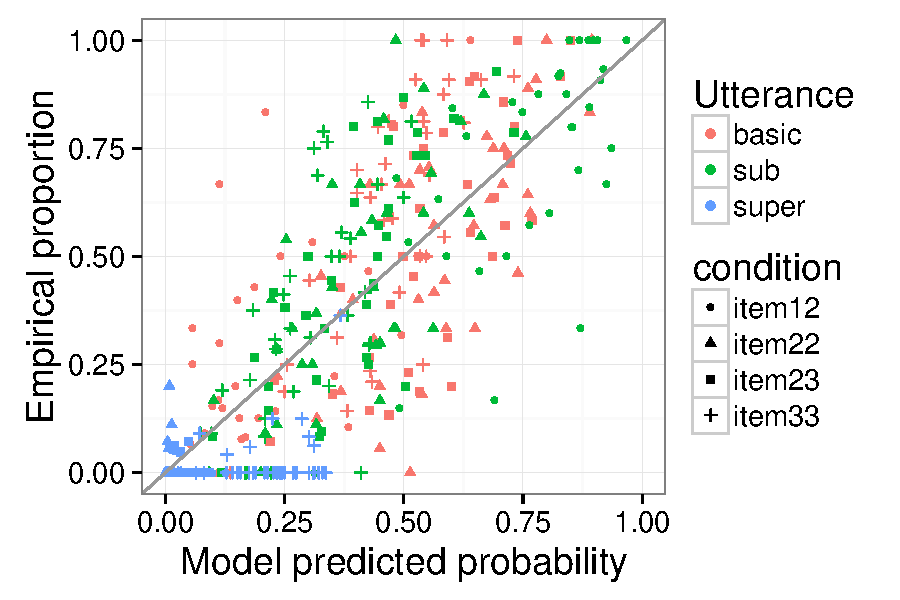
\includegraphics[width=.7\textwidth]{../../../models/old/5d_bda_nom_full/graphs/scatterplot-fulldataset-typicalities-hmc}
\caption{Scatterplot of by-target empirical utterance proportions against model posterior predictive MAP estimates. Gray line indicates perfect correlation line.}
\label{fig:exp2scatter}
\end{figure}

Parameter posteriors are shown in \figref{fig:nominalparamposteriors}. Both informativeness and length receive significant weight. In contrast, the effect of frequency appears to be much weaker with a MAP of .1 and the HDIs overlapping with 0. This mirrors the null effect of frequency found in the regression analysis. However, a large number of cases also received a non-zero frequency weight.

In order to ascertain whether typicality as incorporated in the non-deterministic semantics was indeed contributing to the explanatory power of the model, we ran an additional Bayesian data analysis with an added typicality weight parameter $\beta_t \in [0, 1]$. This parameter interpolated between empirical typicality values (when $\beta_t = 1$) and deterministic (i.e., 0 or 1) a priori values based on the true taxonomy (when $\beta_t = 0$). We found a MAP estimate for $\beta_t$ of .95, HDI = [0.82,.99], strongly indicating that it is useful to incorporate empirical typicality values and thus providing further support for the value of non-deterministic truth functions in modeling referring expressions.

\begin{figure}
\centering
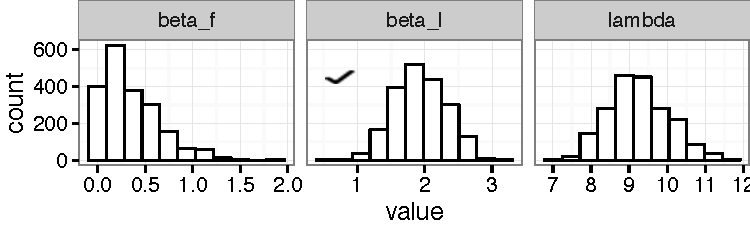
\includegraphics[width=.9\textwidth]{../../../models/old/5d_bda_nom_full/graphs/parameterposteriors-fulldataset-typicalities-hmc}
\caption{Posterior distribution over model parameters. Maximum a posteriori (MAP)  $\beta_f$ = 0.10, 95\% highest density interval (HDI) = [0.002,0.95]; MAP $\beta_l$ = 1.85, HDI = [1.23,2.65]; MAP $\alpha$ = 9.19, HDI = [7.72,10.80].}
\label{fig:nominalparamposteriors}
\end{figure}


%This relationship is motivated by considering the effect of a small difference in typicality on choice probability: in our elicitation experiment a small difference in rating should mean the same thing at the top and bottom of the scale (it is visually equivalent on the slider that participants used). In order for a small difference in typicality rating to have a constant effect on relative choice probability (which is a ratio), the relationship must be exponential. 


\section{General Discussion}
\label{sec:gd}

\begin{table}
\caption{Differences across model structures.}
\begin{tabular}{l l l l }
\toprule
& Color/size & Color typicality & Nominal choice \\
\midrule
Cost function & \jd{?} & empirical & empirical \\
Set of alternatives & contextually available & contextually available & target alternatives\\
Grammatical penalty & \jd{none?} & \jd{yes?} & none \\
\jd{Typicality weight} & none & \jd{yes?} & \jd{yes?}\\
\bottomrule
\end{tabular}
\label{tab:modeldiffs}
\end{table}

\jd{make sure to include adele goldberg's typicality effects in kids' generalizations to the basic level in discussion (srcd poster and submitted manuscript with lauren emberson)}

\subsection{Summary}

How do speakers choose a referring expression? Here we have shown that they do so by trading off various factors: the contextual informativeness of the referring expression on the one hand, and the cognitive cost of the expression on the other. Importantly, computing contextual informativeness with respect to a \emph{non-deterministic} underlying semantics was crucial for capturing various aspects of speakers' referring behavior. First, the non-deterministic semantics allowed us to capture the basic well-documented asymmetry for speakers to be more likely to redundantly use color adjectives rather than size adjectives. In addition, it predicted an interaction between sufficient dimension and scene variation on the probability of redundancy, which was very clearly borne out in the data: increased scene variation resulted in a much greater increase in redundant color than in redundant size adjective use. Finally, the non-determinism in the semantics gave rise to well-documented effects of typicality in both modifier choice and noun choice. A modifier was more likely to be mentioned redundantly when the object was a substantially less good instance of the unmodified than of the modified expression. Analogously, a noun at a taxonomically lower level than necessary for establishing reference was more likely to be mentioned when the object was a substantially less good instance of the higher than of the lower level. 

We have thus shown that with one key innovation -- a non-deterministic semantics  -- one can retain the assumption that speakers rationally trade off informativeness and cost of utterances in language production. Rather than being wastefully overinformative, adding redundant modifiers or referring at a lower taxonomic level than strictly necessary \emph{is} in fact informative when the prima facie sufficiently informative expression is substantially noisier than its redundant/overly specific counterpart. This innovation thus not only provides a unified explanation for a number of key patterns within the overinformative referring expression literature that have thus far eluded a unified explanation; it also extends to the domain of nominal choice.

In the following we discuss a number of intriguing questions this work raises and avenues for future research that it suggests.

\subsection{`Overinformativeness'}

This work challenges the traditional notion of overinformativeness in the linguistic and psychological literature \cite{engelhardt2006a, others}. The reason that redundant referring expressions became interesting for psycholinguists to study is because they seem to constitute a clear violation of rational theories of language production. For example, Grice's Quantity-2 maxim, which asks of speakers to ``not make [their] contribution more informative than is required'' \cite{grice1975}, appears violated by any redundant referring expression -- if size is the only feature that distinguishes the target object from the rest, the mention of color seems more informative than required. 

This conception of (over-)informativeness assumes that all modifiers are born equal -- i.e., that there are no a priori differences in the utility of mentioning different properties of an object. Under this conception of modifiers, there are hard lines between modifiers that are and aren't informative in a context. However, what we have shown here is that under a non-deterministic semantics, a modifier that would be regarded as overinformative under the traditional conception may nevertheless add some information about the referent. In particular, the more visual variation there is in the scene and the less noisy the redundant modifier is compared to the modifier that selects the  dimension that uniquely singles out the target, the more information it adds about the referent, and the more likely it therefore is to be mentioned. This work thus challenges the traditional notion of utterance overinformativeness by providing an alternative that nicely captures the quantitative variation observed in speakers' production in a principled way while still assuming that speakers are aiming to be informative.


What, then, would count as an overinformative utterance under non-deterministic RSA? RSA shifts the bar for overinformativeness and turns it into a graded notion: the less expected the use of a redundant modifier is (given knowledge of, e.g., utterance noise, cost, scene variation, and typicality), 
the more the use of that modifier will be considered overinformative. 

\subsection{Comprehension}

While the account proposed in this paper is not directly concerned with predicting listeners' behavior in interpreting referring expressions, it can be extended to do so relatively straightforwardly. RSA models typically assume that listeners, in interpreting utterances, are doing so by reasoning about their model of the speaker. In this paper we have provided precisely such a model of the speaker. In what way should the predicted speaker probabilities enter into comprehension? Here we can make a direct connection to surprisal theory in sentence processing \cite{levy2008}, where it has been shown that the effort involved in processing a sentence is a function of how surprising that sentence is under the listener's language model. While in these studies surprisal is usually estimated from syntactically parsed corpora, here we are providing a speaker model from which we can derive estimates of \emph{pragmatic surprisal}. Generally, the more likely a redundant utterance is, the easier it should be to process in context. We have shown that redundant expressions are more likely than minimal expressions when the distinguishing dimension is relatively noisy and scene variation is relatively high. In situations like these, one would thus expect the redundant expression to be easier to process than in cases where the redundant expression is relatively less likely. 

Is there evidence that listeners do behave in accordance with this prediction? While we have not run processing studies ourselves, we can look into the literature. Indeed, there is evidence that in situations where the redundant modifier does provide some information about the referent, listeners are faster to respond and select the intended referent when they observe a redundant referring expression than when they observe a minimal one \cite{Arts2011,  Paraboni2007}. However, there is also evidence that redundancy sometimes incurs a processing cost: both \citeA{Engelhardt2011} and \citeA{Davies2013} (Exp.~2) found that listeners were slower to identify the target referent in response to redundant compared to minimal utterances. It is useful to examine the stimuli they used. In the Engelhardt et al study, there was only one distractor that varied in type, i.e., type was sufficient for establishing reference. This distractor varied either in size or in color. Thus, scene variation was very low and overinformative expressions therefore likely surprising. Interestingly, the incurred cost was greater for redundant size than for redundant color modifiers, in line with the RSA predictions that color should be generally more likely to be used redundantly than size. In the Davies et al study, the `overinformative' conditions contained displays of four objects which differed in type. Stimuli were selected via a production pre-test: only those objects that in isolation were not referred to with a modifier were selected for the study. That is, stimuli were selected precisely on the basis that redundant modifier use would be unlikely.

While the online processing of redundant referring expressions is yet to be systematically explored under the non-deterministic RSA account, this cursory overview of the patterns reported in the existing literature suggests that pragmatic surprisal (i.e., negative log-transformed speaker probabilities) may be a plausible linking function from model predictions to processing times.


%\jd{Interesting snippet from Pechmann which we may want to quote but is actually so misguided on his part that it may just be mean to include it: ``in information theory, a positive function is assigned to redundancy, since it can compensate for partial loss of information. Can overspecification in referential communication have the same function? We can rule out this possibility, because we regard those utterances as being `redundant' which include nondistinguishing features in addition to distinguishing ones. Yet nondistinguishing features cannot compensate for the loss of distinguishing information, since by definition nondistinguishing features do not distinguish the target referent from context. At best, they can reduce the domain of referential alternatives.'' $\rightarrow$ But that IS compensating!}

%
%The work reported here clearly shows that overmodified referring expressions, contrary to some claims in the literature \cite{Engelhardt2011} \red{who say overmodification ipmairs comprehension}, contribute more utility than `minimally' specified referring expressions.

\subsection{Fidelity}

The model crucially relies on a non-deterministic semantics to capture the effects we have reported in this paper. But what is the nature of this non-determinism? What does it represent? For the purpose of Exp.~1 (modifier choise), fidelity initially applied at the modifier \emph{type} level. The semantics of modifiers was underlyingly truth-conditional and the fidelity term captured the probability that a modifier's truth conditions would accidentally be inverted. This model included only two fidelity terms, one for size and one for color. We then extended the notion of fidelity to apply at the level of utterance-object  combinations (e.g., \emph{golf ball} vs.~\emph{pink golf ball} as applied to a pink golf ball) to account for color typicality effects. In this instantiation of the model, fidelity differed for every utterance-object combination and captured how good of an instance of an utterance an object was. Similarly, in Exp.~2 (nominal choice) fidelity differed for every utterance-object combination (e.g., \emph{dog} vs.~\emph{dalmatian} as applied to a dalmatian). This is summarized in \tableref{tab:fidelitynature}.

\begin{table}
\caption{Fidelity across models alongside the effects from \tableref{tab:effects} that each model captures.}
\begin{tabular}{l p{2.8cm} p{3cm} p{4cm} p{4.5cm}}
\toprule
Exp. & Model & Fidelity level & How obtained & Effect(s)\\
\midrule
1 & basic non-deterministic & modifier type & inferred & color/size asymmetry \& scene variation\\
1 & typicality (modified/unmodified) & utterance-object & elicited (nominal, color) and inferred (size) & color/size asymmetry, scene variation, \& color typicality\\
2 &  typicality (level of reference) & utterance-object & elicited & basic level preference \& subordinate level mention\\
\bottomrule
\end{tabular}
\label{tab:fidelitynature}
\end{table}

What we have said nothing about thus far is where these numbers come from; in particular, which aspects of our experience -- linguistic, perceptual, conceptual, communicative -- they represent. We will offer some speculative remarks and directions for future research here. 

First, it is possible that the numbers represent the difficulty associated with verifying whether the property denoted by the utterance holds of the object. This difficulty may be perceptual -- for example, it may be relatively easier to visually determine of an object whether it is red than whether it it is big. Similarly, at the object-utterance level, it may be easier to determine of a yellow banana than of a blue banana whether it exhibits banana-hood, in consequence yielding a lower typicality value for a blue banana than for a yellow banana as an instance of \emph{banana}. It may also be conceptual -- for example, it may be easier to determine whether a box belongs to John than whether \red{XXX}.

Another possibility is that the numbers represent aspects of agents' prior beliefs (world knowledge) about the correlations between features of objects. For example, conditioning on bananahood holding of objects and asking for the relative probabilities of various colors obtaining in that set will yield a high number for yellow and a low one for blue.\footnote{Though these probabilities cannot directly match up with the elicited typicality values, given that probabilities will have to sum up to 1, while typicality values were not normalized.} 

Another hypothesis is that the numbers capture the past probability of communicative success in using a particular utterance (e.g., \emph{banana}) to refer to an object with a particular set of features (e.g., blue bananas vs.~yellow bananas). However, this probability is likely itself not independent of the first two possibilities discussed.

Finally, it is also possible that the numbers are simply an irreducible part of the lexical entry of each utterance-object pair. This seems unlikely, given that this would require a separate number for each utterance and object token. It also suggests that the numbers should not be updated in response to further exposure of objects. For example, if the numbers were a fixed component of the lexical entry \emph{banana}, then even being exposed to a large number of blue bananas should not change the value. This seems unlikely but deserves to be investigated further. 


%\jd{from sec:modifierdiscussion: already bring up discussion points here? eg is it really about COLOR vs SIZE or particular color and size terms (blue vs turqoise), or about COLOR/blue for a particular object (ie typicality)? what about the issue that regularly comes up: that in context, surely these modifiers are not noisy?}

%\jd{from sec:modifierdiscussion: There is quite a bit of variation in the actual overmodification numbers in previous studies. Use that as a bridge to typicality and next section (you also say in intro that you're going to discuss this, so you better do it).} 


%nature of numbers in non-deterministic semantics (we see that typicality effects fall out of treating the numbers in the semantics as typicality values for noun choice, and the same if we make up values for modifier choice -- but how do we get here compositionally? one would ideally model the structure in the prior (rich world knowledge), ie the statistical correlations between different dimensions (type -- banana, color -- blue/yellow, etc) and have the fidelity/noise values emerge from THAT compositionally!


\subsection{Audience design}

One question which has plagued the literature on language production is that of whether, and to what degree, speakers actually tailor their utterances to their audience \cite{Clark1982, horton1996, Brown-schmidt2014}. This is also known as the question of \emph{audience design}. With regards to redundant referring expressions, the question is whether speakers produce redundant expressions because they can't help it (i.e., due to internal production pressures) or specifically because it is helpful for their interlocutor (i.e., due to considerations of audience design).

Non-deterministic RSA seems to make a claim about this issue: the non-determinism is located in the literal listener component, with respect to which speakers are trying to be informative. That is, it would seem that speakers produce referring expressions that are tailored to their listeners. However, this is misleading. The ontological status of the literal listener is as a ``dummy component'' that allows the pragmatic recursion to get off the ground. Actual listeners are, in line with previous work, more likely fall into the class of pragmatic $L_1$ listeners; listeners who reason about the speaker's intended meaning via Bayesian inference \cite{frank2012, goodmanstuhlmueller2013}.  

Because RSA is a computational-level theory \cite{marr1982} of language use, it does not claim that speakers \emph{actually, consciously} consult an�internal model of a listener every time they choose an utterance, just that the distribution of utterances they use reflect informativity with respect to such a model. It is possible that this distribution is cached or computed using some other algorithm that doesn?t explicitly involve a listener component. 

Thus, the RSA model as formulated here remains agnostic about whether speakers' (over-) informativeness should be considered geared towards listeners' needs or simply a production-internal process. 


\subsection{Other factors affecting redundancy}

Non-deterministic RSA as presented in this paper straightforwardly accounts for effects of typicality, cost, and scene variation on redundancy in referring expressions. However, other factors have been identified as contributing to redundancy. For example, \citeA{rubiofernandez2016} has shown that colors are mentioned more often redundantly for clothes than for geometrical shapes. Her explanation: knowing an object's color is generally more useful for clothing than it is for shapes. While she doesn't provide a detailed explanation for why this is the case, it is plausible that agents' knowledge of \emph{goals} may be relevant here. For example, knowing the color of clothing is relevant to the goal of deciding what to wear or buy. In contrast, knowing the color of geometrical shapes is rarely relevant to any everyday goal agents might have. While the RSA model as implemented here does not accommodate an agent's goals, it can be extended to do so via projection functions, as has been done for capturing figurative language use \cite<e.g.,>{kao2014} or question-answer behavior \cite{Hawkins2015}. This should be explored further in future research.


\jd{a note on incrementality? eg, pechmann says incrementality is to blame for redundancy: we retrieve words when we can, and colors are easier to retrieve, so we throw them out there regardless of whether or not they're redundant. The problem with this is that this makes a prediction about the order of adjectives; in particular, the preferred order should be reversed. Pechmann does find some instances of this, but not very many. But there are other ways incrementality could play a role. For example, throwing out the color word may help when the noun is hard to retrieve. This predicts that in languages with post-nominal adjectives, where you can't use this as a delay strategy for holding off on planning the noun, there should be less color redundancy; indeed, Rubio-Fernandez 2016 shows this for Spanish. The dynamic nature of language processing plays a role in other ways, too: it allows us to update our beliefs about individual speakers' use of modifiers and generate better expectations about upcoming input. For example, Pogue et al 2016 have shown that listeners, after being exposed to consistently overinformative speakers, stop drawing early contrastive inferences based on modifier use.}


\subsection{Extensions to other language production phenomena}

In this paper, we have focused on providing an account of content selection \cite{GattEtAl2013} in modified referring expressions on the one hand (i.e., when to mention an object's size or color) and in nominal referring expressions on the other (i.e., at which taxonomic level to refer to an object). Future work should investigate whether these  models can be merged to jointly account for the choice of content expressed in modifiers and in nouns. Further, in order to scale up to more naturalistic conversational domains it will be necessary to consider richer language models. Recall that we treated different color names (e.g., \emph{pink} and \emph{purple}) as simply a color mention. Similarly, we treated different nouns that clearly referred at the same level (e.g., \emph{grizzly} and \emph{grizzly bear}) as simple sub level mentions. For the purpose of predicting not only content selection but also utterance choice, a richer inventory of utterance alternatives will need to be explored. An interesting question is how this approach can be extended to other referring expressions mentioned in the Introduction, e.g., names, pronouns, or referring expressions with post-nominal modification.

However, future research should also investigate the very intriguing potential for this approach to be extended to any language production phenomenon that involves content selection. For example, there is a large literature on optional instrument mentions. \citeA{brown1987} showed that atypical instruments are more likely to be mentioned than typical ones -- if a stabbing occurred with an icepick, speakers prefer "The man was stabbed with an ice pick" rather than ``The man was stabbed''. If instead a stabbing occurred with a knife, ``The man was stabbed'' is preferred over "The man was stabbed with a knife"). This is very much parallel to the case of atypical color mention. While \citeA{brown1987}'s account of the effect is that speakers do or don't mention instruments for speaker-internal ego-centric reasons, later evidence suggests an explanation  that is rather more driven by audience design considerations. \citeA{lockridge2002} replicated the original finding in a story retelling scenario while also manipulating whether or not addressees saw pictures of the actions. Without pictures, speakers produced even more mentions of atypical objects (presumably to prevent addressees from forming a faulty mental model of the situation), suggesting that the typicality effect is in fact an audience design effect. 

More generally, the approach should extend to any content selection phenomenon that affords a choice between a more or less specific chunk of linguistic signal. Whenever the chunk adds sufficient information, it should be included. This is related to surprisal theories of production like Uniform Information Density \cite<UID,>{jaeger2006, levy2007, frank2008, jaeger2010}, where it has been found that speakers are more likely to omit linguistic signal if the underlying meaning or syntactic structure is highly predictable. Importantly, UID diverges from ours in that ours is (thus far) an account of \emph{content selection}, while UID is an account of the choice between meaning-equivalent alternative \emph{utterances}.


\subsection{Conclusion}
\label{sec:conclusion}

In conclusion, we have provided an account of redundant referring expressions that challenges the traditional notion of overinformativeness, unifies multiple language production literatures, and has the potential for many further extensions. For the time being, we take this work to suggest that, rather than being wastefully overinformative, speakers are rationally redundant.

\jd{What else needs to be included in GD?}

\appendix

\section{Effects of semantic value on utterance probabilities}
\label{app:modelexploration}

Here we visualize the effect of different adjective types' semantic value on the probability of producing the insufficient color-only utterance (\emph{blue pin}), the sufficient size-only utterance (\emph{small pin}), or the redundant color-and-size utterance  (\emph{small blue pin}) to refer to the target in context \figref{fig:sizesufficient} under varying $\alpha$ values, in \figref{fig:fullexploration}. This constitutes a generalization of \figref{fig:basicasymmetry}, which is duplicated in row 6 ($\alpha = 30$).

\begin{figure}
\centering
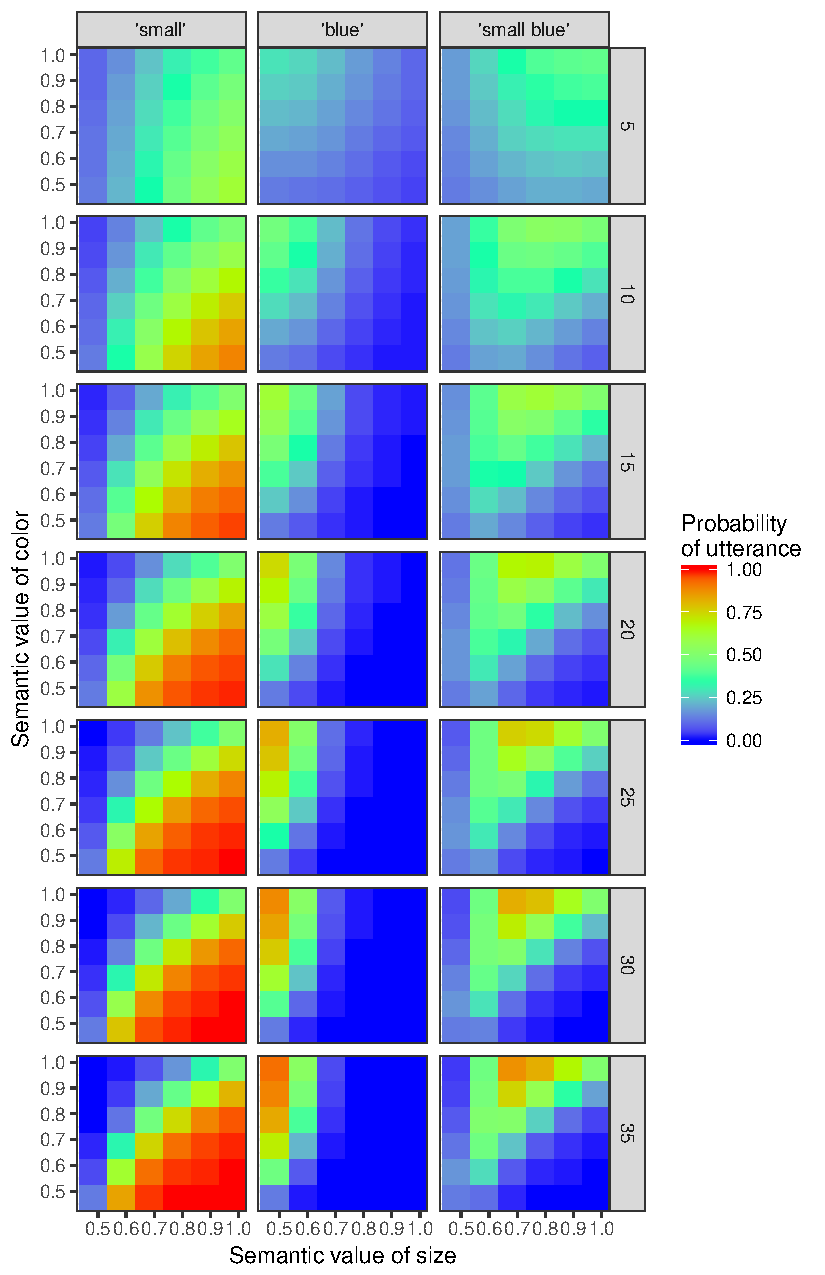
\includegraphics[width=.82\textwidth]{pics/modelexploration-fullfidelityeffect-unlogged-wide}
\caption{Probability of producing sufficient \emph{small pin}, insufficient \emph{blue pin}, and redundant \emph{small blue pin} in contexts as depicted in \figref{fig:sizesufficient}, as a function of semantic value of color and size utterances and varying $\alpha$ row-wise (for $ \beta_c = 0$).}
\label{fig:fullexploration}
\end{figure}

%\section{Model exploration for Koolen scene variation contexts}
%\label{app:koolenexploration}
%
%In \figref{fig:koolenfullexploration} we visualize model predicted probability of redundantly using color under varying $\alpha$ values (columns), color fidelity values (rows), and size fidelity values (x-axis), for the high and low variation conditions in their Exp.~1 (where type was sufficient for reference) and Exp.~2 (where type and size was necessary for reference). The assumed type fidelity is .9.
%
%\begin{figure}
%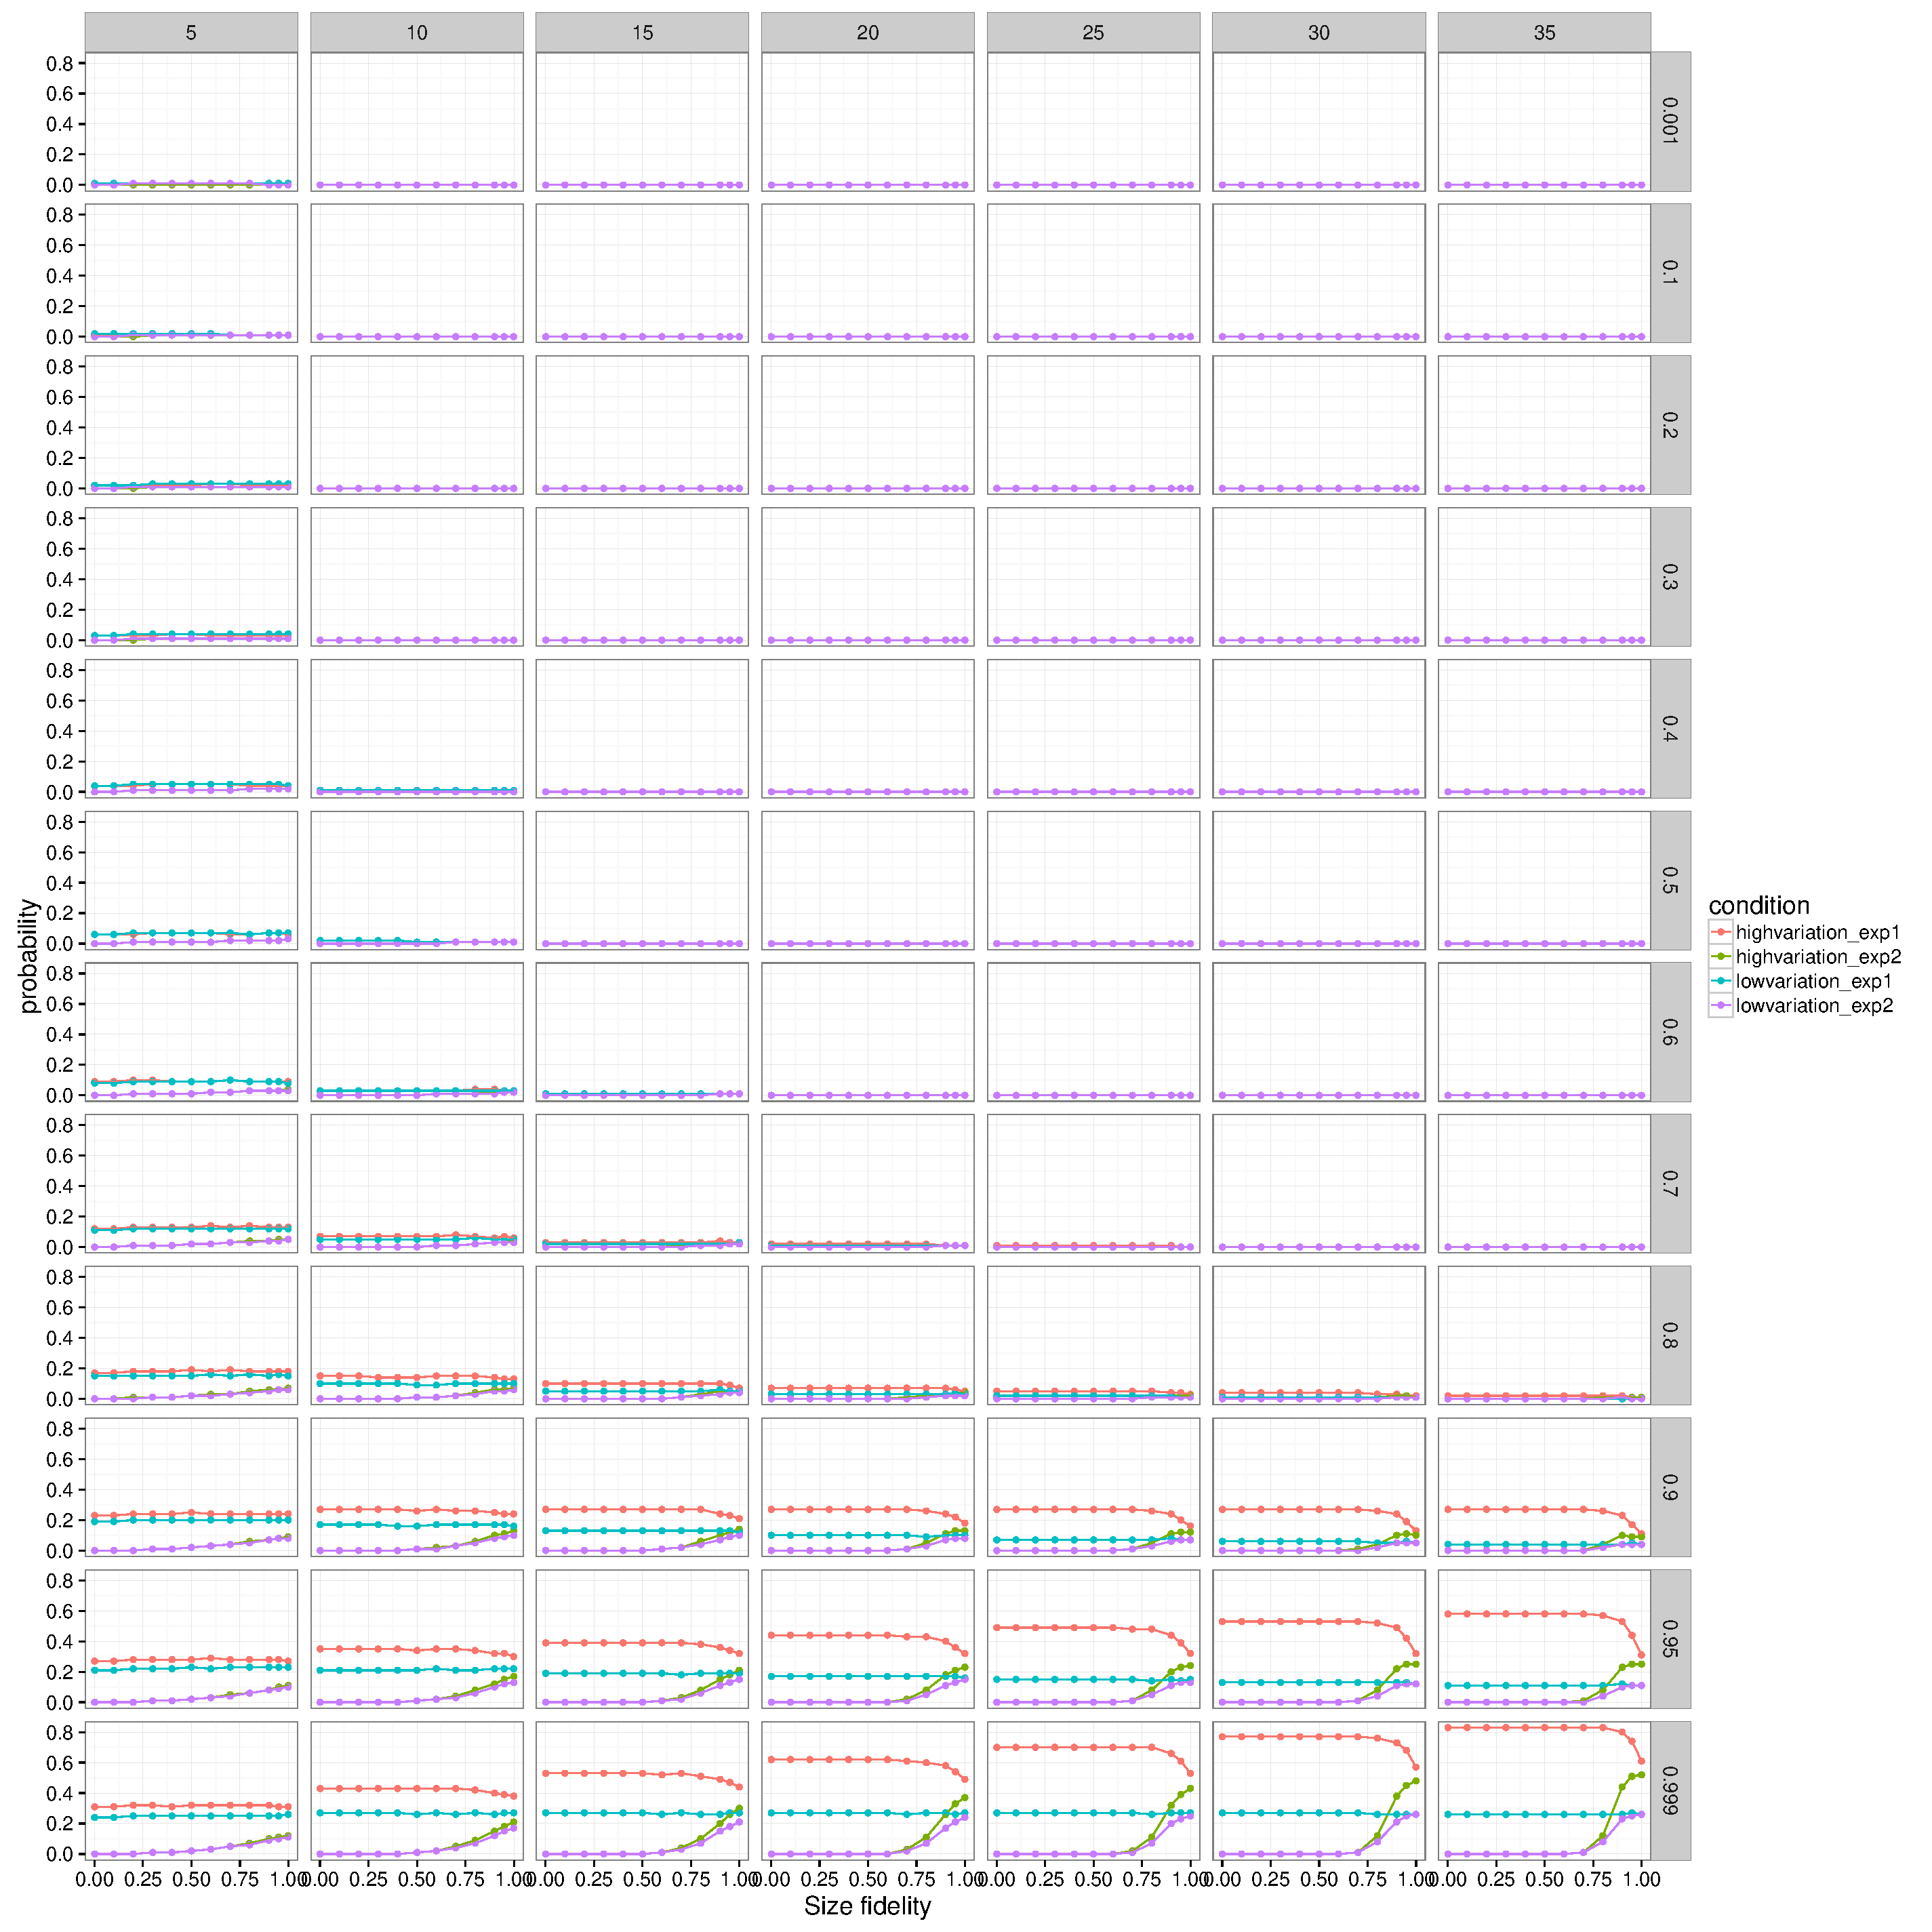
\includegraphics[width=\textwidth]{pics/koolen-full-exploration}
%\caption{Probability of redundant color mention as a function of size fidelity (x-axis), color fidelity (rows), and varying $\alpha$ (columns).}
%\label{fig:koolenfullfullexploration}
%\end{figure}


\section{Validation of interactive web-based written production paradigm}
\label{app:replication}

\red{make sure to discuss why overall we have lower overspecification rates -- probably because of color typicality!! we had pretty typical colors in our stimuli}

\section{Pre-experiment quiz}
\label{app:numdistractors}

Before continuing to the main experiment, each participant was required to correctly respond ``True'' or ``False'' to the following statements. Correct answers are given in parentheses after the statement.

\begin{itemize}
	\item The speaker can click on an object. (False)
	\item The listener wants to click on the object that the speaker is
  telling them about. (True)
  \item  The target is the object which has the red circle around it. (False)
  \item Only the speaker can send messages. (False)
  \item There are a total of 72 rounds. (True)
  \item The locations of the three objects are the same for the speaker and the listener. (False)
\end{itemize}


\section{Experiment 1 items}
\label{app:itemtypes}

The following table lists all 36 object types from Exp.~1 and the colors they appeared in:

\begin{tabular}{l l l l}
\toprule
Object & Colors & Object & Colors \\
\midrule
avocado & black, green & balloon & pink, yellow \\
belt & black, brown & bike & purple, red\\
billiard ball & orange, purple & binder & blue, green \\
book & black, blue & bracelet & green, purple \\
bucket & pink, red & butterfly & blue, purple\\
candle & blue, red & cap & blue, orange \\
chair & green, red & coat hanger & orange, purple \\
comb & black, blue & cushion & blue, orange\\
flower & purple, red & frame & green, pink \\
golf ball & blue, pink & guitar & blue, green\\
hair dryer & pink, purple & jacket & brown, green\\
napkin & orange, yellow & ornament & blue, purple\\
pepper & green, red & phone & pink, white\\
rock & green, purple & rug & blue, purple \\
shoe & white, yellow & stapler & purple, red\\
thumb tack & blue, red & tea cup & pink, white \\
toothbrush & blue, red & turtle & black, brown \\
wedding cake & pink, white & yarn & purple, red\\
\bottomrule
\end{tabular}

%\section{Analysis of cases with higher inferred size than color typicality}
%\label{app:fidelity-outliers}
%
%\figref{fig:fidelity-outliers-reducedconditions} visualizes all 10,000 samples' from the BDA run on the data from Exp.~1 with an eye towards understanding the cases in which inferred size fidelity was greater than color fidelity. In general, these cases were very unlikely, with a posterior probability of .048. Conditioning on these cases, the probability of a low cost weight was only .23 (only .01 probability overall). That is, where color fidelity was lower than size fidelity, the model tried to achieve the empirical color-size asymmetry by placing greater weight on cost differences, where size was always inferred to be costlier than color.
%
%\begin{figure}
%\centering
%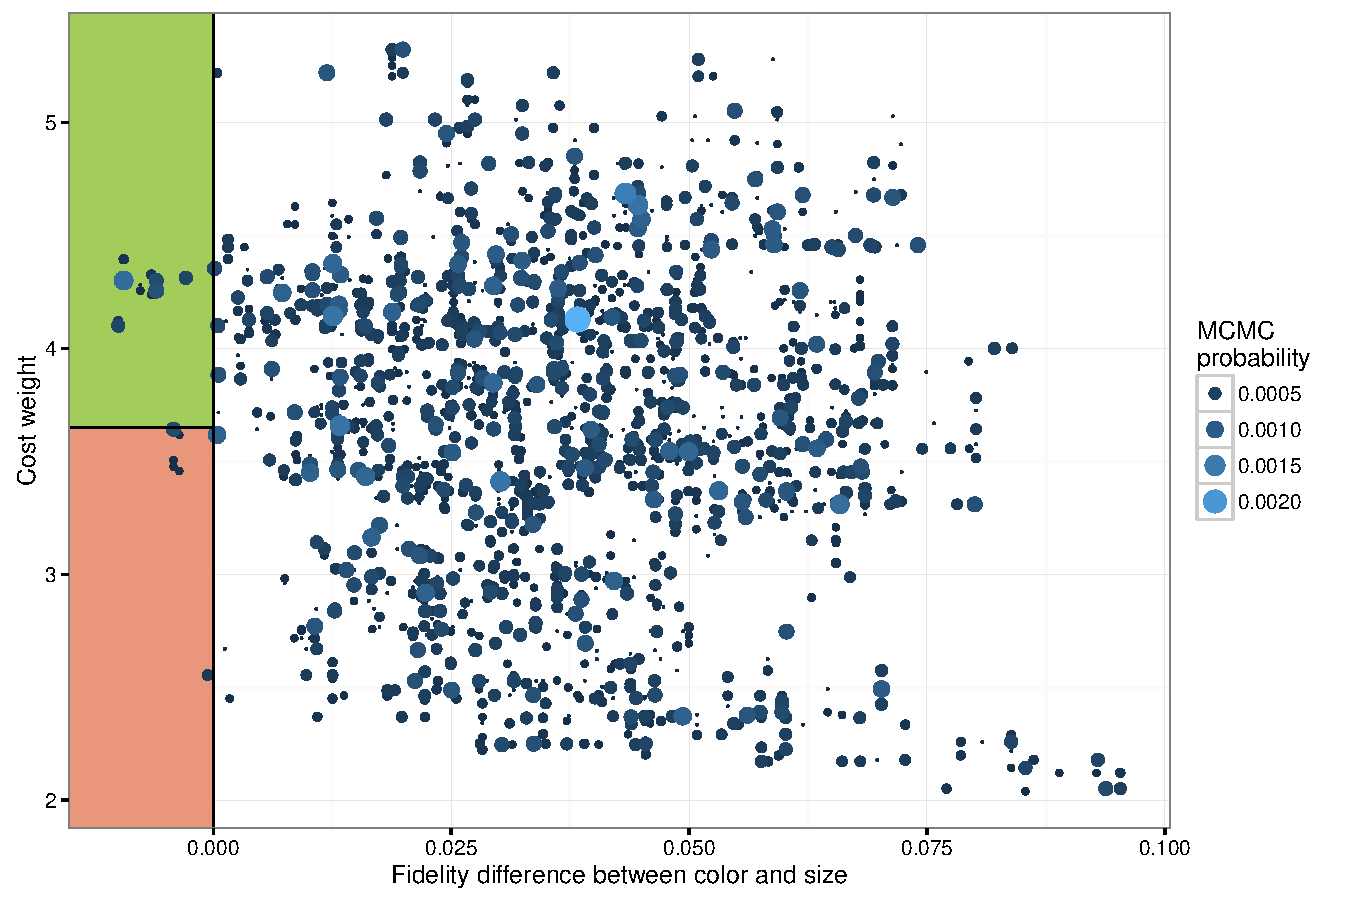
\includegraphics[width=.7\textwidth]{../../../models/1a_bda_basic/results_bda/graphs/fidelity-outliers-fixed-reducedconditions}
%\caption{Each sample's cost weight $\beta_c$ against difference between color and size fidelity ($f_{\textrm{c}} - f_{\textrm{s}}$). Green region includes cases with higher inferred size than color fidelity that have a cost weight greater than or equal to the median cost weight. Red region includes cases with higher inferred size than color fidelity that have a cost weight lower than the median cost weight. Dot size and color indicates parameter values' posterior probability.}
%\label{fig:fidelity-outliers-reducedconditions}
%\end{figure}

\section{Experiment 2a: typicality norms for Experiment 2}
\label{app:typicalitynorms2}

Analogous to the color typicality norms elicited for utterances in Exp.~1, we elicited typicality norms for utterances in Exp.~2. The elicited typicalities were used in the Bayesian Data Analysis reported in \sectionref{sec:reflevelmodeleval}.

\subsubsection{Methods}

\paragraph{Participants}

We recruited 240 participants over Amazon's Mechanical Turk who were each paid \$0.50 for their participation.

\paragraph{Procedure and materials}

On each trial, participants saw one of the images used in Exp.~2 and were asked to answer the question ``How typical is this for an \emph{X}?'' on a continuous slider with endpoints labeled ``very atypical'' to ``very typical.'' \emph{X} was a nominal referring expression. In contrast to Exp.~1a, where we only elicited typicality norms for utterance-object pairs where the object was in the extension of the utterance under a deterministic semantics (e.g., here\emph{dalmatian}, \emph{dog}, or \emph{animal} for a dalmatian), in this norming study we also elicited norms for utterance-object pairs where that was not clearly the case (e.g., \emph{a bear} for a bison, \emph{a car} for an ambulance, or \emph{a snack} for a lobster). However, we did not test all utterance-object combinations, which would have led to an explosion of conditions. Instead, we tested each target object with its three utterances (e.g., the dalamtian was paired with \emph{dalmatian}, \emph{dog}, and \emph{animal}; the pug was paired with \emph{pug}, \emph{dog}, and \emph{animal}, etc.). That yielded a total of 108 combinations -- four targets in nine domains with three utterances each. We further tested each distractor item that shared the target's superclass category (\emph{dist-samesuper}, e.g., cows share the superclass category animal with dogs) on both the basic level and the super level term (e.g., \emph{dog} for cow and \emph{animal} for cow), for a total of 469 combinations. Finally, we also tested each distractor of a different super category than the target on the target's super level term (\emph{dist-diffsuper}, e.g., \emph{animal} for socks). This yielded another 168 combinations. Overall, we obtained typicality norms for 745 object-utterance combinations. All other object-utterance combinations were assumed to have typicality 0.

Each participant rated 45 items: 7 targets, 10 dist-diffsuper, and 28 dist-samesuper cases. These were randomly sampled from the overall pool of items in each category. 

\subsubsection{Results and discussion}

Each combination was rated at least 5 times and at most 27 times. We coded the slider endpoints as 0 (``very atypical'') and 1 (``very typical''). In order to evaluate the model, we used each object-utterance combination's typicality mean as input. 

Typicality ratings by item type (target, dist-samesuper, dist-diffsuper) and utterance type (sub, basic, super) are visualized in \figref{fig:typicalityboxplots}. As expected, typicality was close to 0 for dist-diffsuper cases and for sub/basic terms used with dist-samesuper cases. However, even for these cases, there was some variation. 

For targets, typicality of the object for the utterance decreased with increasing reference level, mirroring the typicality ratings obtained for Exp.~1 -- a particular object is a better instance of the more specific term than of the more general term for that object.

\begin{figure}
\centering
\includegraphics[width=\textwidth]{pics/typicalityboxplot}
\caption{Boxplots of typicality ratings. The lower and upper hinges correspond to the first and third quartiles (the 25th and 75th percentiles). Upper and lower whiskers extend from the respective hinge to the highest and lowest values that are within 1.5 times the inter-quartile range of the hinge. Outliers are indicated as gray dots.}
\label{fig:typicalityboxplots}
\end{figure}


\section{Experiment 3 items}
\label{app:taxonomicstimuli}


The following table lists all items used in Exp.~3 and the mean empirical utterance lengths that participants produced to refer to them:

\begin{table}
\centering
\caption{List of domains and associated superordinate category, target stimuli, and mean length (standard deviation) in characters of actually produced subordinate level utterances in Exp.~2.}
	\label{tab:reflevelstimuli}
	\begin{tabular}{l l l l}
	\toprule
	Domain & Super & Targets & Mean sub length (sd)\\
	\midrule
	\multirow{4}{*}{bear} & \multirow{4}{*}{animal} & black bear & 9.9 (.14)\\
	& & polar bear & 8.8 (.35)\\
	& & panda bear & 5.5 (.2)\\
	& & grizzly bear & 9 (.98)\\
	\midrule
	\multirow{4}{*}{bird} & \multirow{4}{*}{animal} & eagle & 4.9 (.1)\\
	& 	& parrot & 6.1 (.13)\\
	& & pigeon & 5.9 (.22)\\
	& 	& hummingbird & 10.1 (.5)\\
	\midrule
	\multirow{4}{*}{candy} & \multirow{4}{*}{snack} & MnMs & 4.4 (.49)\\
		& & skittles & 6.9 (.43)\\
		& & gummy bears & 8.5 (.47)\\
		& & jelly beans & 9.3 (.44)\\
	\midrule
	\multirow{4}{*}{car} & \multirow{4}{*}{vehicle} & SUV & 3 (0)\\
		& & minivan & 5.7 (.27)\\
		& & sports car & 9.8 (.23)\\
		& & convertible & 11.1 (.2)\\
	\midrule
	\multirow{4}{*}{dog} & \multirow{4}{*}{animal} & pug & 3 (.08)\\
		& & husky & 4.7 (.22)\\
		& & dalmatian & 8.8 (.18)\\
		& & German Shepherd & 13.1 (.82)\\
	\midrule
	\multirow{4}{*}{fish} & \multirow{4}{*}{animal} & catfish & 6.6 (.4)\\
		& & goldfish & 7.9 (.22)\\
		& & swordfish & 8 (.43)\\
		& & clownfish & 9.1 (.38)\\
	\midrule
	\multirow{4}{*}{flower} & \multirow{4}{*}{plant} & rose & 4 (0)\\
		& & tulip & 4.4 (.18)\\
		& & daisy & 5.9 (.55)\\
		& & sunflower & 9 (.11)\\
	\midrule
	\multirow{4}{*}{shirt} & \multirow{4}{*}{clothing} & T-shirt & 6.4 (.48)\\
		& & polo shirt & 6.7 (.79)\\
		& & dress shirt & 11 (0)\\
		& & Hawaii shirt & 12.6 (.46)\\
	\midrule
	\multirow{4}{*}{table} & \multirow{4}{*}{furniture} & picnic table & 9.7 (.58)\\
		& & dining table & 12 (0)\\
		& & coffee table & 9.1 (.95)\\
		& & bedside table & 8.3 (.68)\\				
	\bottomrule
	\end{tabular}
\end{table}


\section{Nominal choice model comparison}
\label{app:nominalmodelcomparison}

% a) det-nocost: 500 samples, 200 burn
% b) det-cost: 1000 samples, 300 burn
% c) nondet-nocost: 1200 samples, 600 burn -- NOT YET RUN
% d) nondet-cost: 2000 samples, 1000 burn -- CURRENTLY RUNNING
% e) interpolation:

\jd{This isn't model comparison in the technical sense, just a side-by-side look at the different models. Leave it in or throw out?}

Here we report correlations, MAP estimates of posterior predictives collapsed across targets and items, and scatterplots of posterior predictive MAP estimates on the by-target level for the model containing a) only informativeness with deterministic semantics; b) informativeness with deterministic semantics and cost; c) only informativeness with non-deterministic semantics; d) informativeness with non-deterministic semantics and cost (the model reported in the main text). \tableref{tab:nominalmodelcorr} shows correlations. \figref{fig:nominalmodelqual} shows the collapsed patterns for utterance choice. \figref{fig:nominalmodelscatt} shows the scatterplots.

\begin{table}
\centering
\caption{Correlations ($r$ and $R^2$) of posterior predictive MAPs of four different models (see main text) with empirical proportions of sub, basic, and super level choices.}
	\begin{tabular}{l l c c c c}
	\toprule
	& & \multicolumn{4}{c}{Model}\\
	\multicolumn{2}{l}{Semantics}  & deterministic & deterministic & non-deterministic & non-deterministic\\
	\multicolumn{2}{l}{Cost} &  no & yes & no & yes \\
	\midrule
	\multirow{2}{*}{$r$} & collapsed & .85 & .88 & .86 & .94\\
	& by-target & .63 & .71 & .71 & .84\\
	\midrule
	\multirow{2}{*}{$R^2$} & collapsed & .72 & .77 & .74 & .89\\
	& by-target & .40 & .51 & .51 & .70\\
	\bottomrule
	\end{tabular}
	\label{tab:nominalmodelcorr}
\end{table}

\begin{figure}
\centering
\includegraphics[width=.7\textwidth]{pics/qualitativepattern-complete}
\caption{Utterance probabilities across different conditions. Columns indicate utterances, rows indicate data type (empirical proportion, MAP estimates of posterior predictives for the four different models).}
\label{fig:nominalmodelqual}
\end{figure}

\begin{figure}
\centering
\includegraphics[width=.8\textwidth]{pics/scatterplot-complete}
\caption{Scatterplot of by-target empirical utterance proportions against model posterior predictive MAP estimates for the four different models. Gray line indicates perfect correlation line.}
\label{fig:nominalmodelscatt}
\end{figure}

%\section{Gatt replication}
%\red{report Gatt et al 2011 replication}

\bibliographystyle{apacite}

\setlength{\bibleftmargin}{.125in}
\setlength{\bibindent}{-\bibleftmargin}

\bibliography{bibs}


\end{document}
